\chapter{Full Fit Results}\label{app:fullfits}

The results for the Asimov fit are shown in Figures \ref{fig:asmvfluxNDapp}, \ref{fig:asmvfluxSKapp} and \ref{fig:asmvxsecapp}.

\begin{figure}[!htbp]
\centering
\begin{subfigure}{0.8\textwidth}
  \centering
  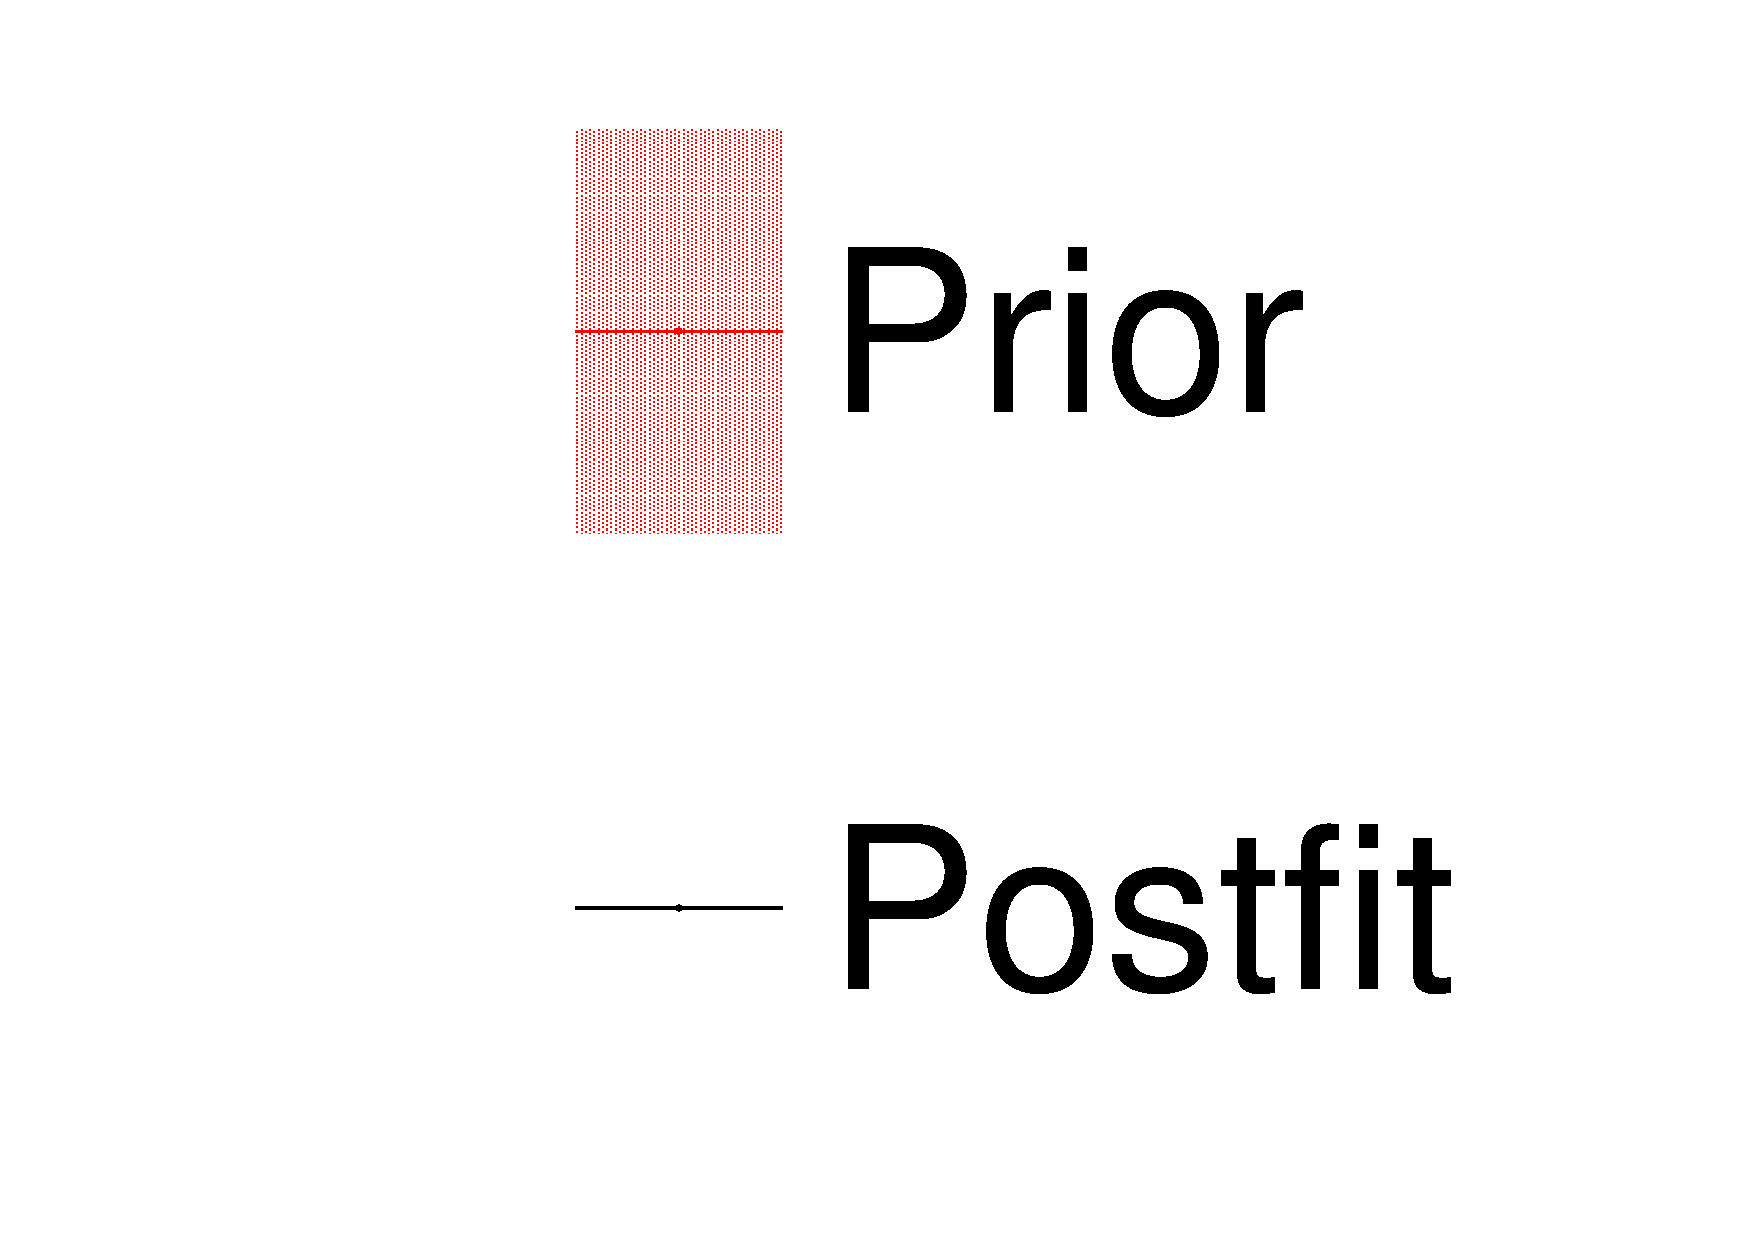
\includegraphics[width=0.24\linewidth]{figs/asmv_leg}
\end{subfigure}
\begin{subfigure}{0.45\textwidth}
  \centering
  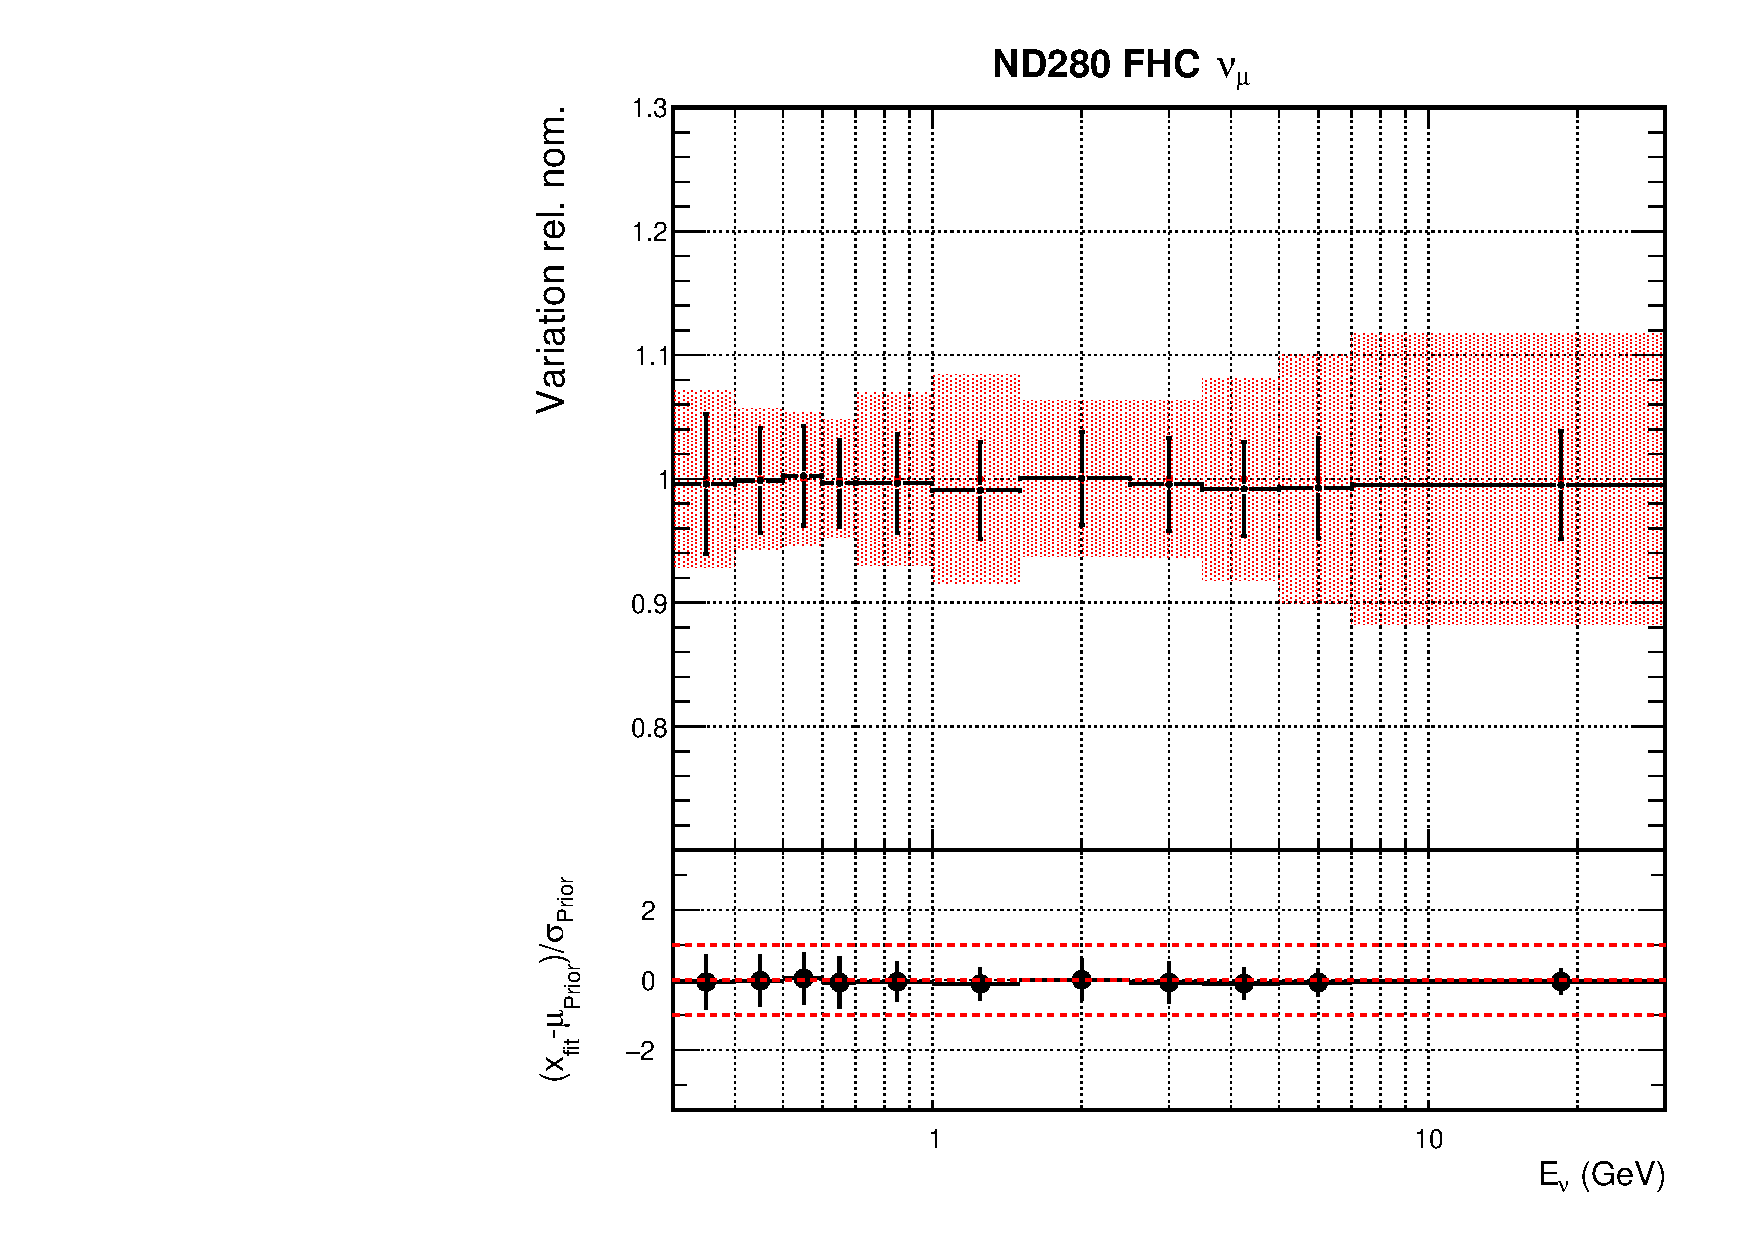
\includegraphics[width=0.75\linewidth]{figs/asmvfluxpoly0}
  \caption{ND FHC $\nu_{\mu}$}
\end{subfigure}
\begin{subfigure}{0.45\textwidth}
  \centering
  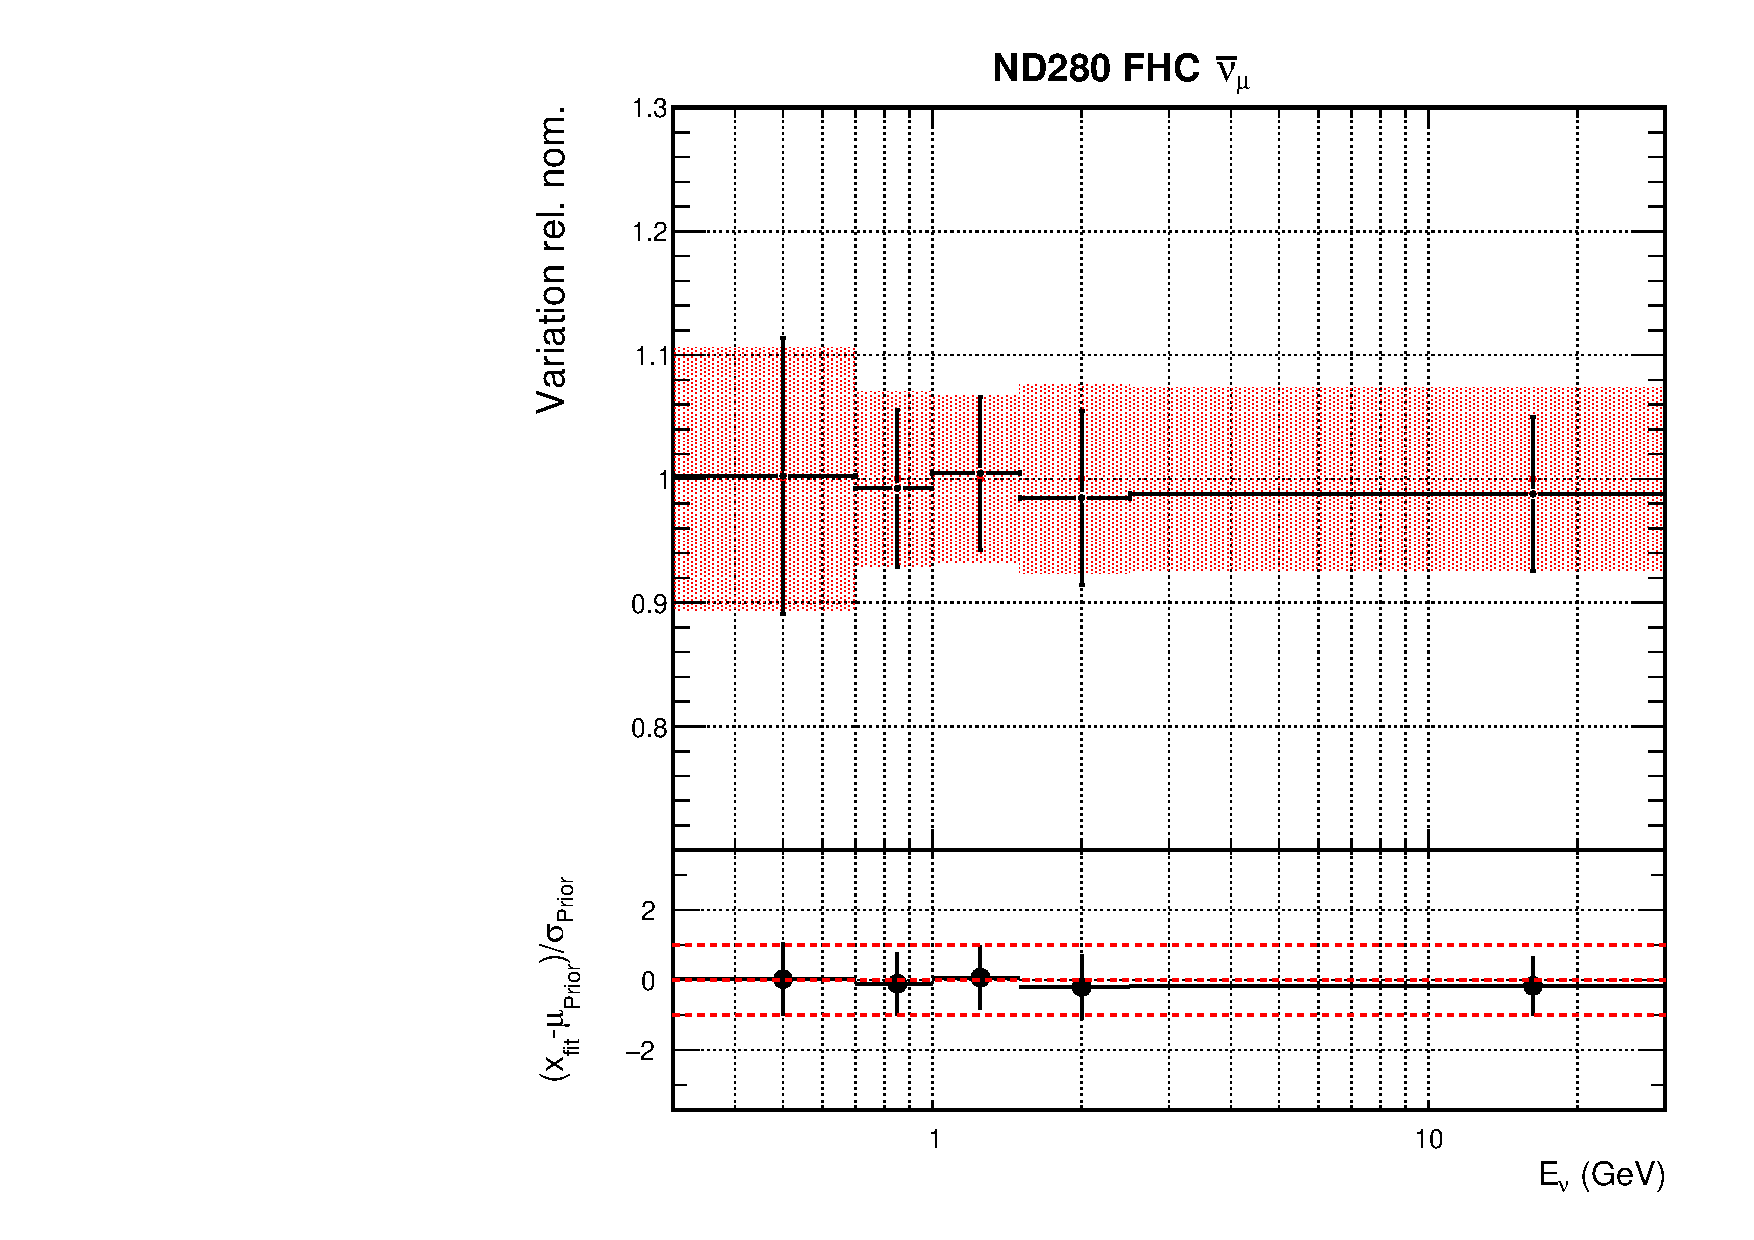
\includegraphics[width=0.75\linewidth]{figs/asmvfluxpoly1}
  \caption{ND FHC $\bar{\nu_{\mu}}$}
\end{subfigure}
\begin{subfigure}{0.45\textwidth}
  \centering
  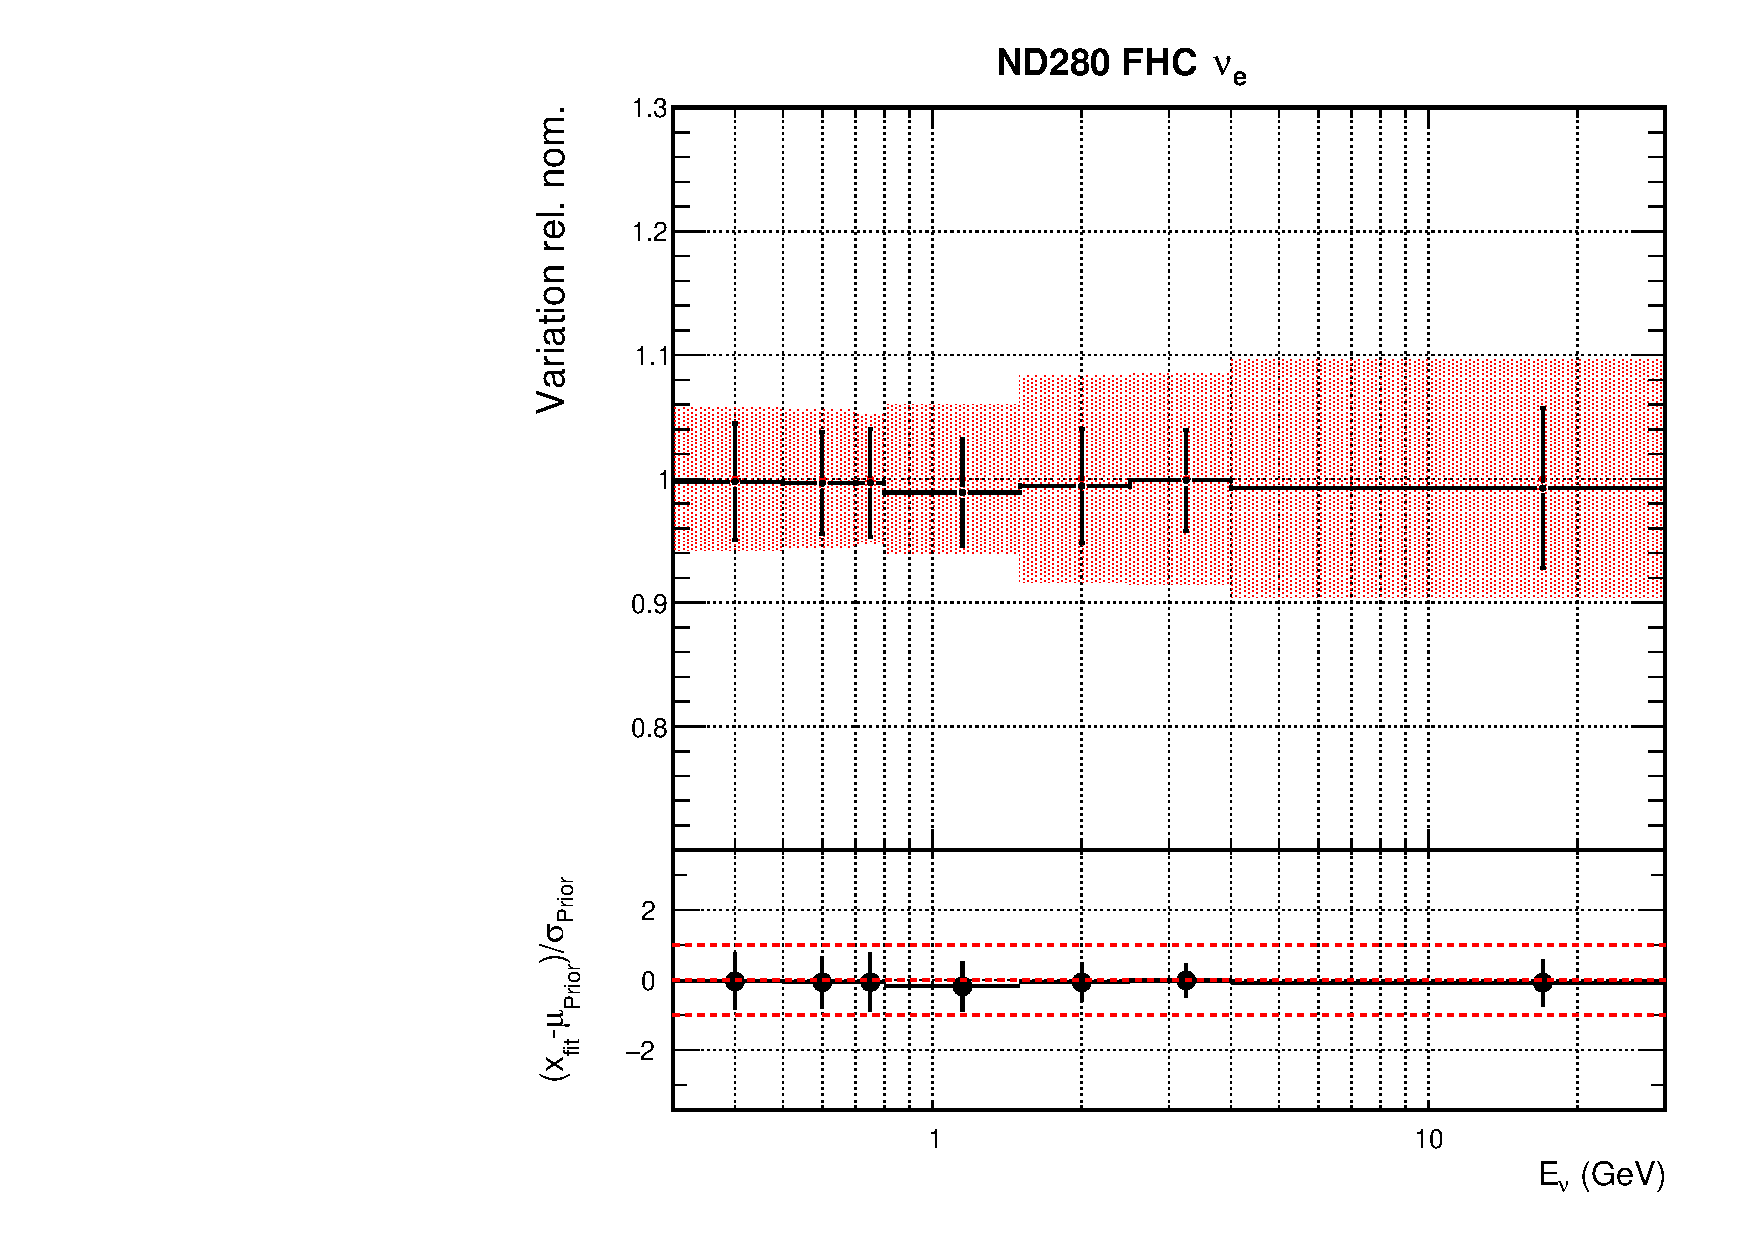
\includegraphics[width=0.75\linewidth]{figs/asmvfluxpoly2}
  \caption{ND FHC $\nu_e$}
\end{subfigure}
\begin{subfigure}{0.45\textwidth}
  \centering
  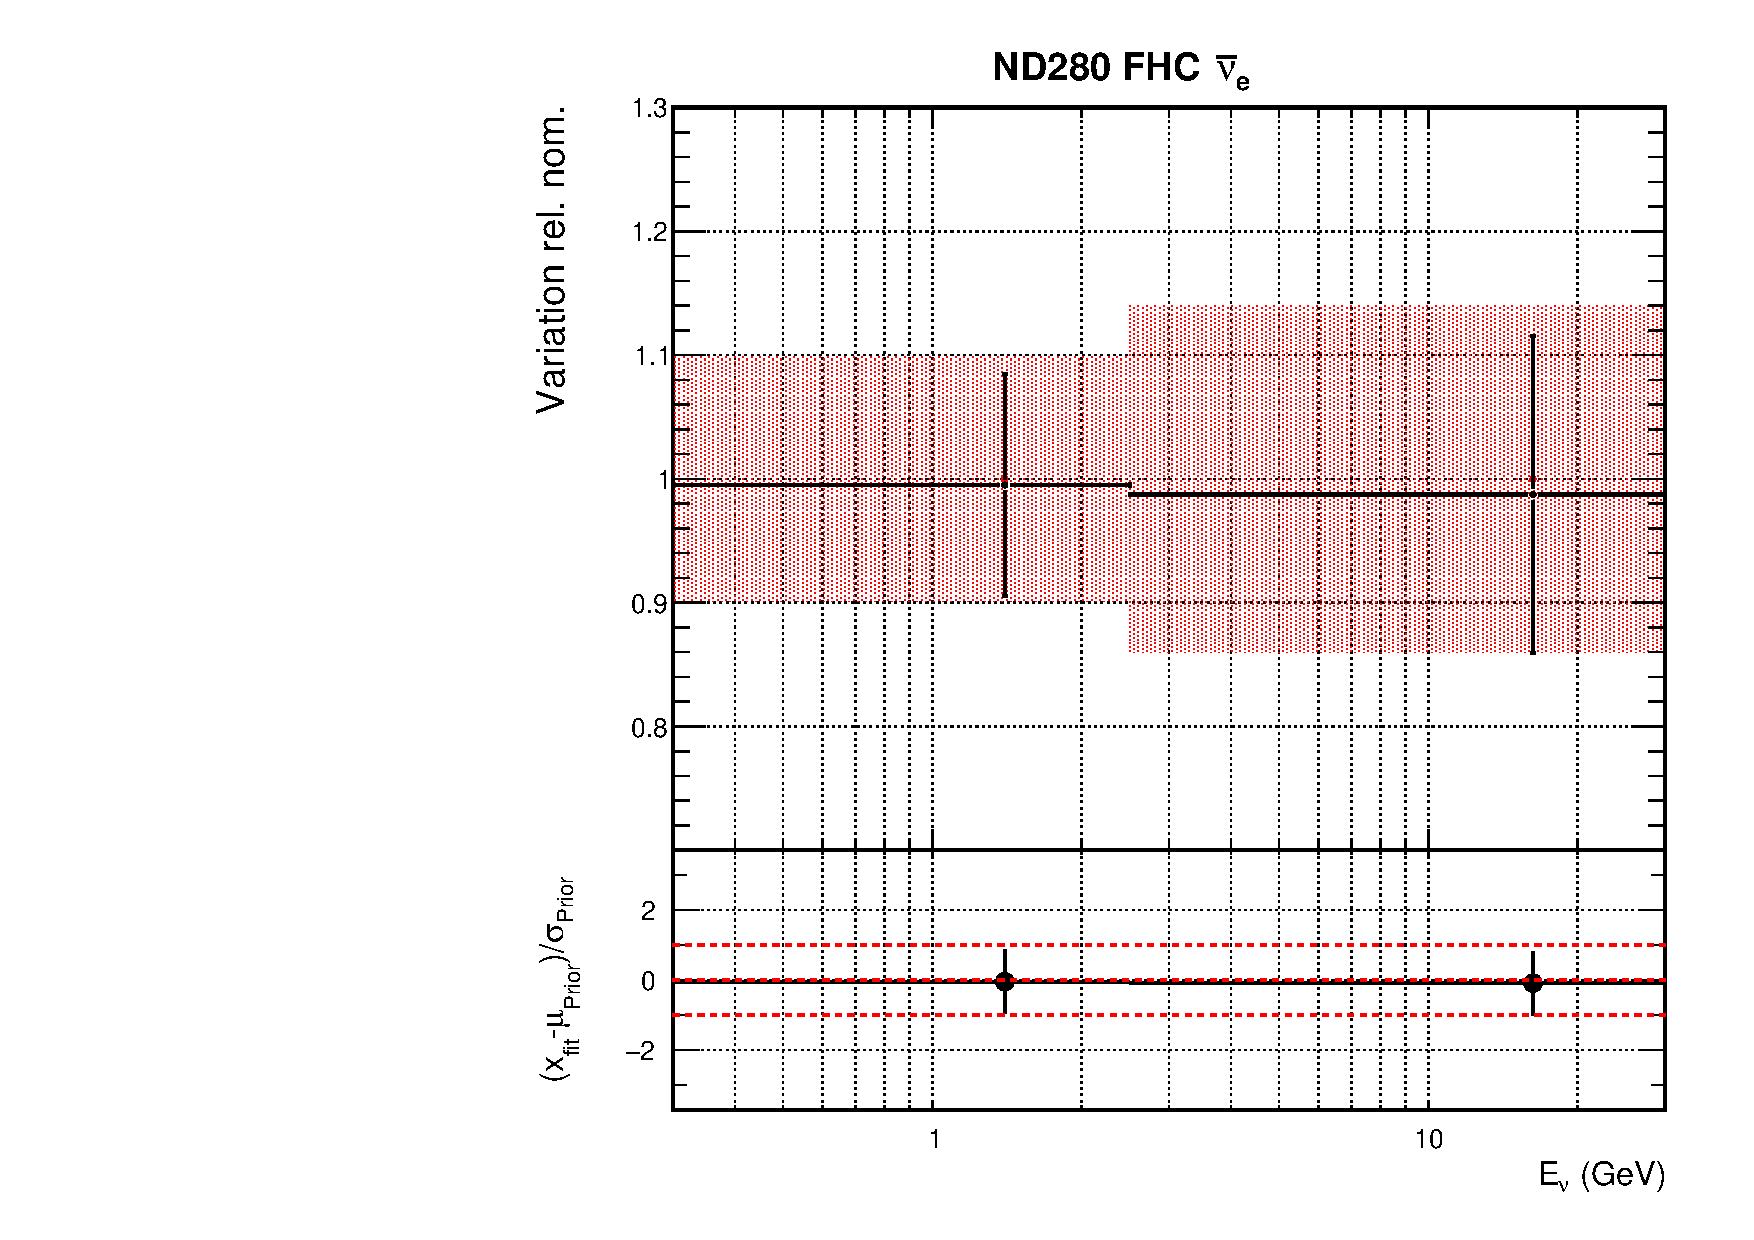
\includegraphics[width=0.75\linewidth]{figs/asmvfluxpoly3}
  \caption{ND FHC $\bar{\nu_{e}}$}
\end{subfigure}
\begin{subfigure}{0.45\textwidth}
  \centering
  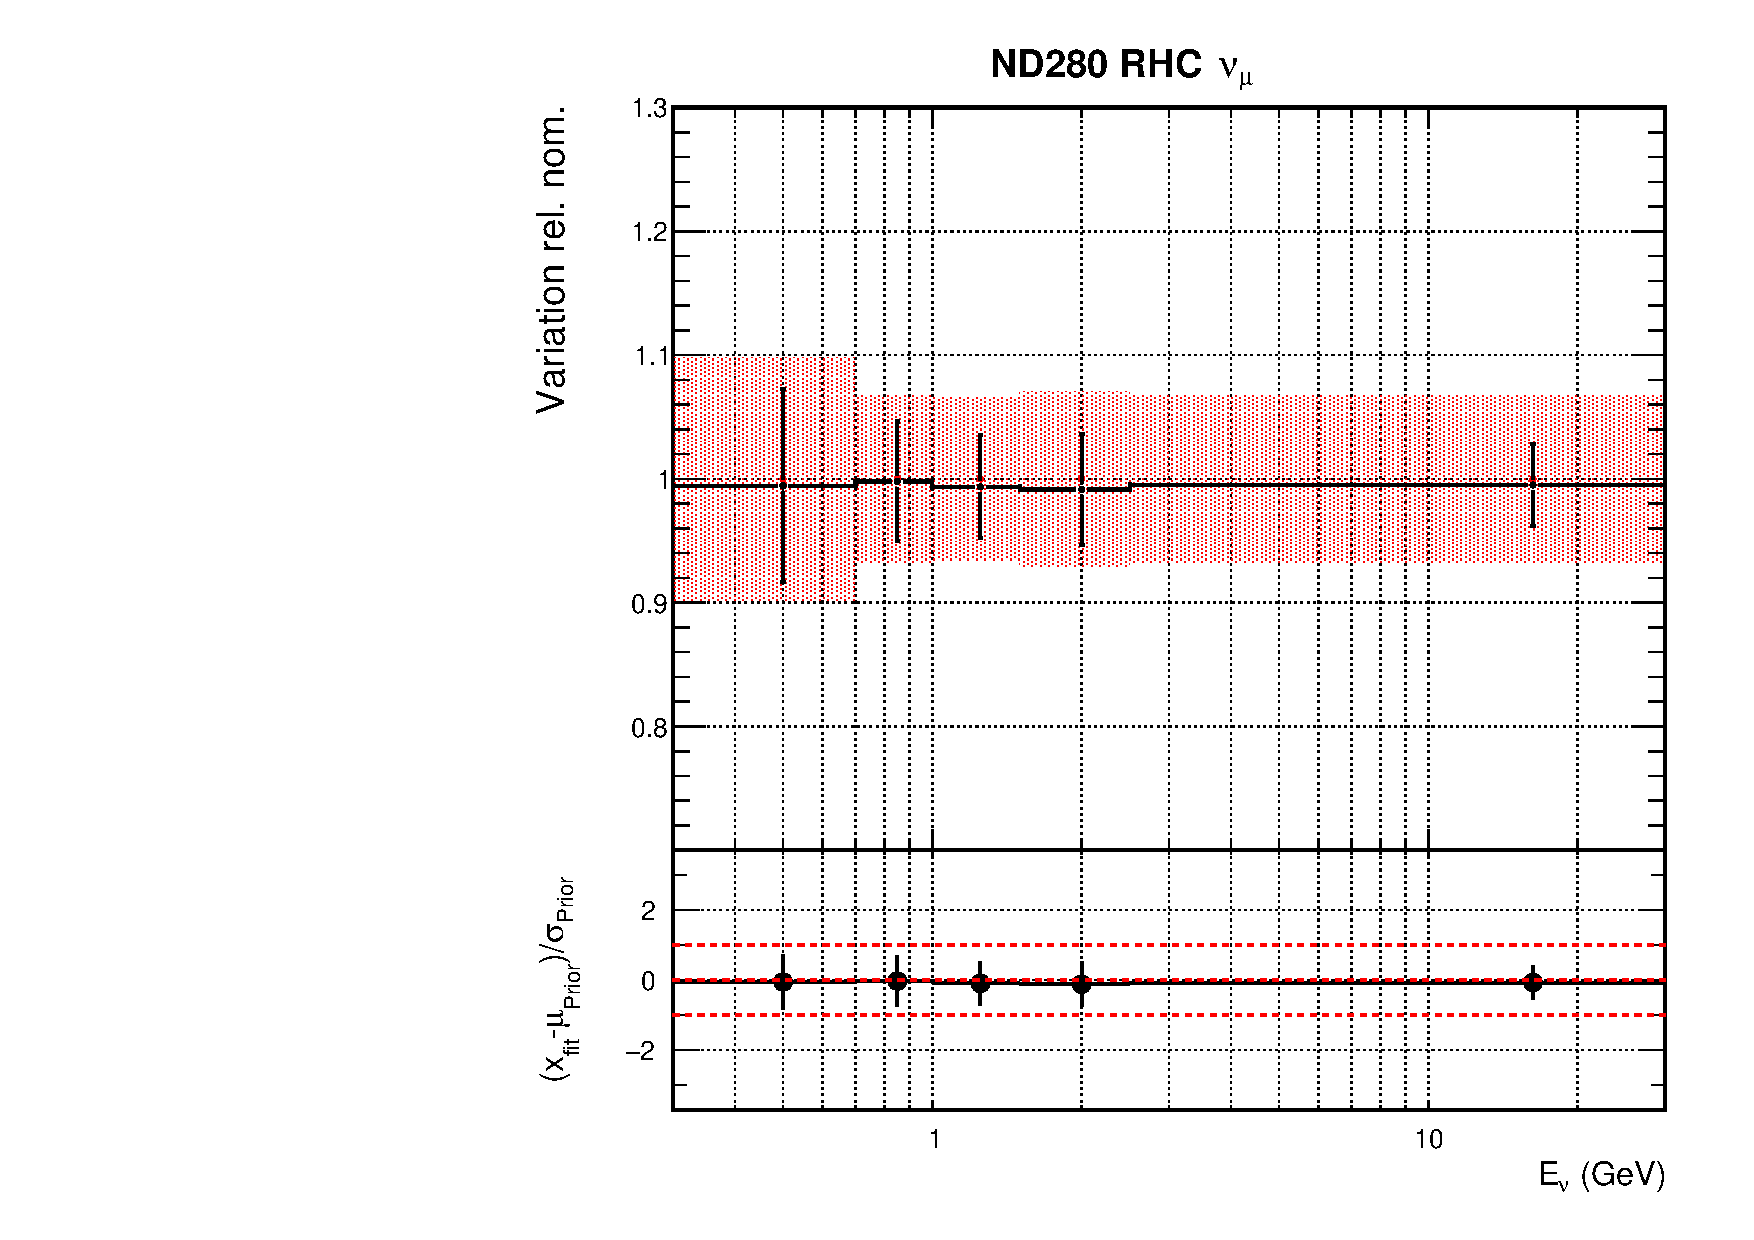
\includegraphics[width=0.75\linewidth]{figs/asmvfluxpoly4}
  \caption{ND RHC $\nu_{\mu}$}
\end{subfigure}
\begin{subfigure}{0.45\textwidth}
  \centering
  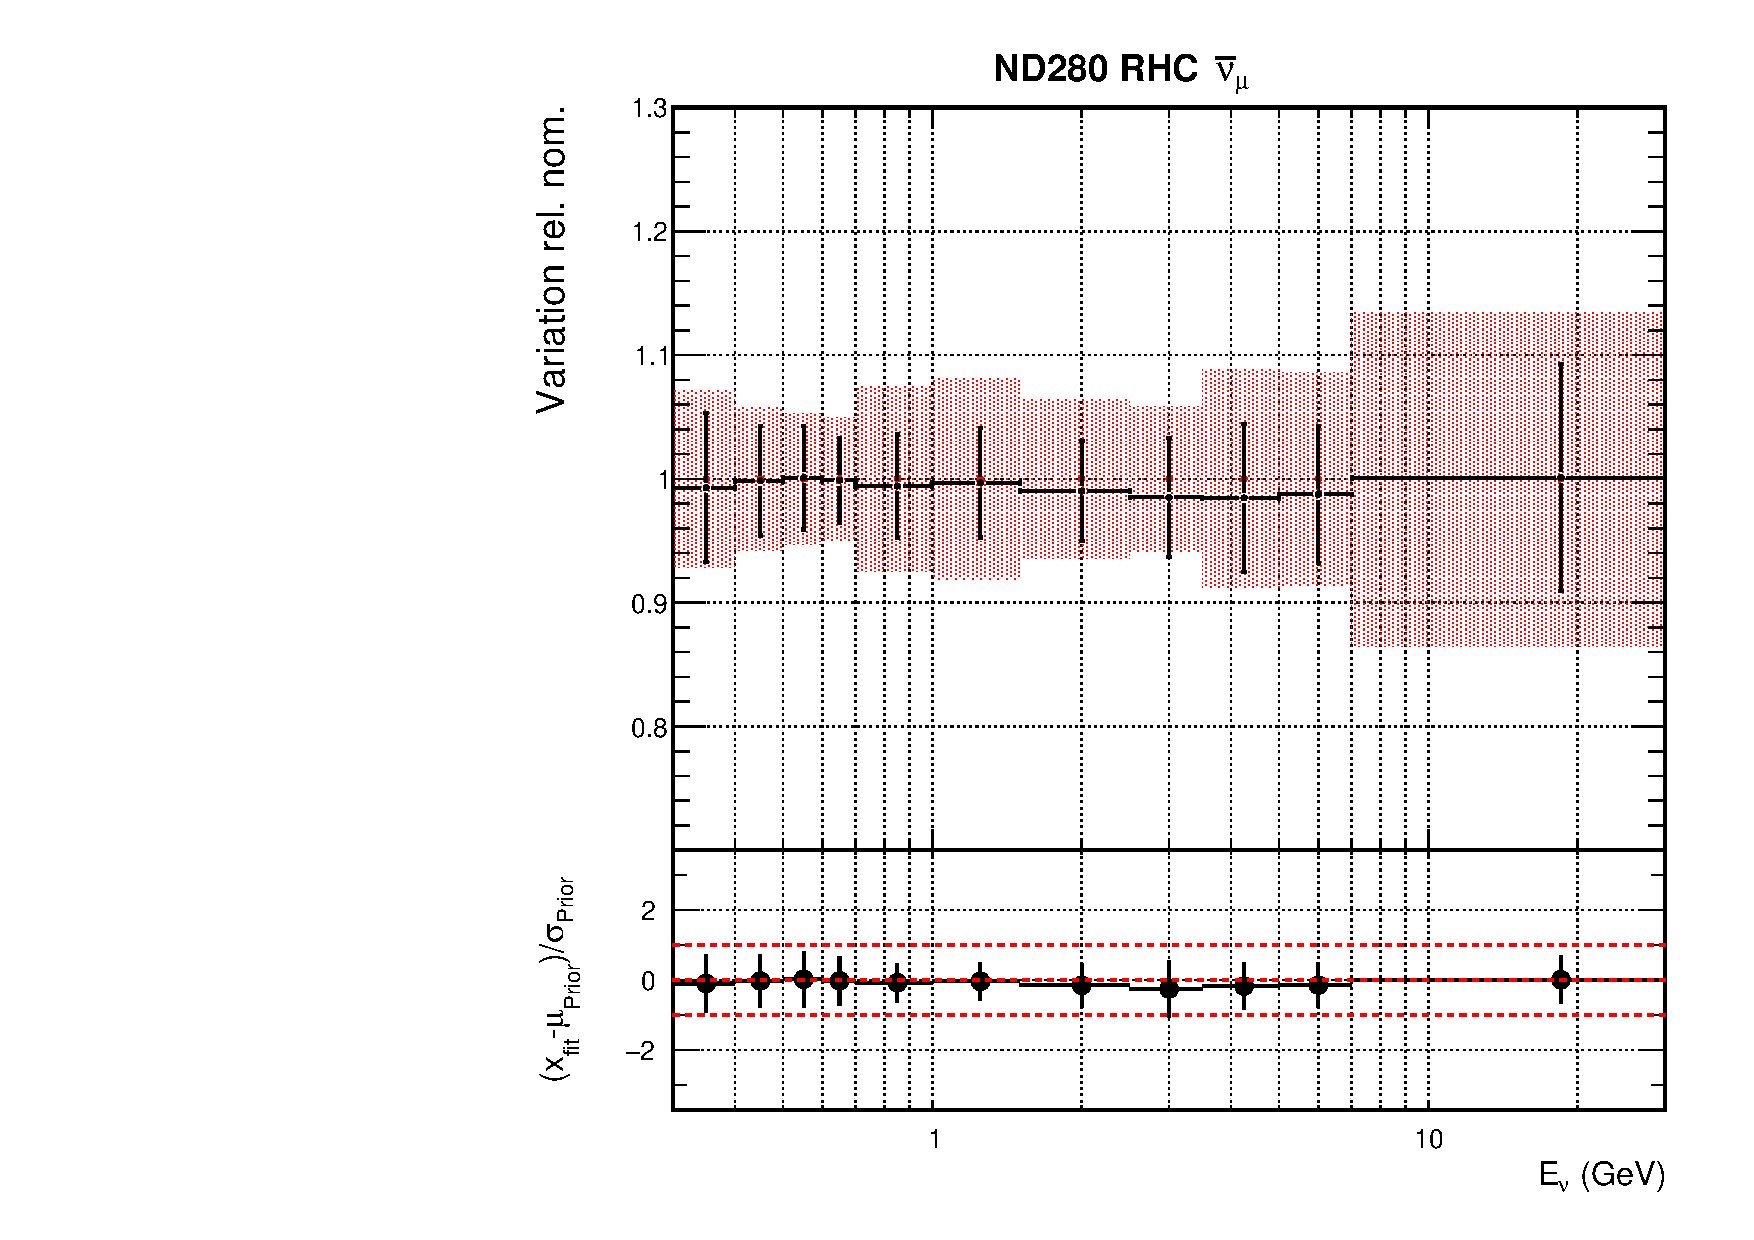
\includegraphics[width=0.75\linewidth]{figs/asmvfluxpoly5}
  \caption{ND RHC $\bar{\nu_{\mu}}$}
\end{subfigure}
\begin{subfigure}{0.45\textwidth}
  \centering
  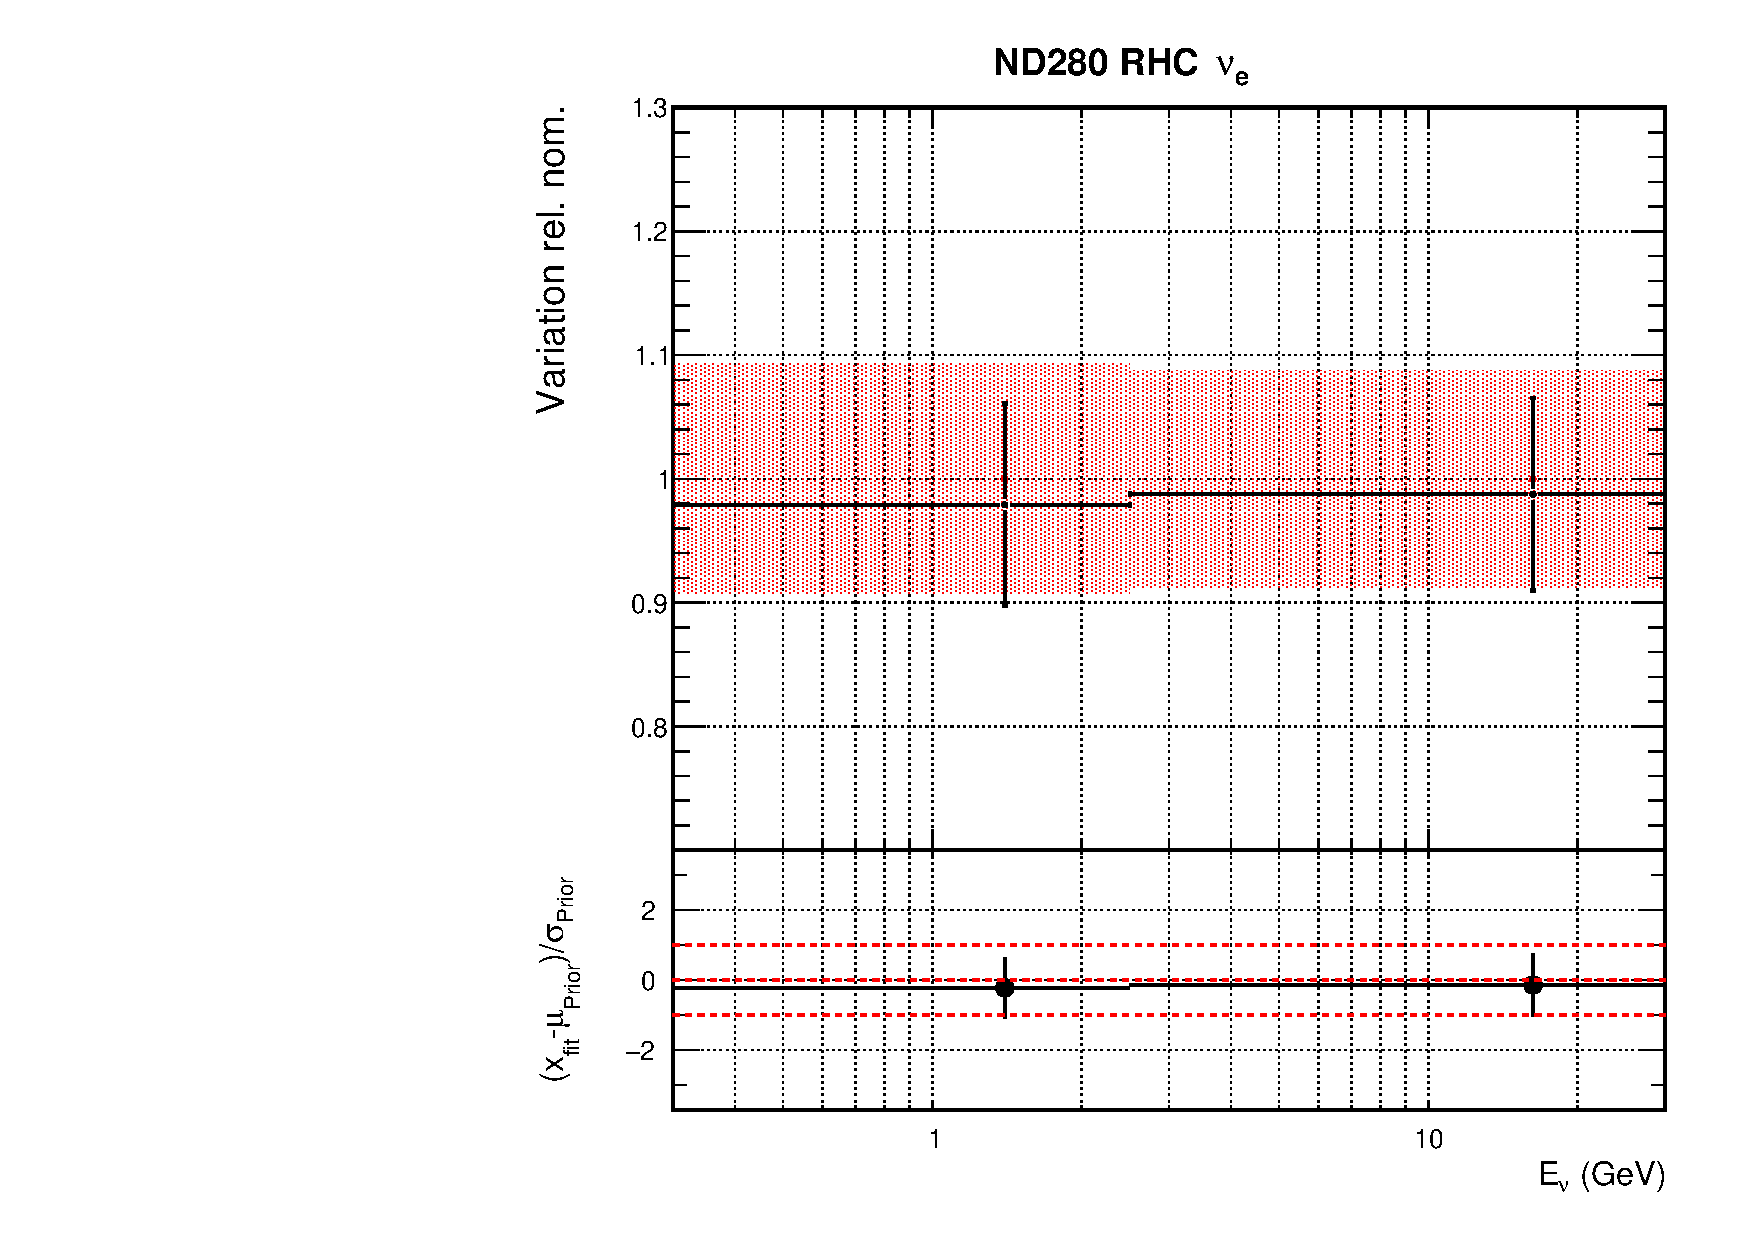
\includegraphics[width=0.75\linewidth]{figs/asmvfluxpoly6}
  \caption{ND RHC $\nu_{e}$}
\end{subfigure}
\begin{subfigure}{0.45\textwidth}
  \centering
  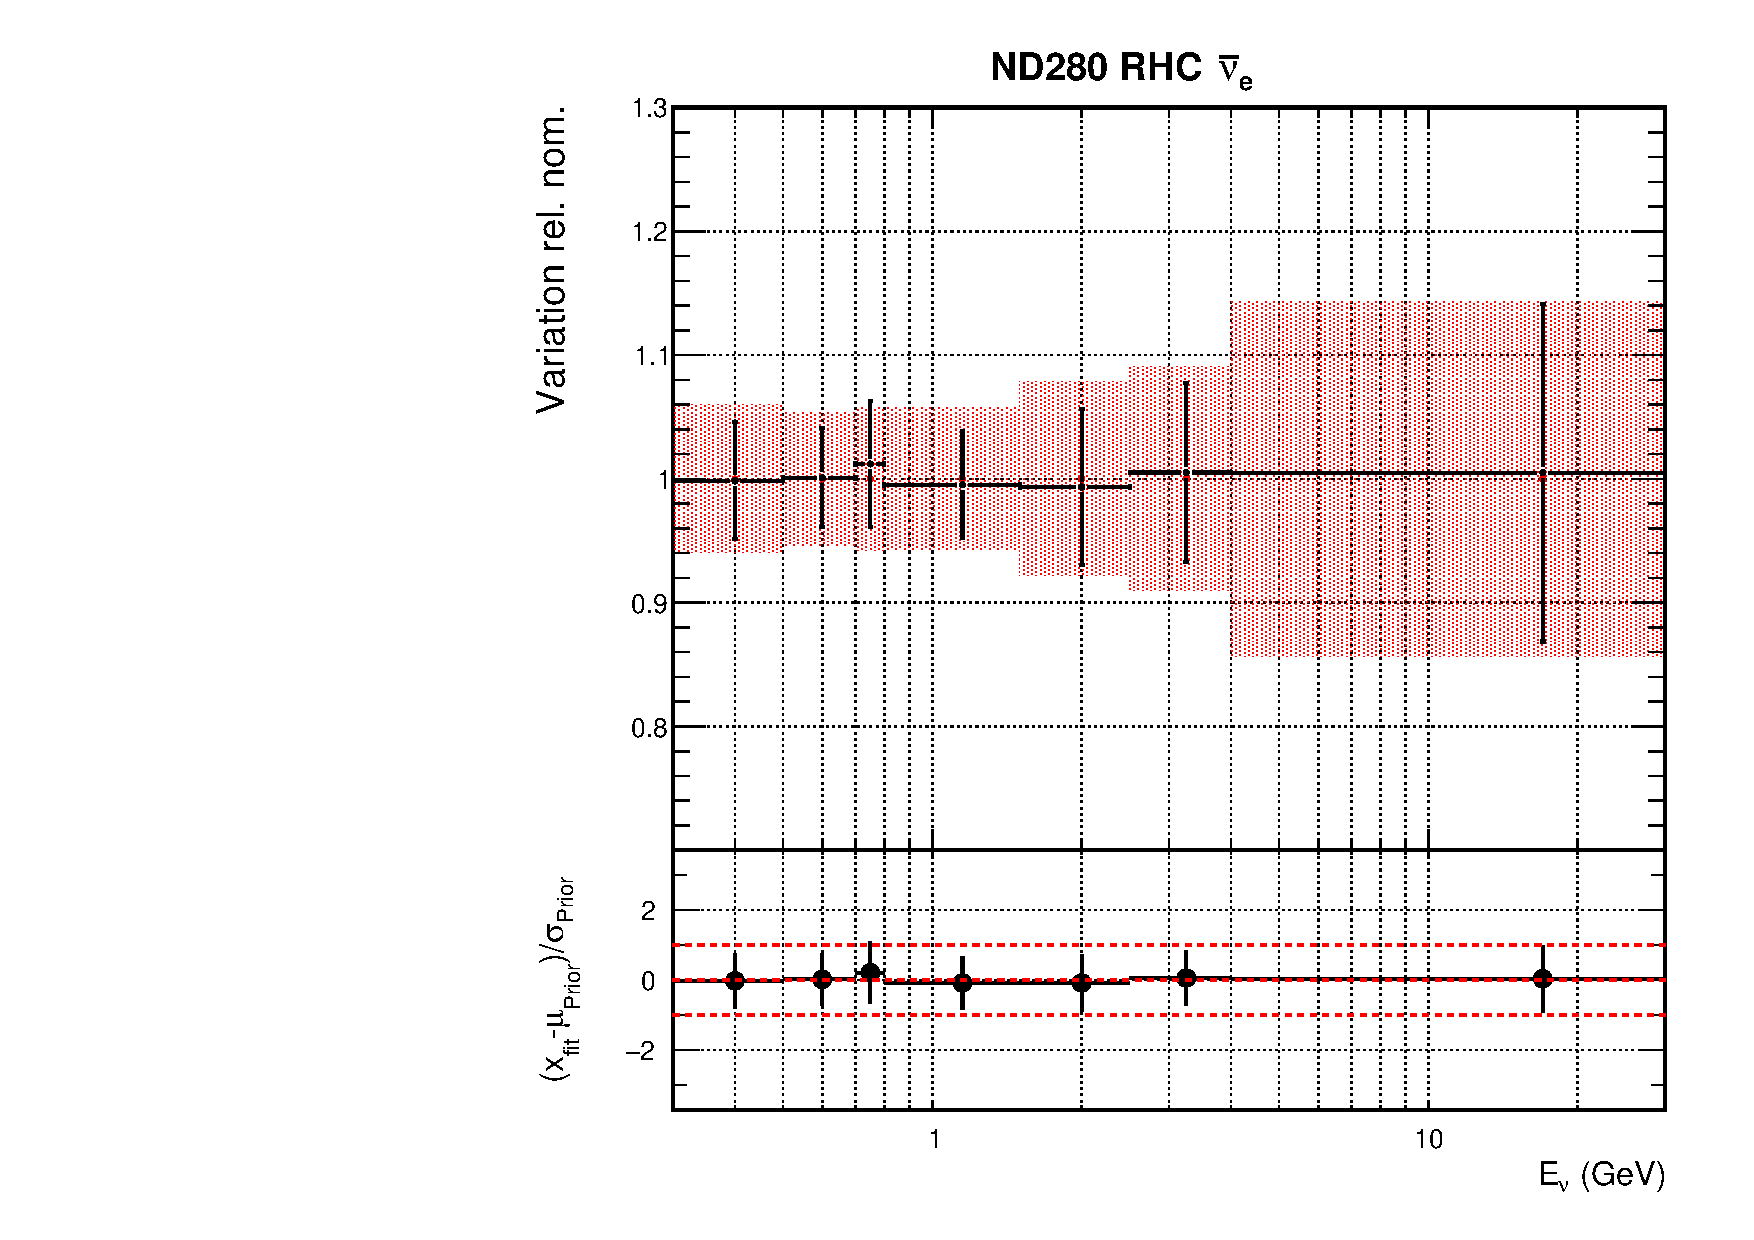
\includegraphics[width=0.75\linewidth]{figs/asmvfluxpoly7}
  \caption{ND RHC $\bar{\nu_e}$}
\end{subfigure}
\caption{ND280 flux parameters for the Asimov fit.}
\label{fig:asmvfluxNDapp}
\end{figure}

\begin{figure}[!htbp]
\centering
\begin{subfigure}{0.8\textwidth}
  \centering
  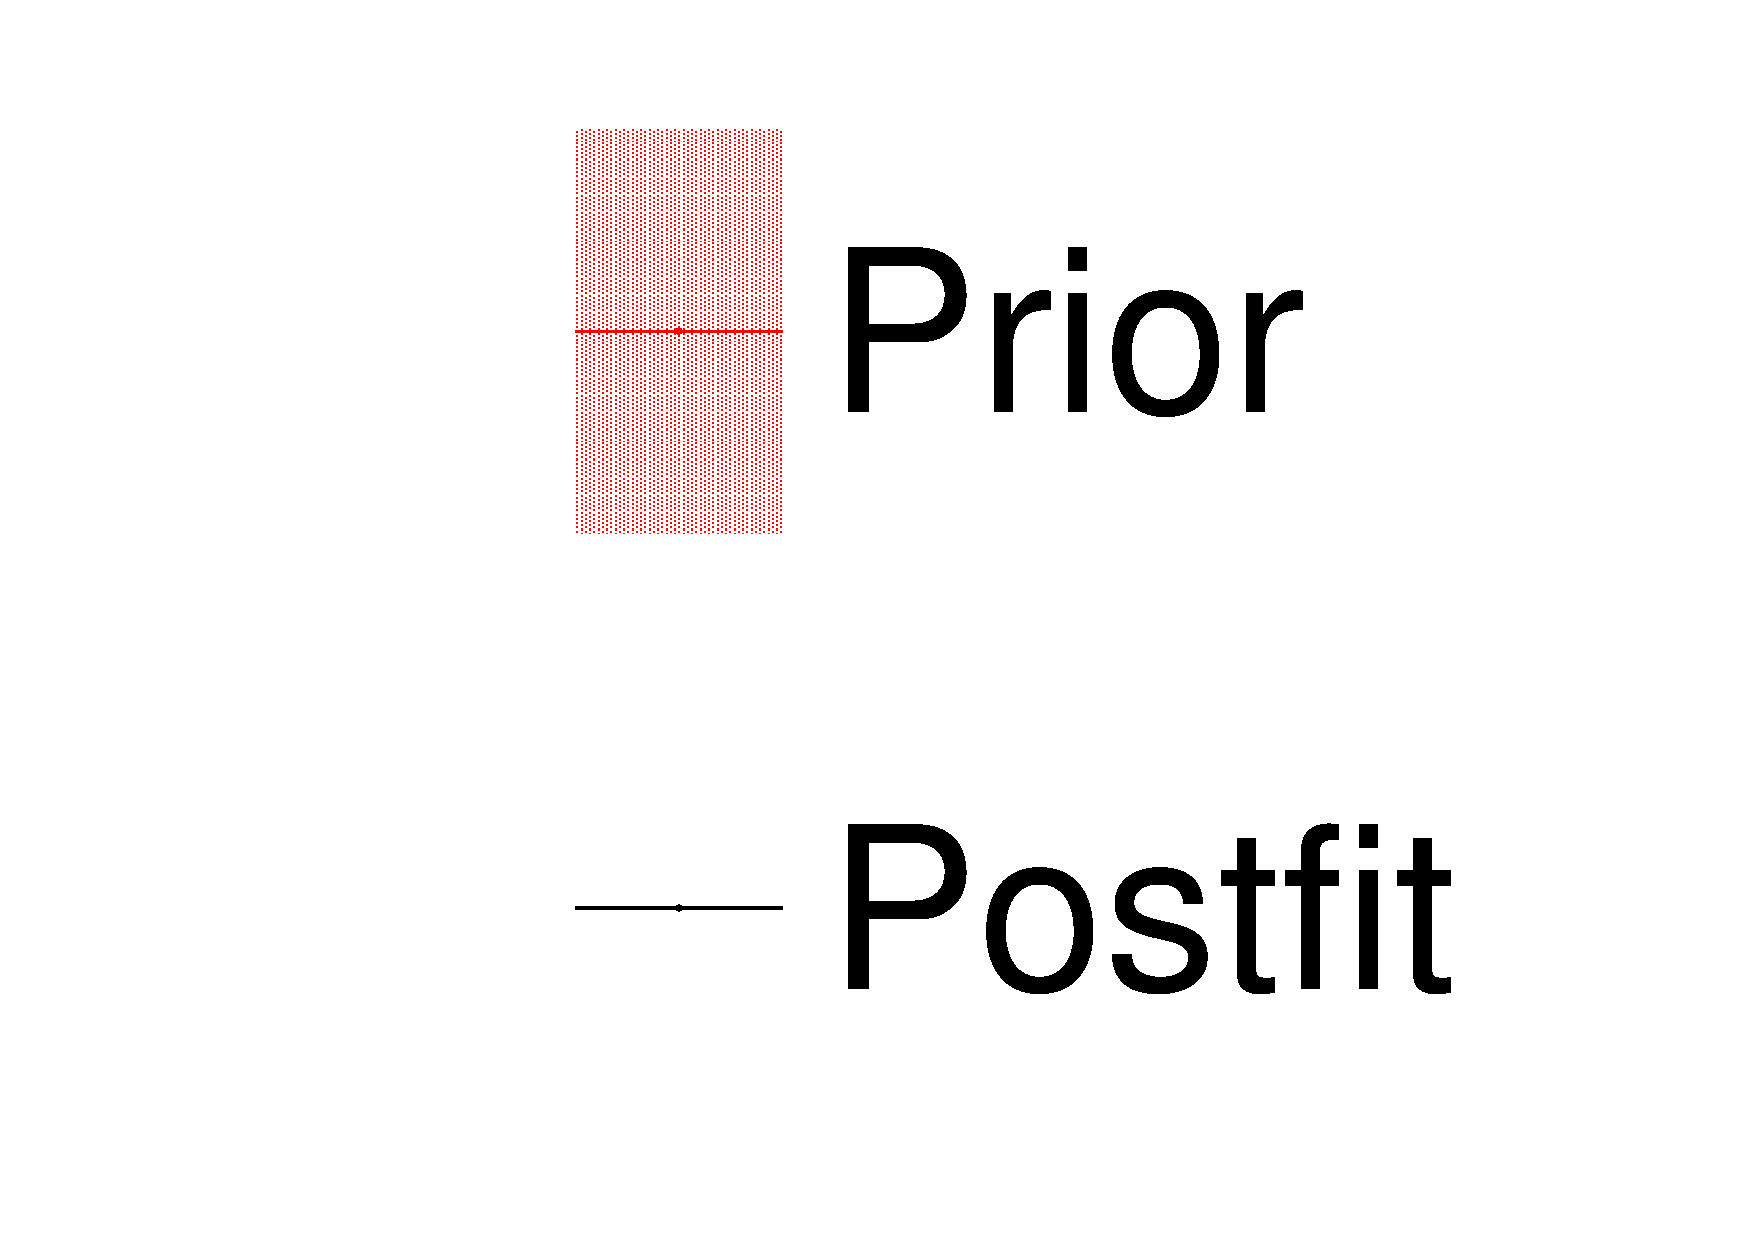
\includegraphics[width=0.24\linewidth]{figs/asmv_leg}
\end{subfigure}
\begin{subfigure}{0.45\textwidth}
  \centering
  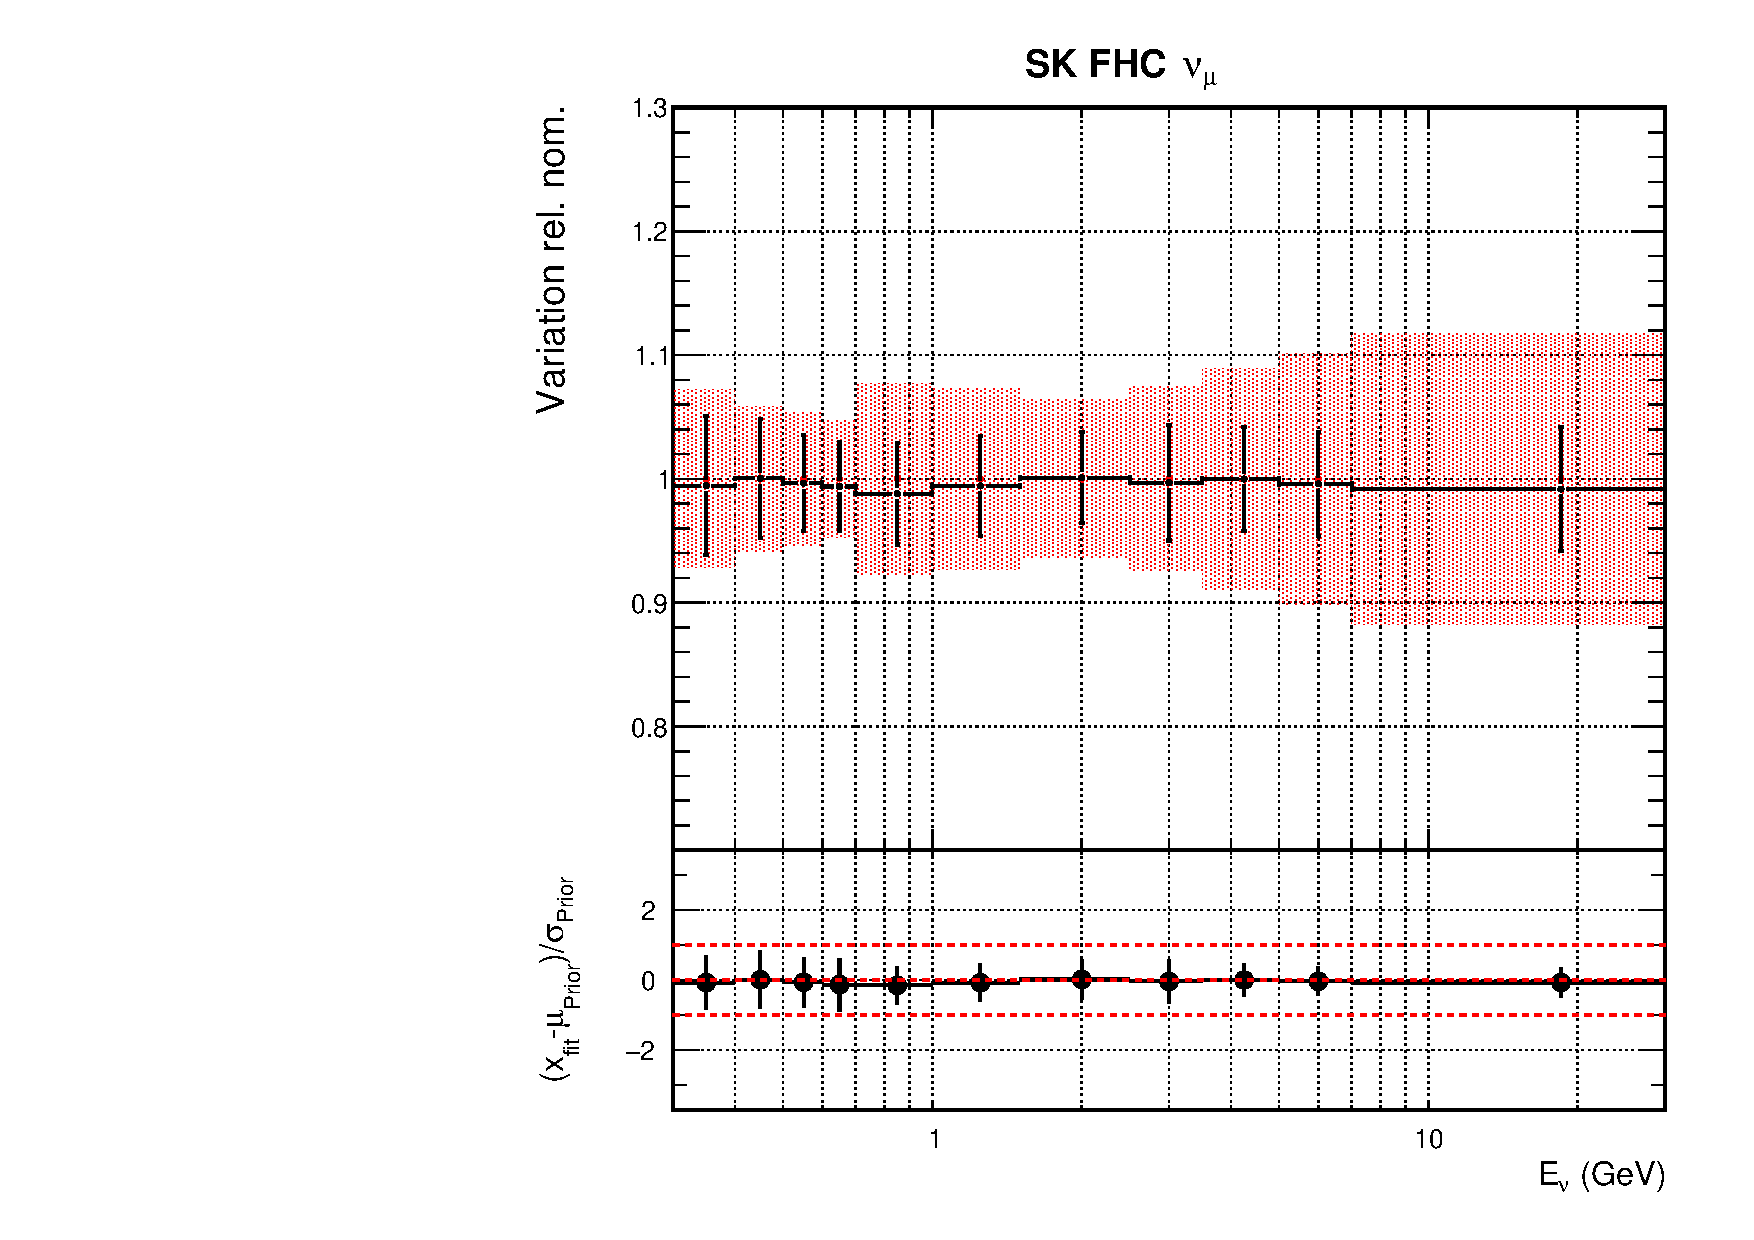
\includegraphics[width=0.75\linewidth]{figs/asmvfluxpoly8}
  \caption{\SK FHC $\nu_{\mu}$}
\end{subfigure}
\begin{subfigure}{0.45\textwidth}
  \centering
  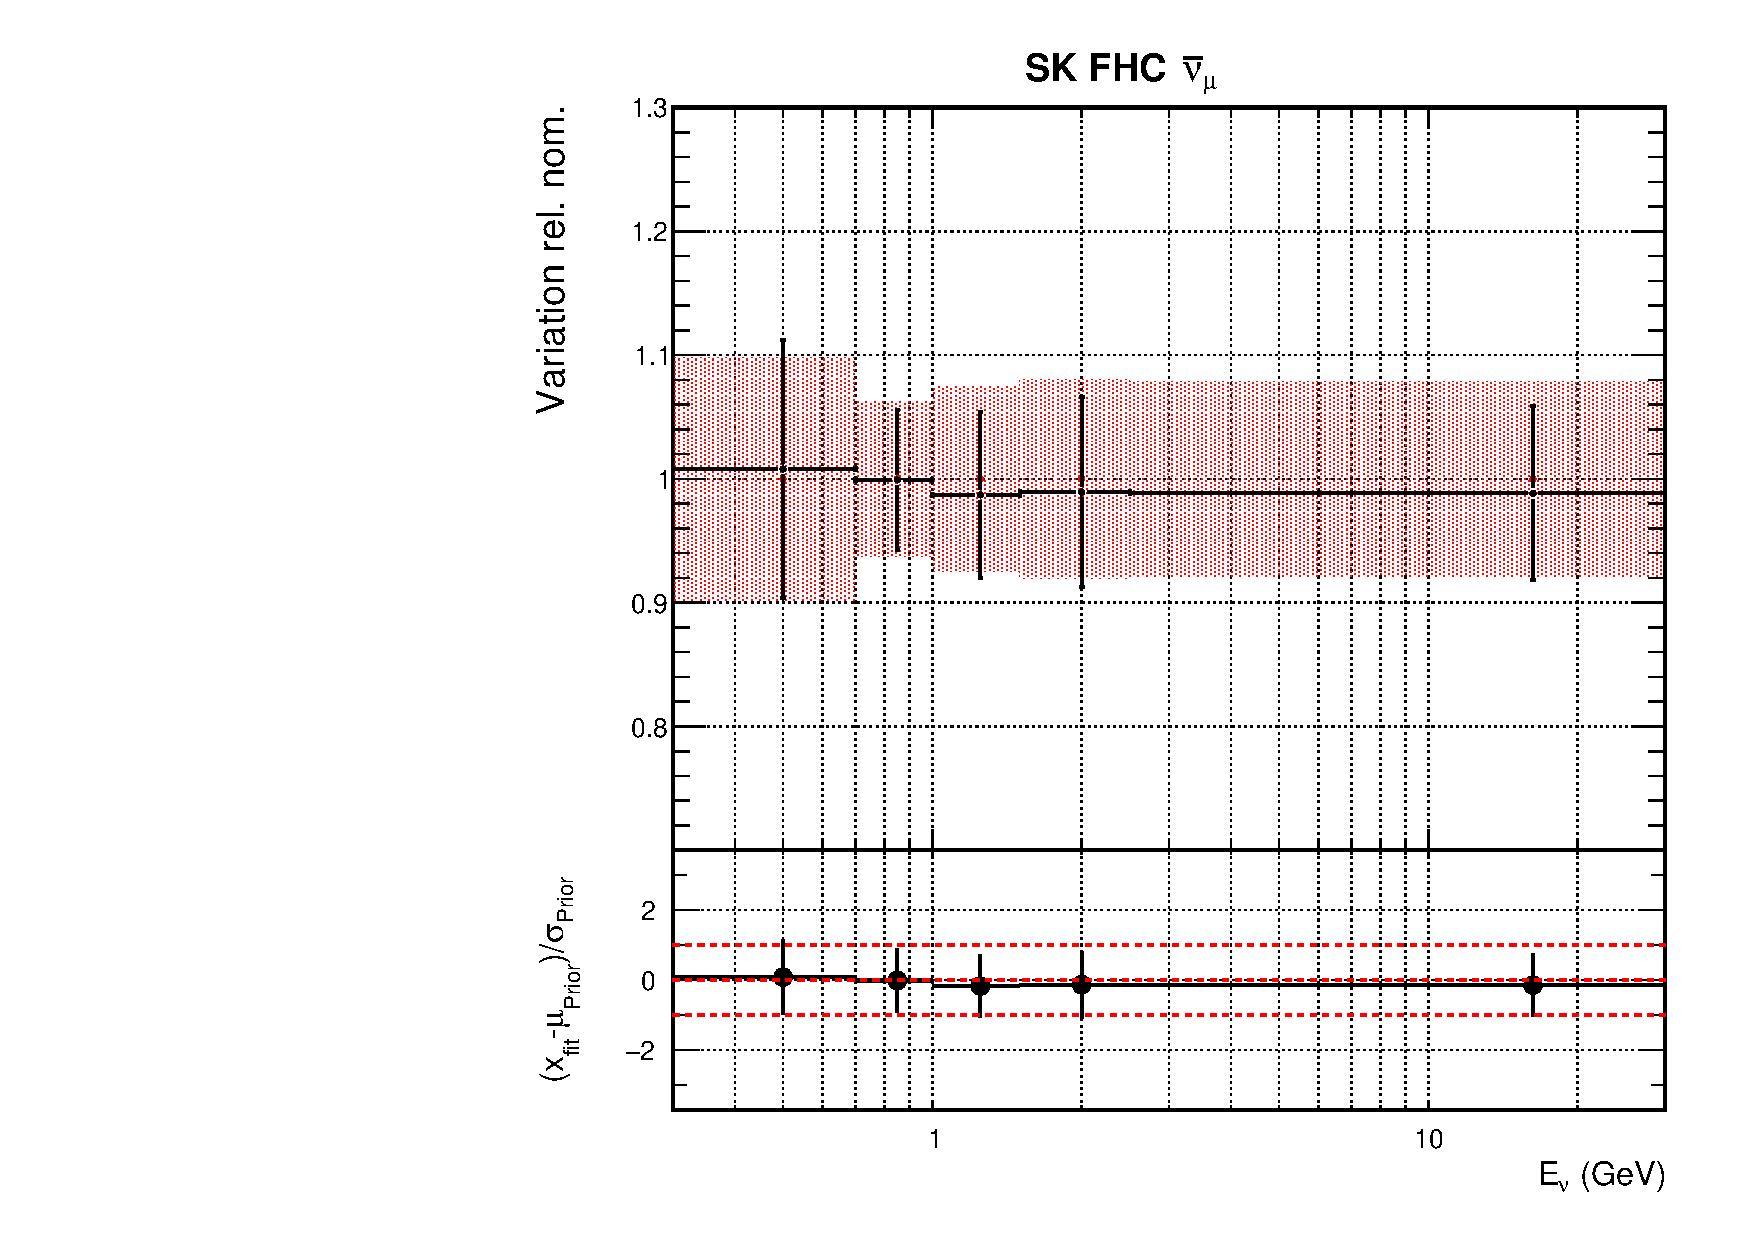
\includegraphics[width=0.75\linewidth]{figs/asmvfluxpoly9}
  \caption{\SK FHC $\bar{\nu_{\mu}}$}
\end{subfigure}
\begin{subfigure}{0.45\textwidth}
  \centering
  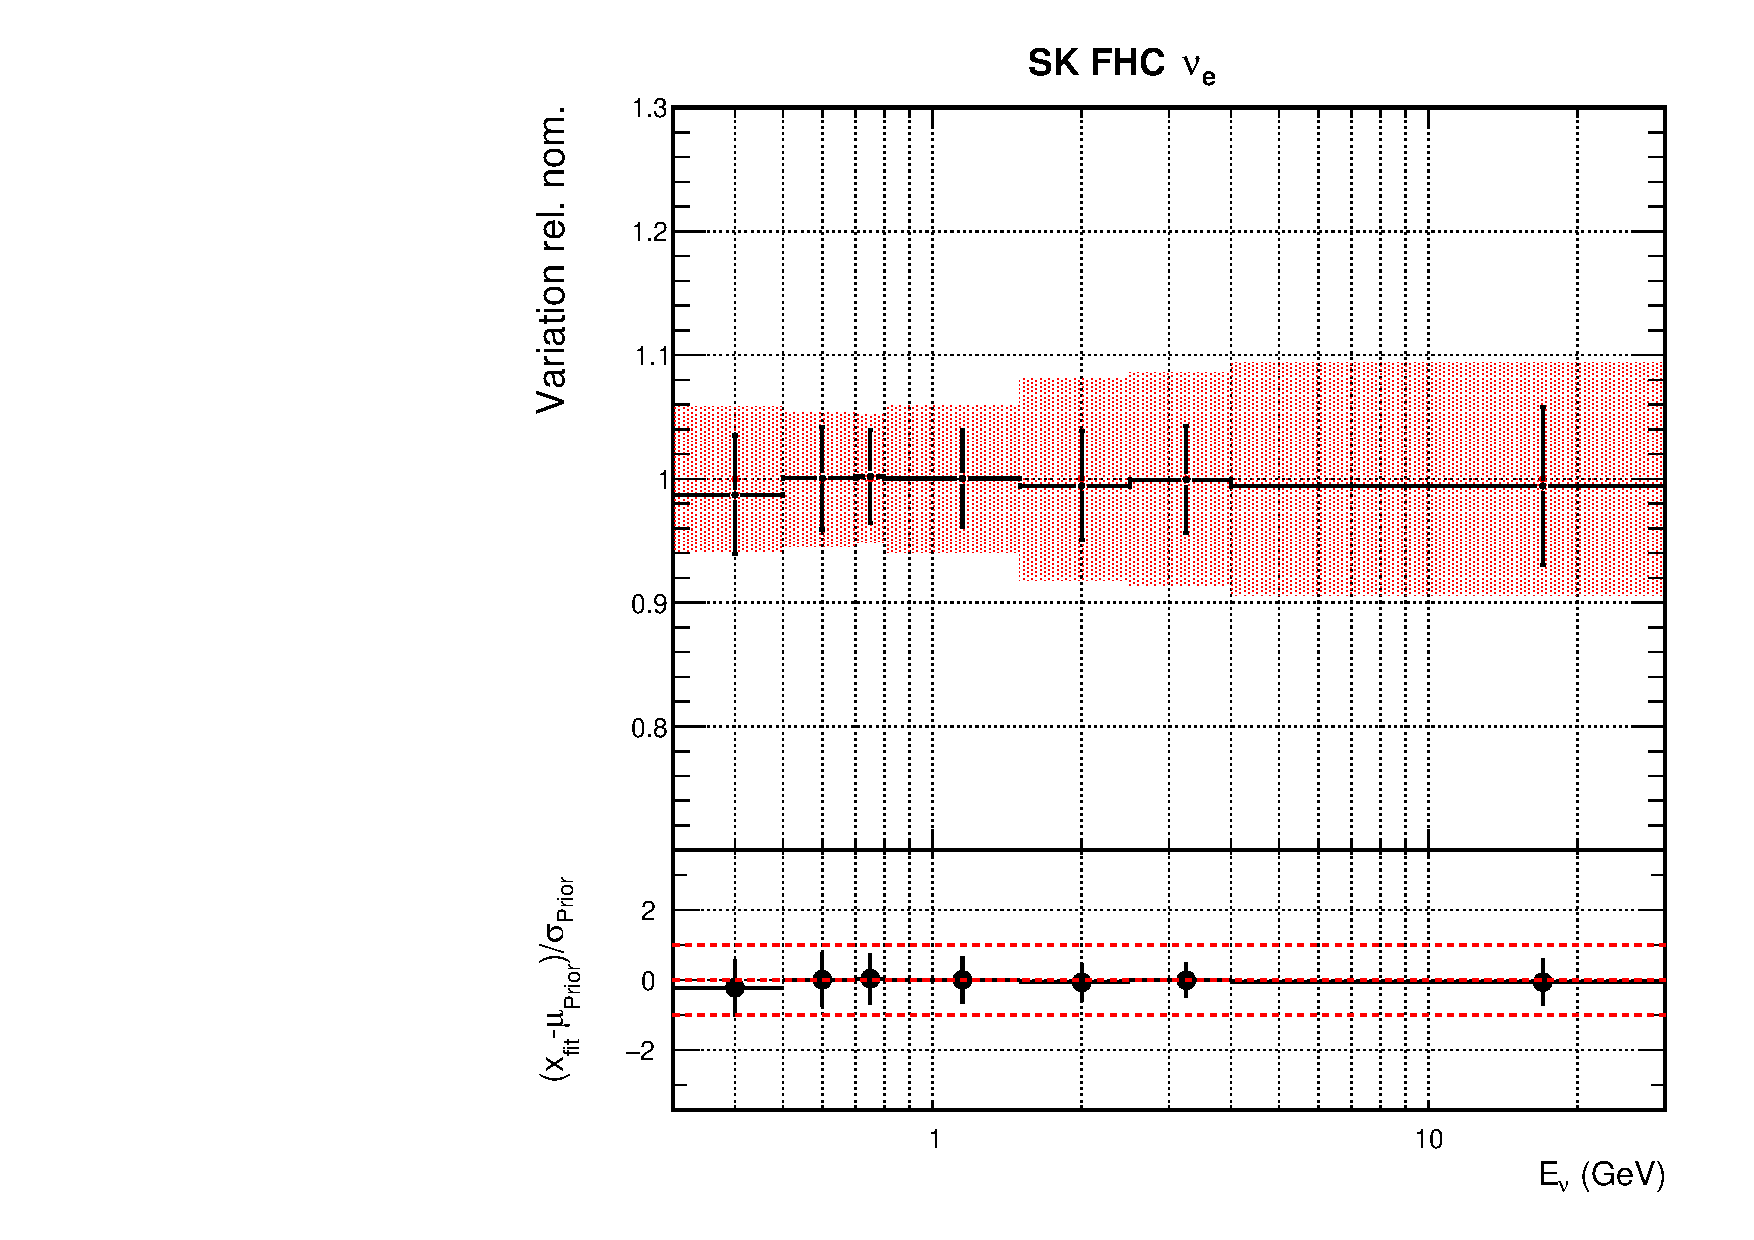
\includegraphics[width=0.75\linewidth]{figs/asmvfluxpoly10}
  \caption{\SK FHC $\nu_{e}$}
\end{subfigure}
\begin{subfigure}{0.45\textwidth}
  \centering
  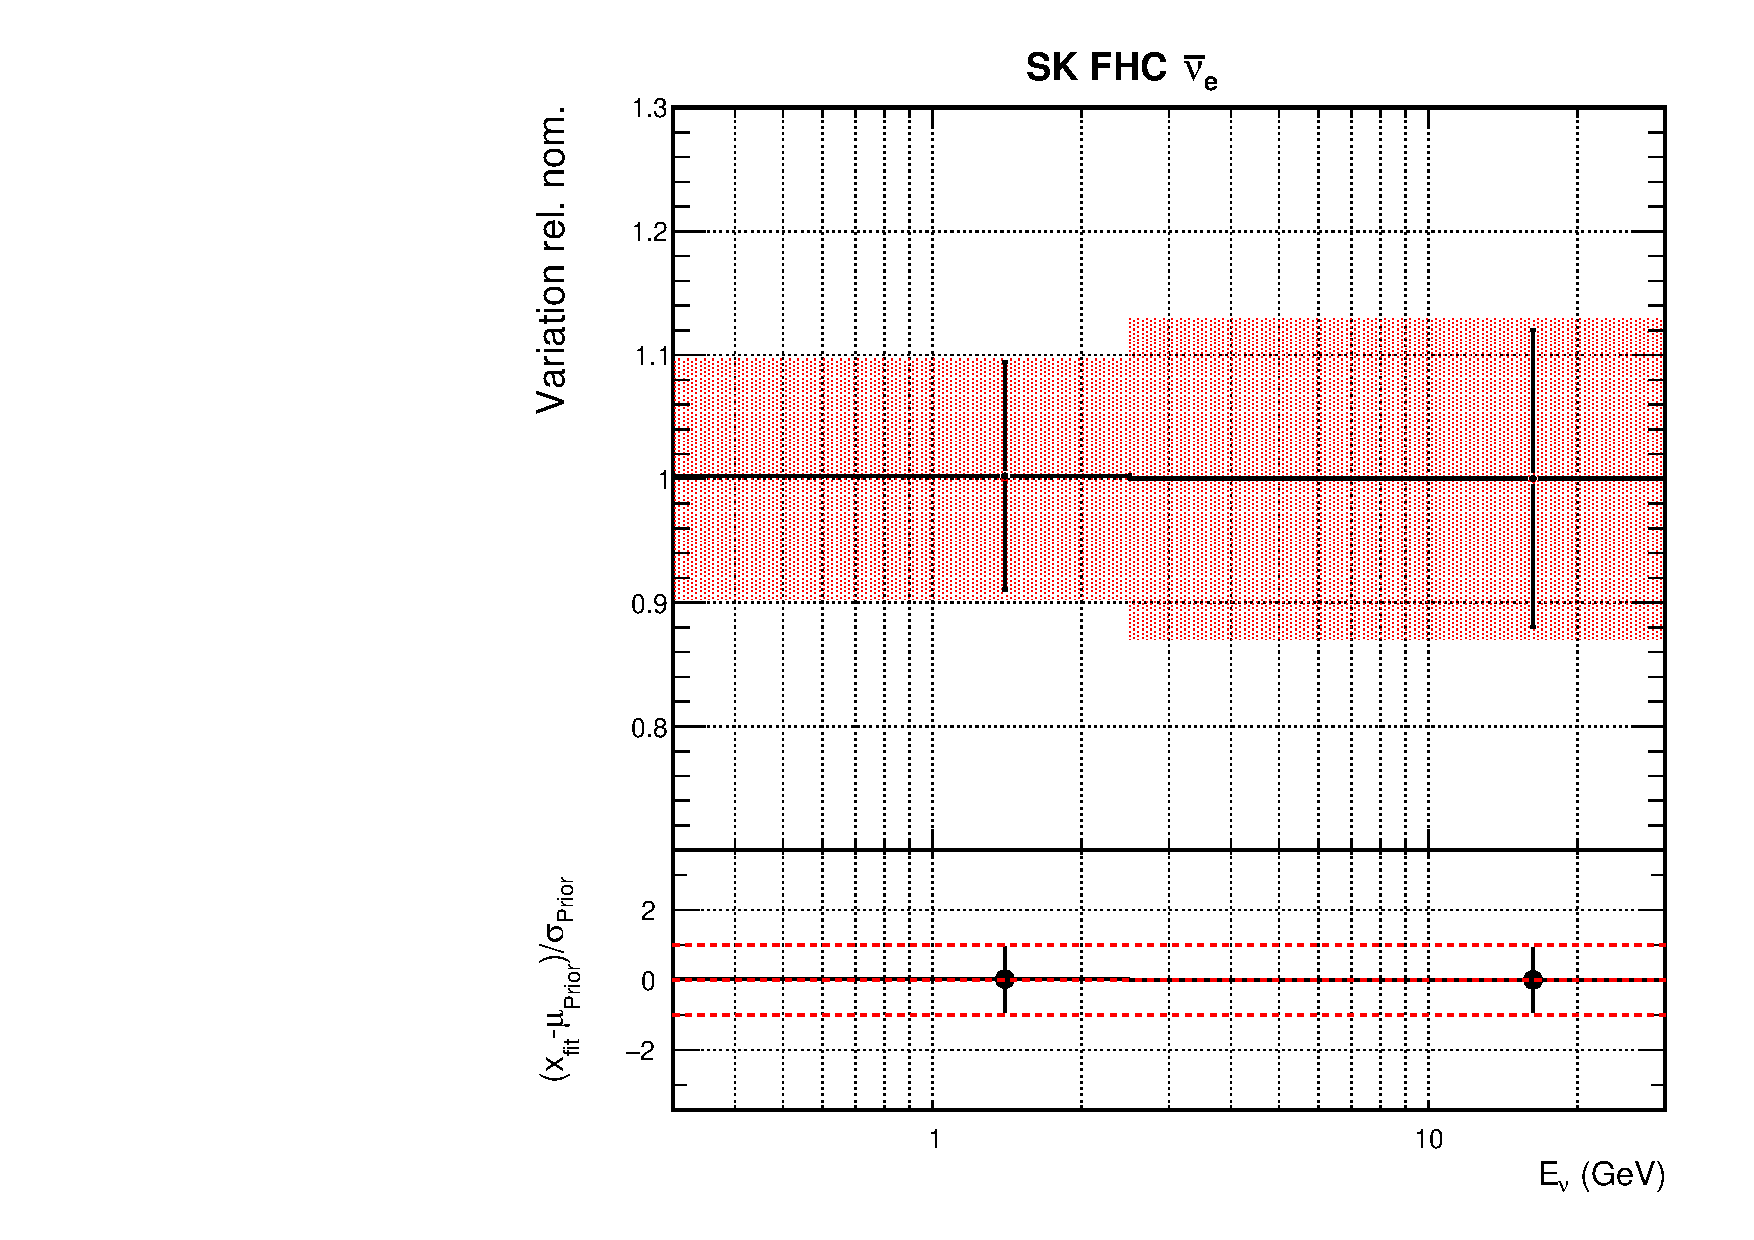
\includegraphics[width=0.75\linewidth]{figs/asmvfluxpoly11}
  \caption{\SK FHC $\bar{\nu_{e}}$}
\end{subfigure}
\begin{subfigure}{0.45\textwidth}
  \centering
  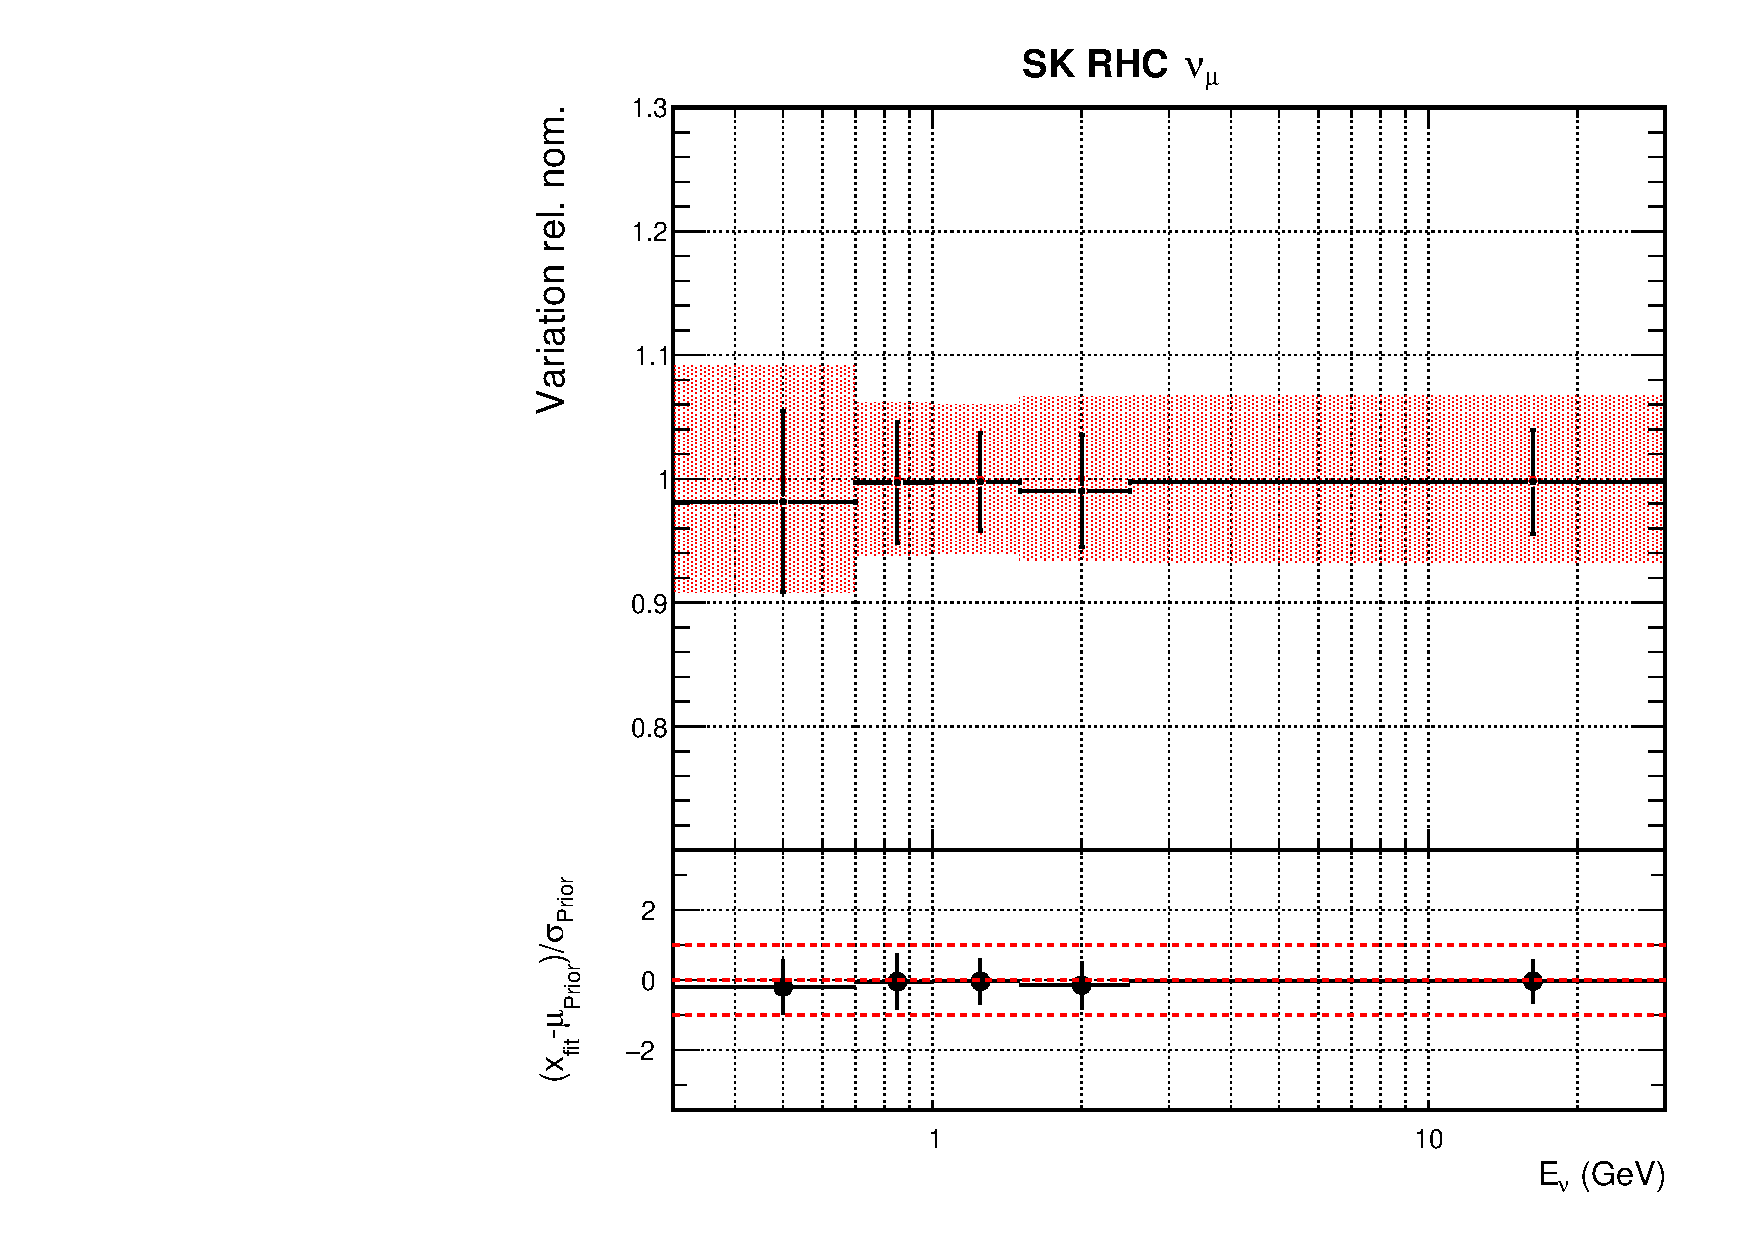
\includegraphics[width=0.75\linewidth]{figs/asmvfluxpoly12}
  \caption{\SK RHC $\nu_{\mu}$}
\end{subfigure}
\begin{subfigure}{0.45\textwidth}
  \centering
  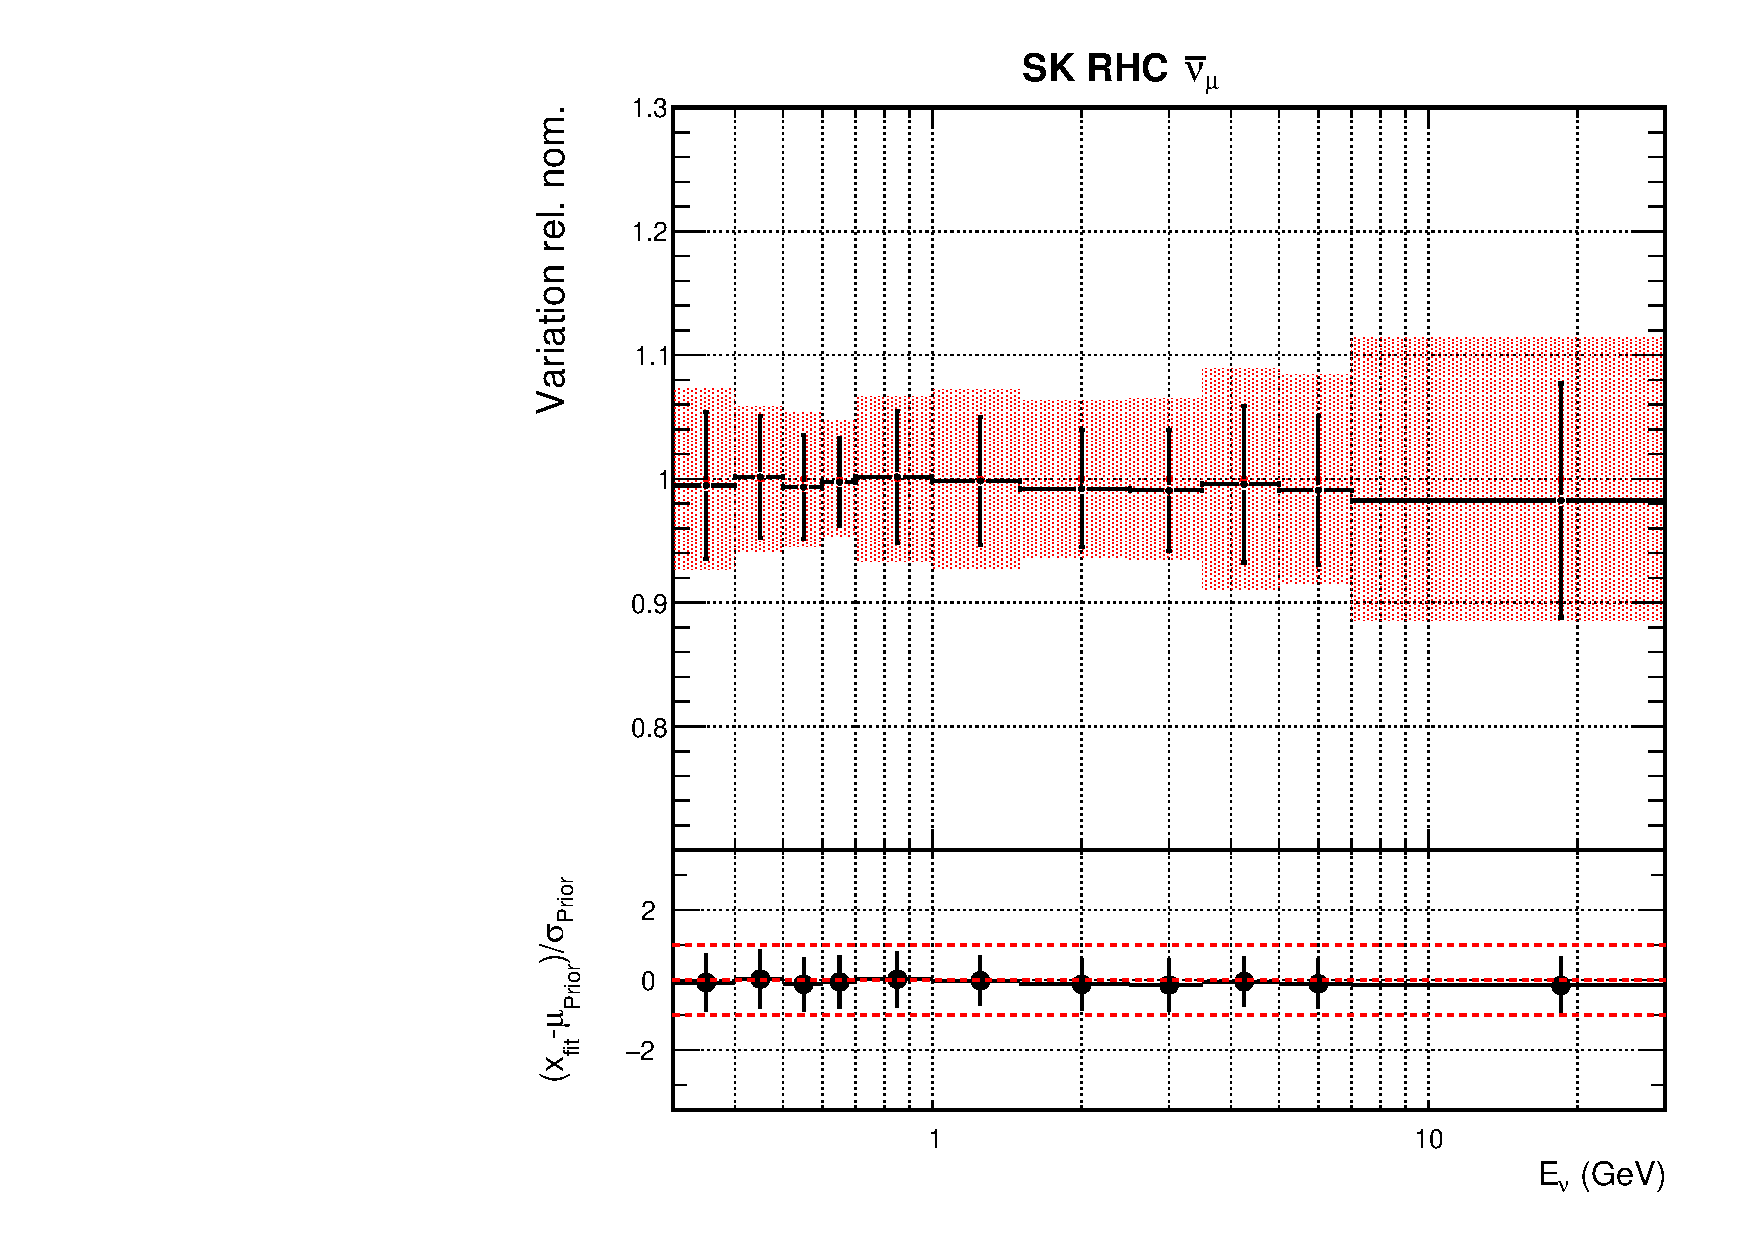
\includegraphics[width=0.75\linewidth]{figs/asmvfluxpoly13}
  \caption{\SK RHC $\bar{\nu_{\mu}}$}
\end{subfigure}
\begin{subfigure}{0.45\textwidth}
  \centering
  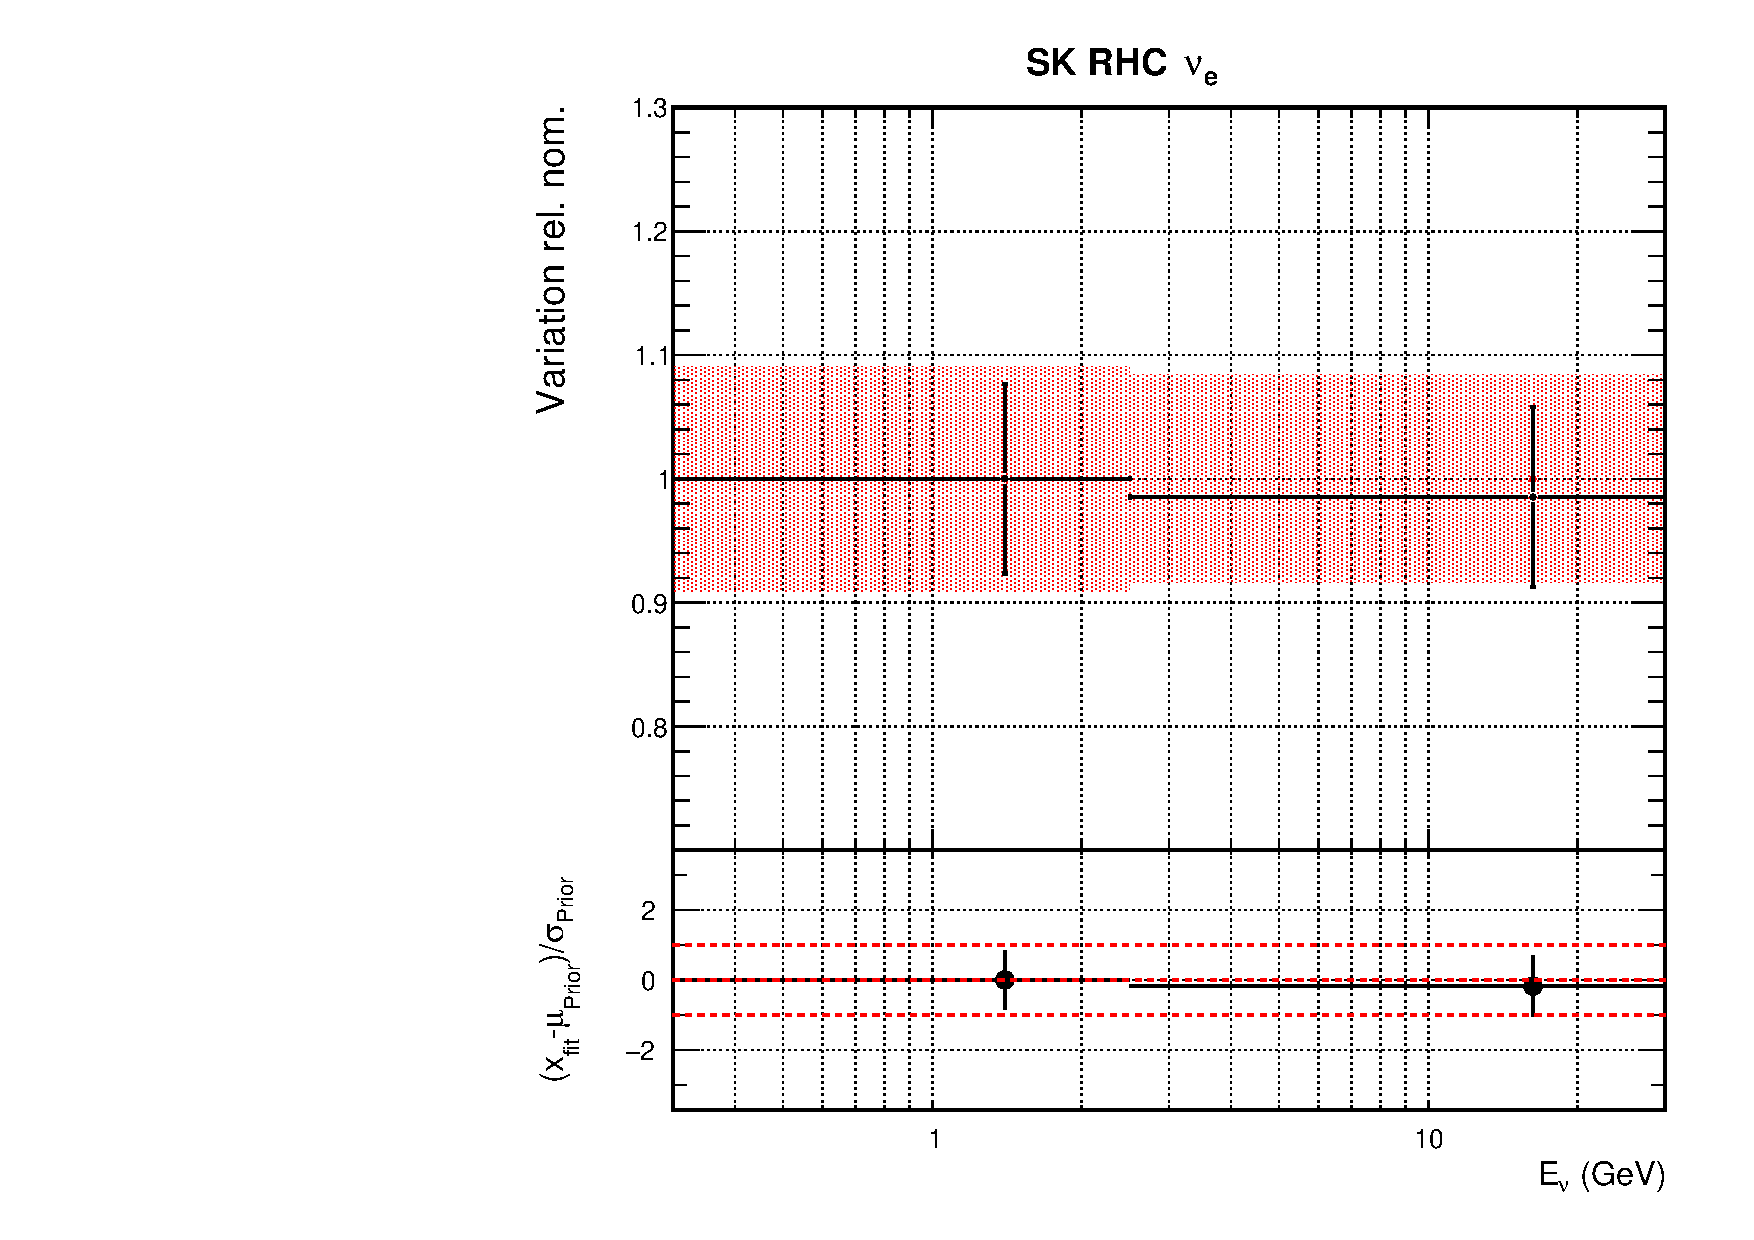
\includegraphics[width=0.75\linewidth]{figs/asmvfluxpoly14}
  \caption{\SK RHC $\nu_{e}$}
\end{subfigure}
\begin{subfigure}{0.45\textwidth}
  \centering
  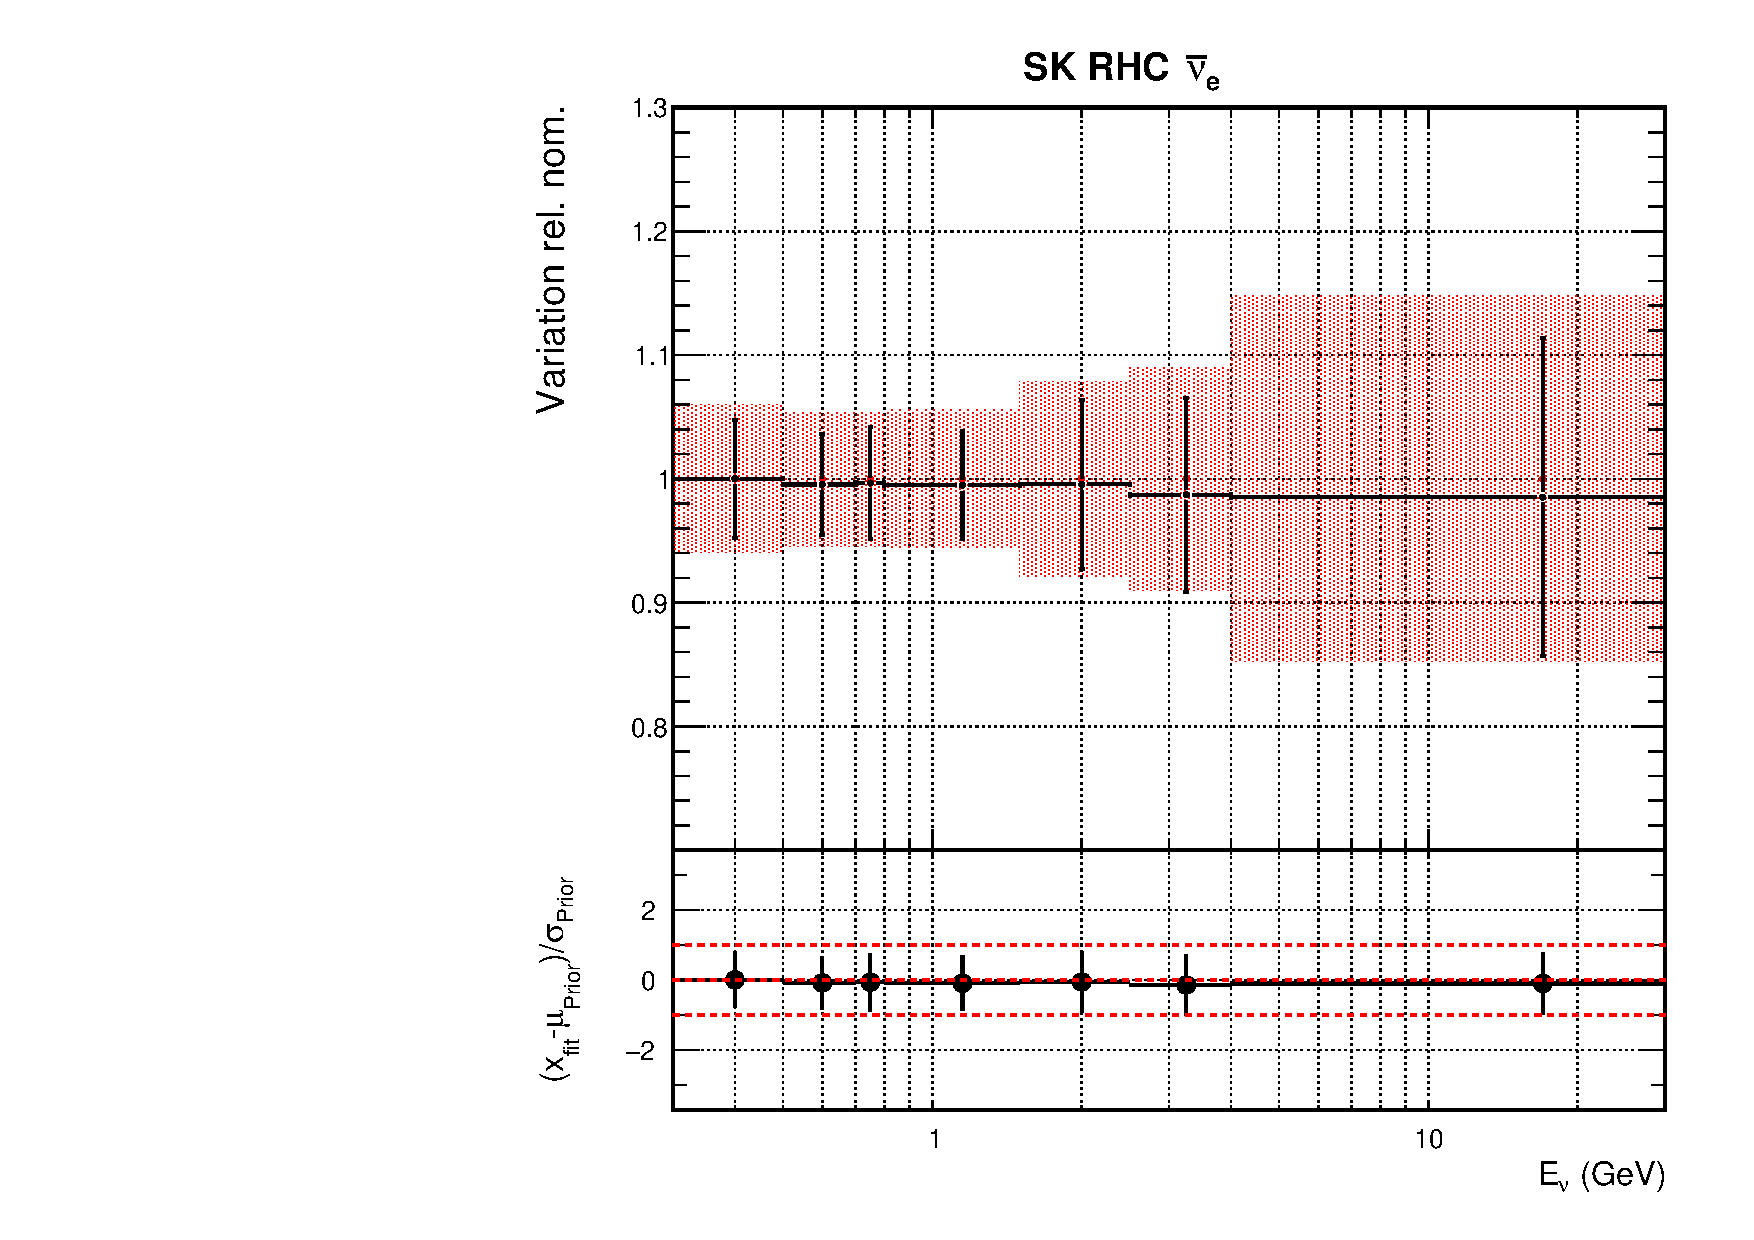
\includegraphics[width=0.75\linewidth]{figs/asmvfluxpoly15}
  \caption{\SK RHC $\bar{\nu_e}$}
\end{subfigure}
\caption{\SK flux parameters for the Asimov fit.}
\label{fig:asmvfluxSKapp}
\end{figure}

\begin{figure}[!htbp]
\centering
\begin{subfigure}{0.8\textwidth}
  \centering
  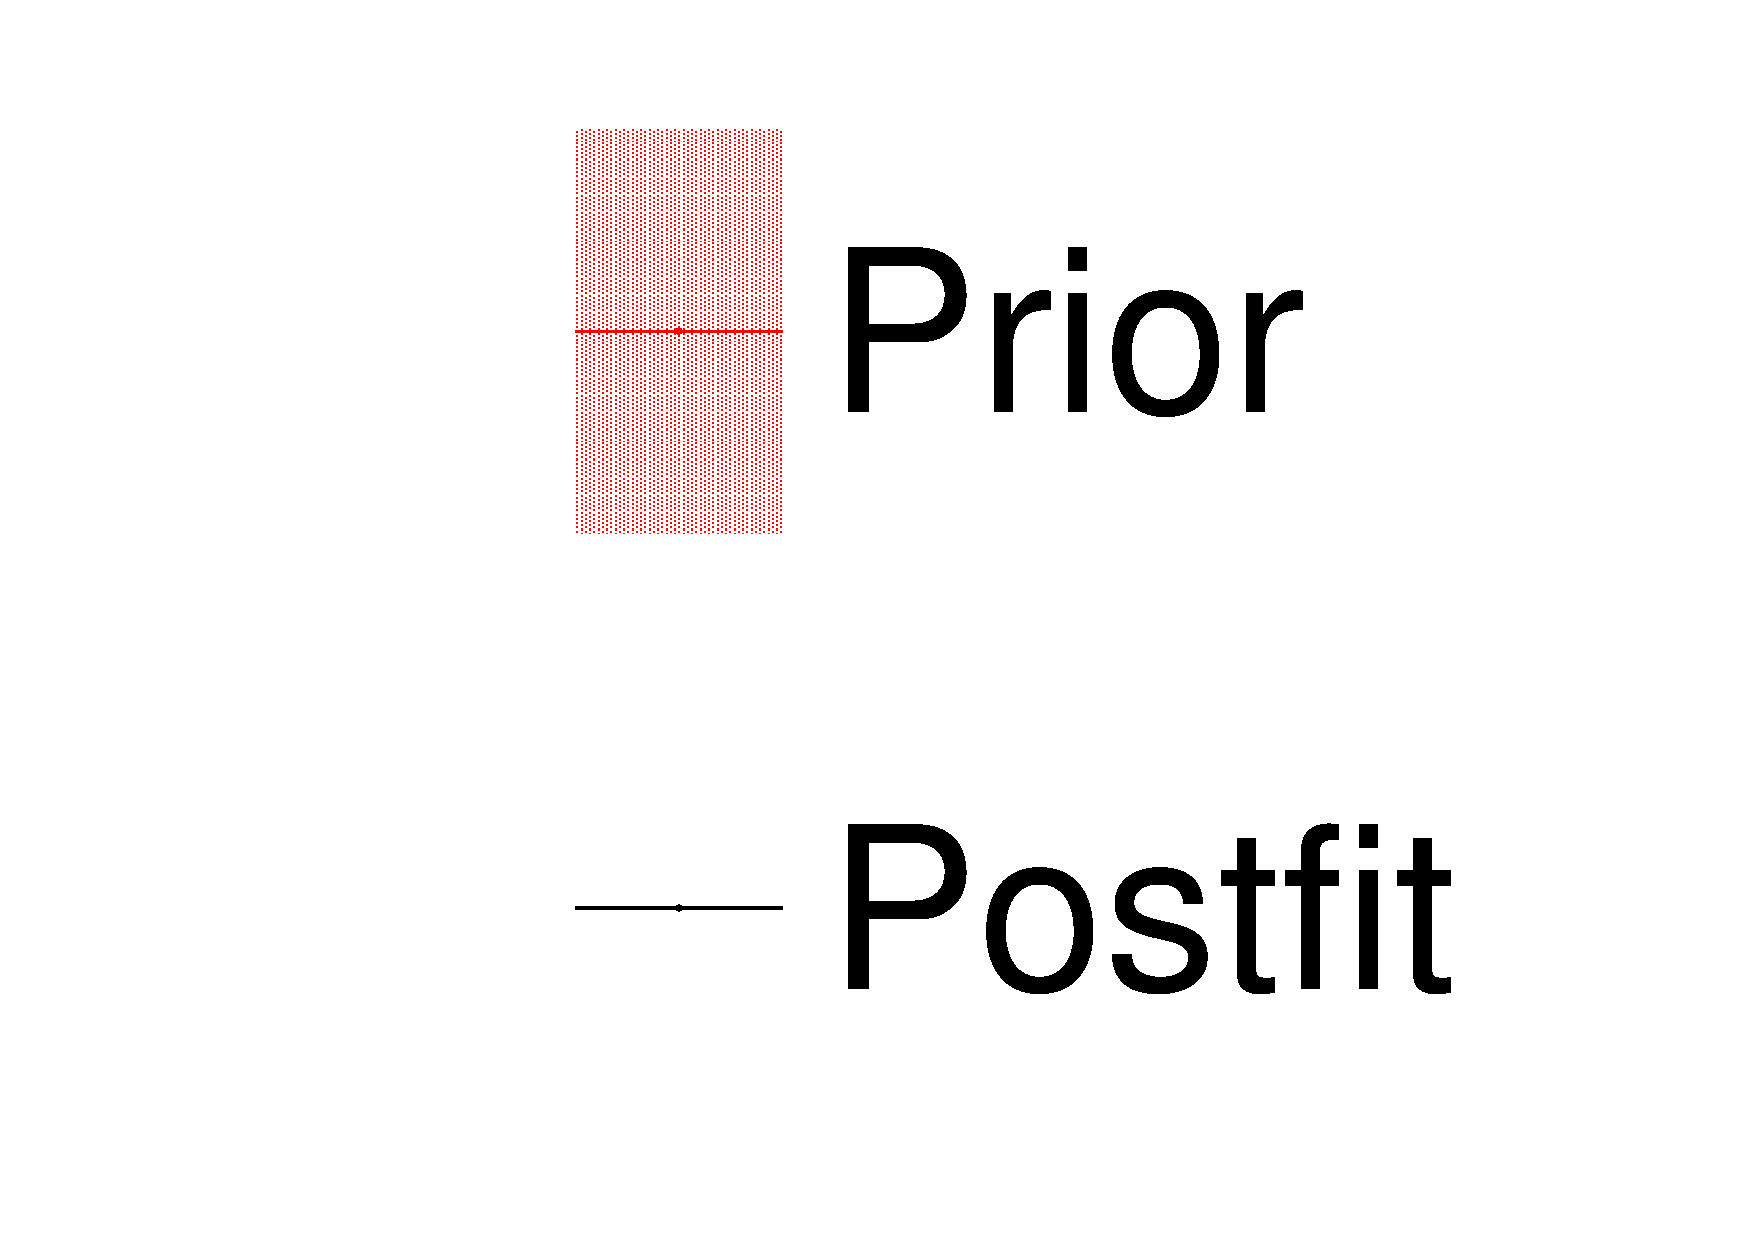
\includegraphics[width=0.25\linewidth]{figs/asmv_leg}
\end{subfigure}
\begin{subfigure}{0.49\textwidth}
  \centering
  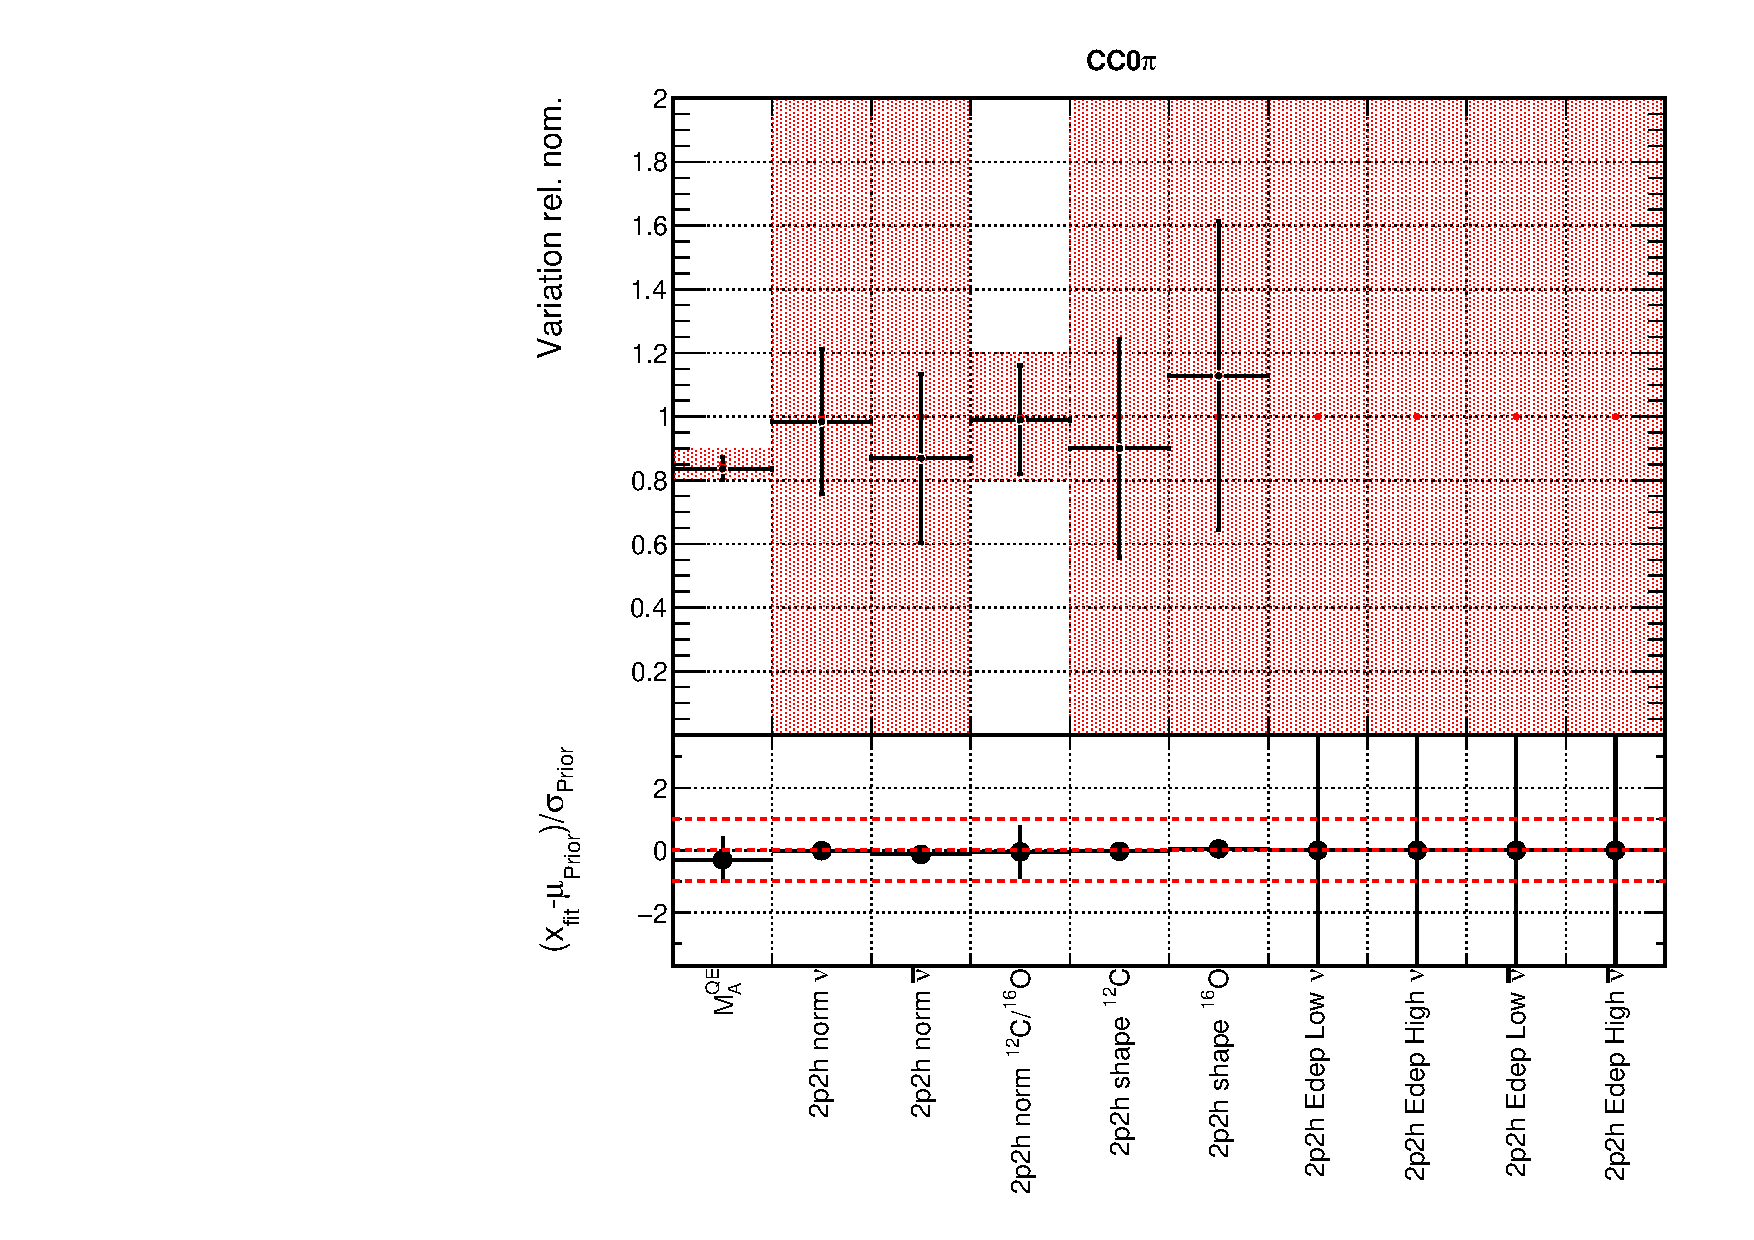
\includegraphics[width=0.9\linewidth]{figs/asmvxsecpoly1}
  \caption{CC 0$\pi$}
\end{subfigure}
\begin{subfigure}{0.49\textwidth}
  \centering
  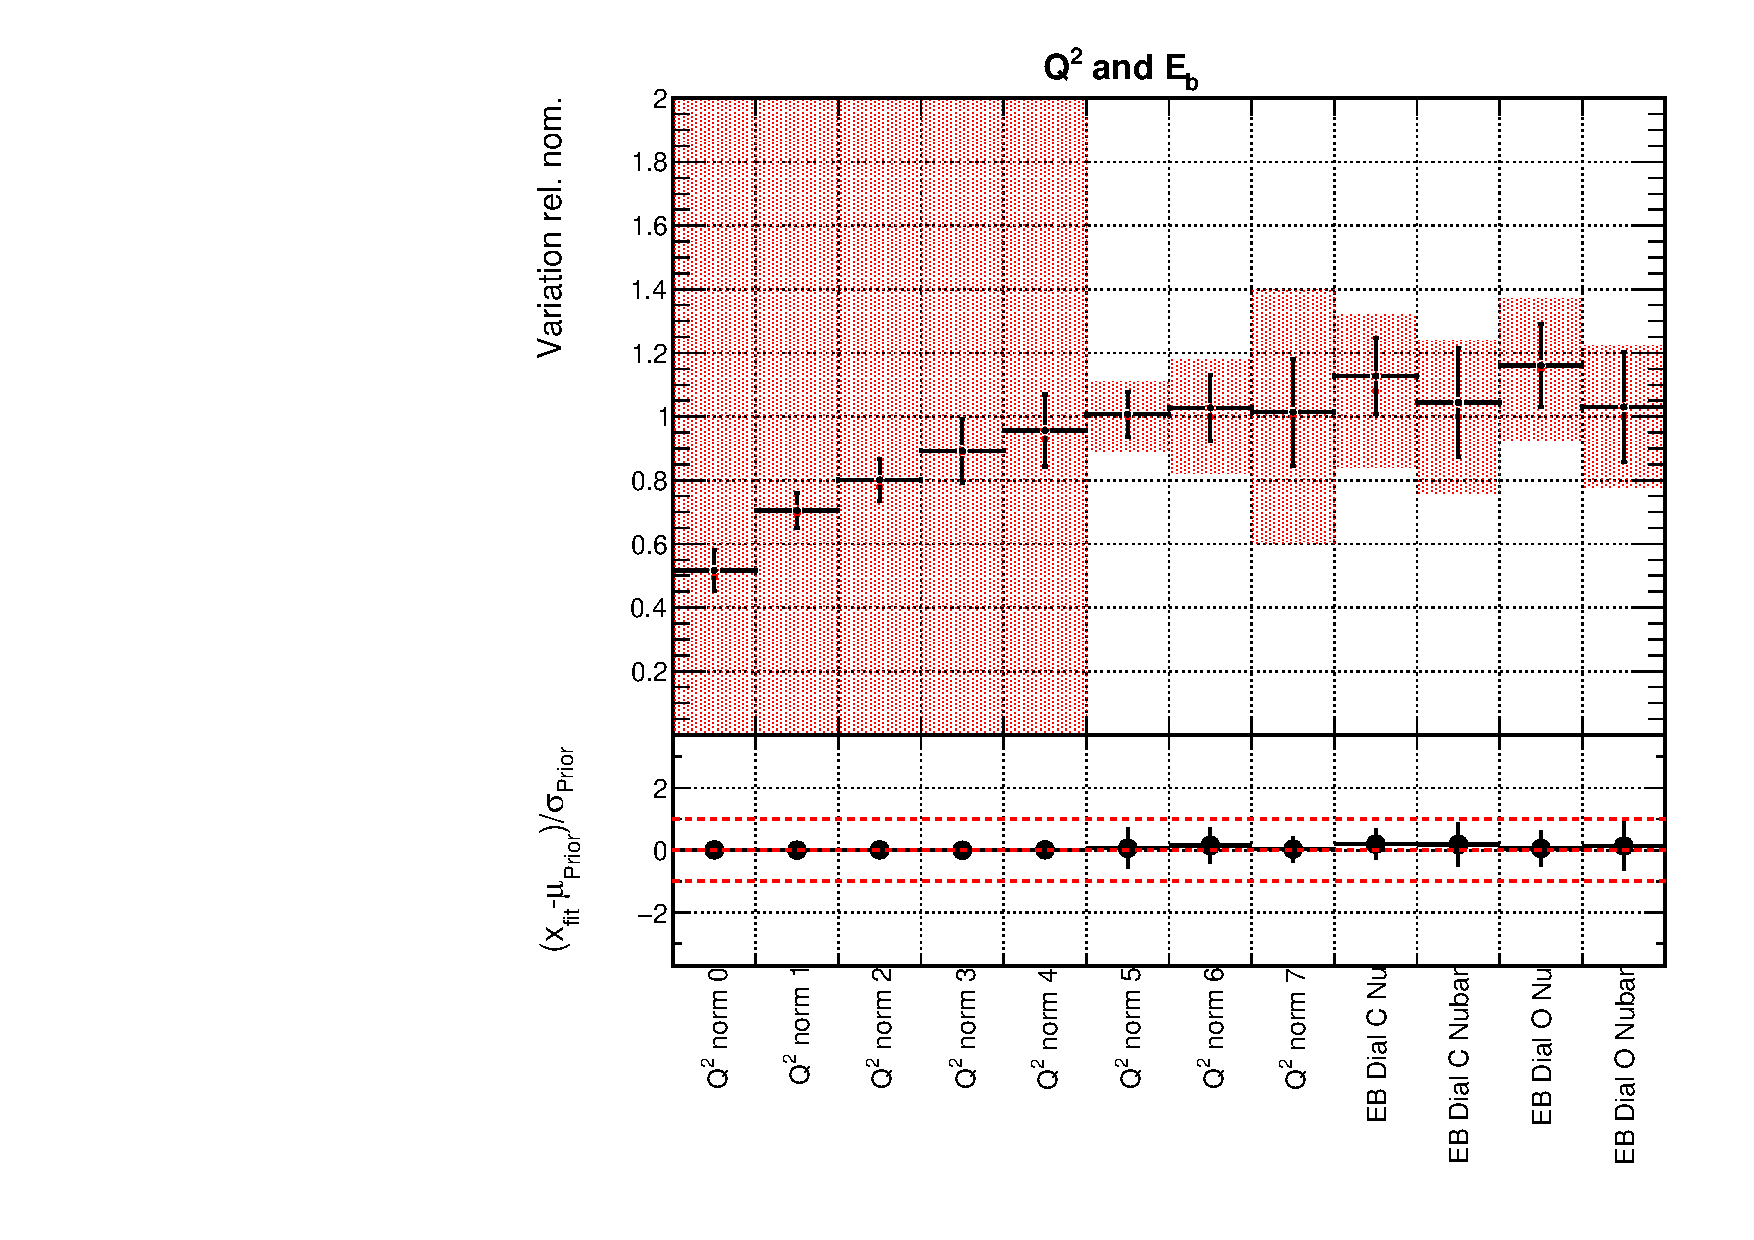
\includegraphics[width=0.9\linewidth]{figs/asmvxsecpoly2}
  \caption{$Q^2$ and $E_{\mathrm{b}}$}
\end{subfigure}
\begin{subfigure}{0.49\textwidth}
  \centering
  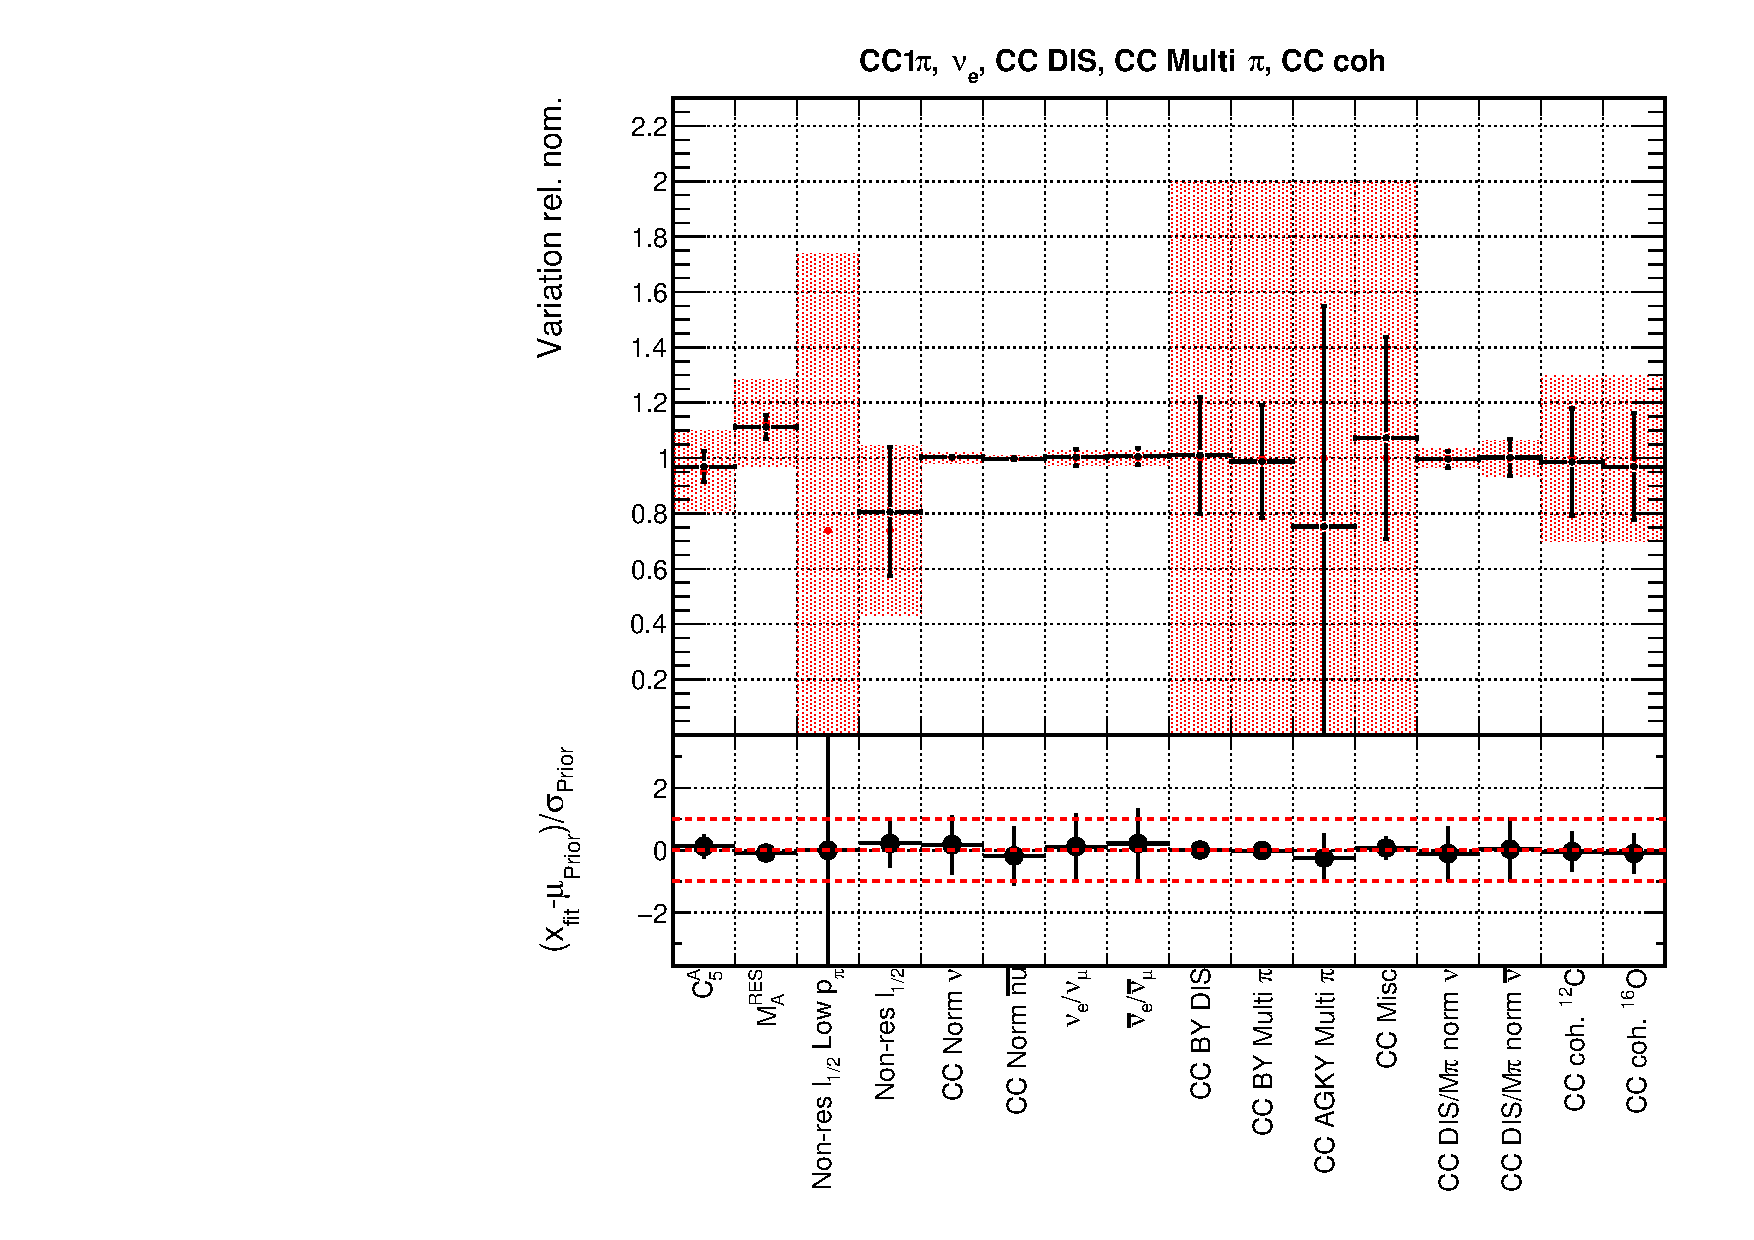
\includegraphics[width=0.9\linewidth]{figs/asmvxsecpoly3}
  \caption{CC 1$\pi$, $\nu_e$, CC DIS, CC multi-$\pi$ and CC Coh.}
\end{subfigure}
\begin{subfigure}{0.49\textwidth}
  \centering
  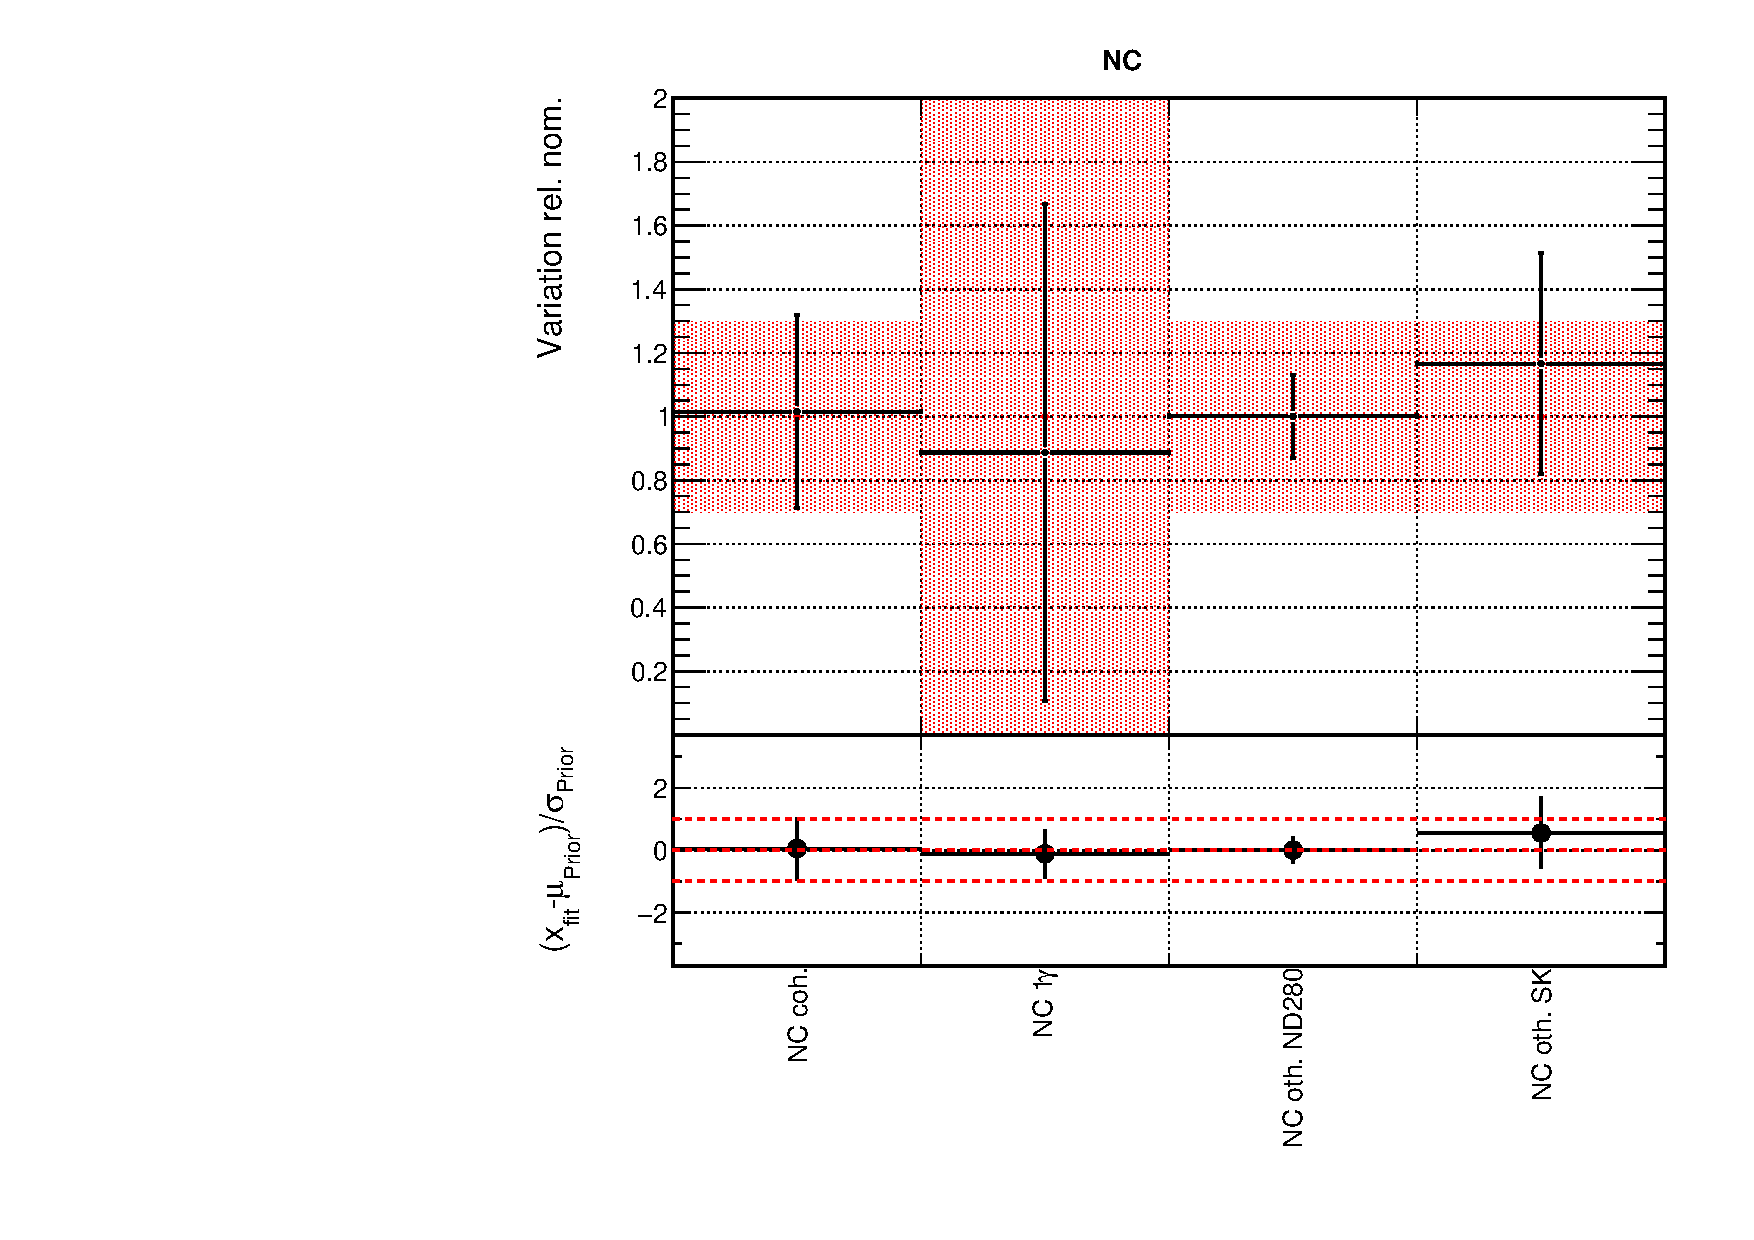
\includegraphics[width=0.9\linewidth]{figs/asmvxsecpoly4}
  \caption{NC}
\end{subfigure}
\begin{subfigure}{0.49\textwidth}
  \centering
  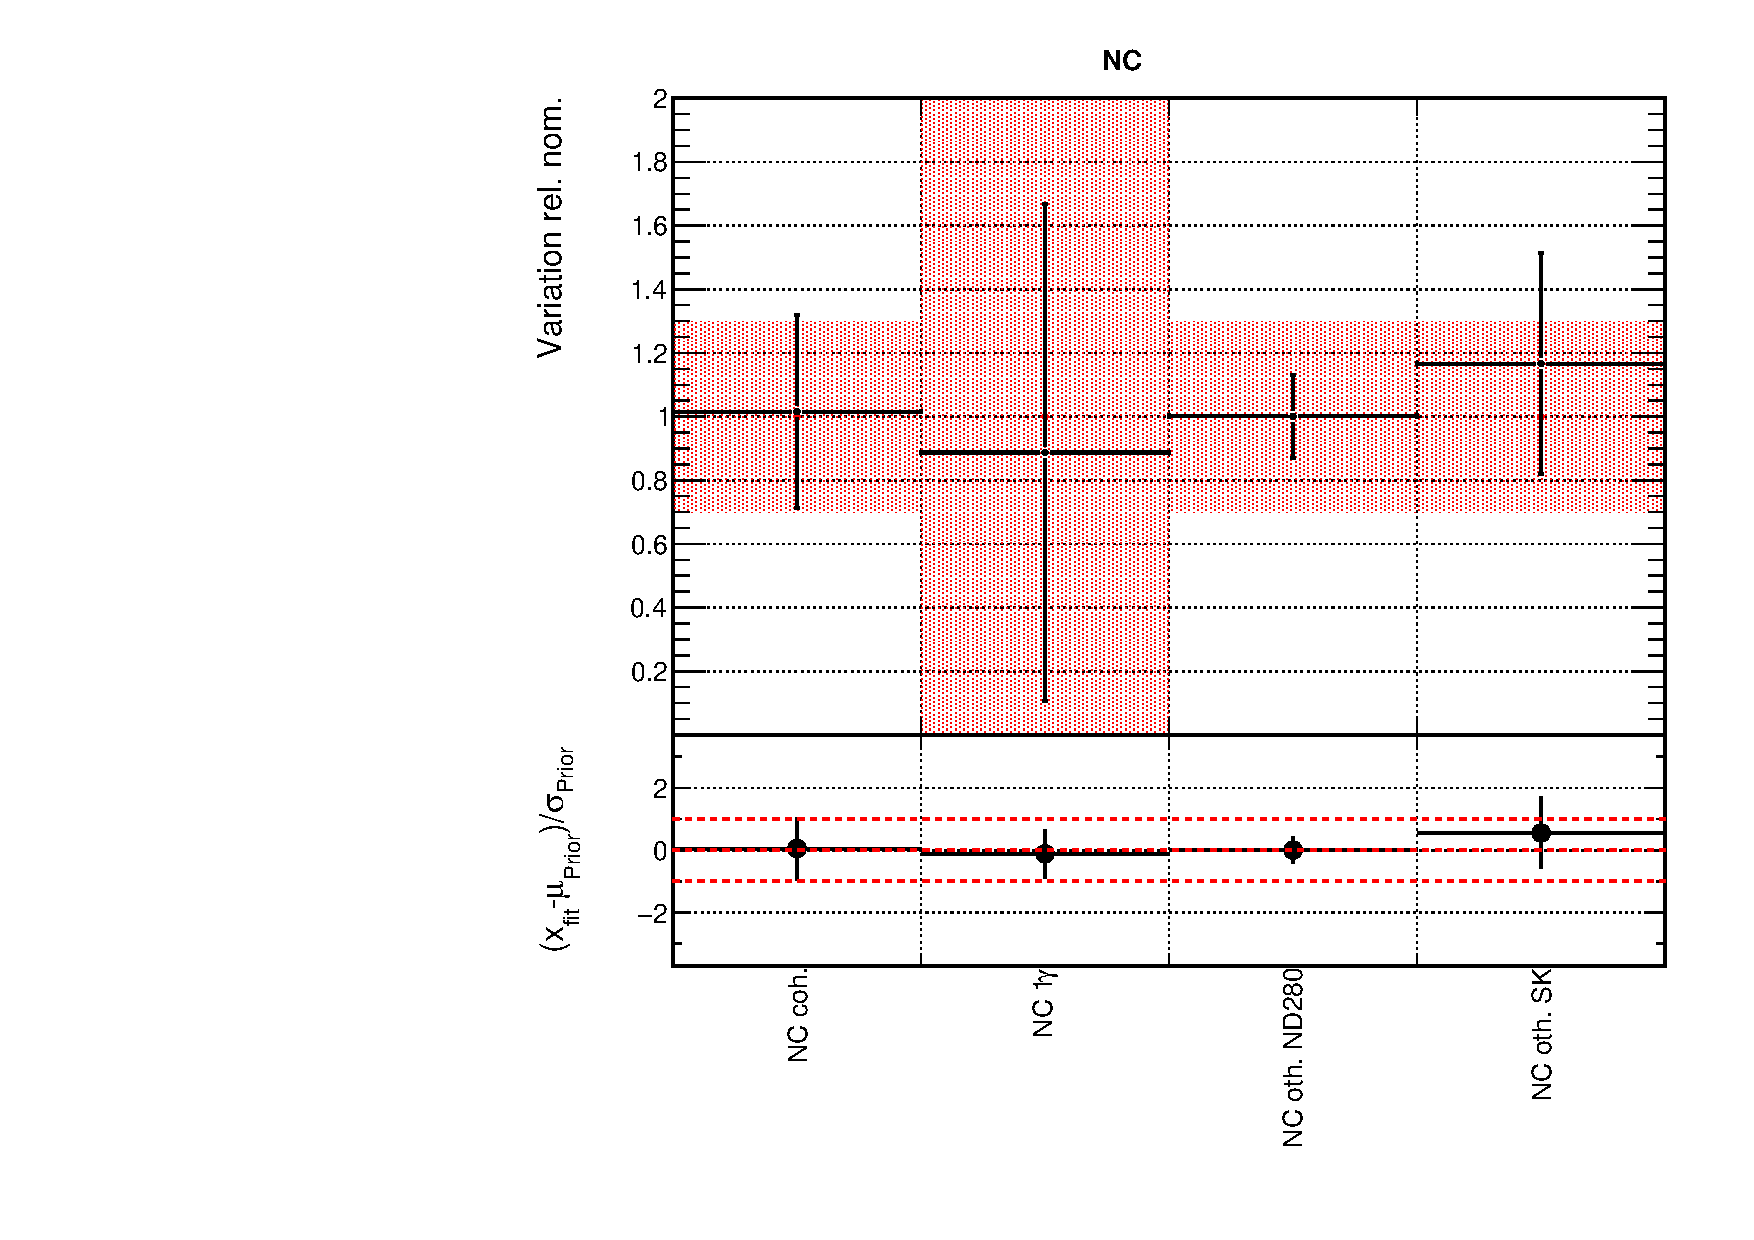
\includegraphics[width=0.9\linewidth]{figs/asmvxsecpoly4}
  \caption{$\pi$ FSI}
\end{subfigure}
\caption{Interaction parameters for the Asimov fit.}
\label{fig:asmvxsecapp}
\end{figure}

The results for the data fit are shown in Figures \ref{fig:datfluxNDapp}, \ref{fig:datfluxSKapp} and \ref{fig:datxsecapp}.

\begin{figure}[!htbp]
\centering
\begin{subfigure}{0.8\textwidth}
  \centering
  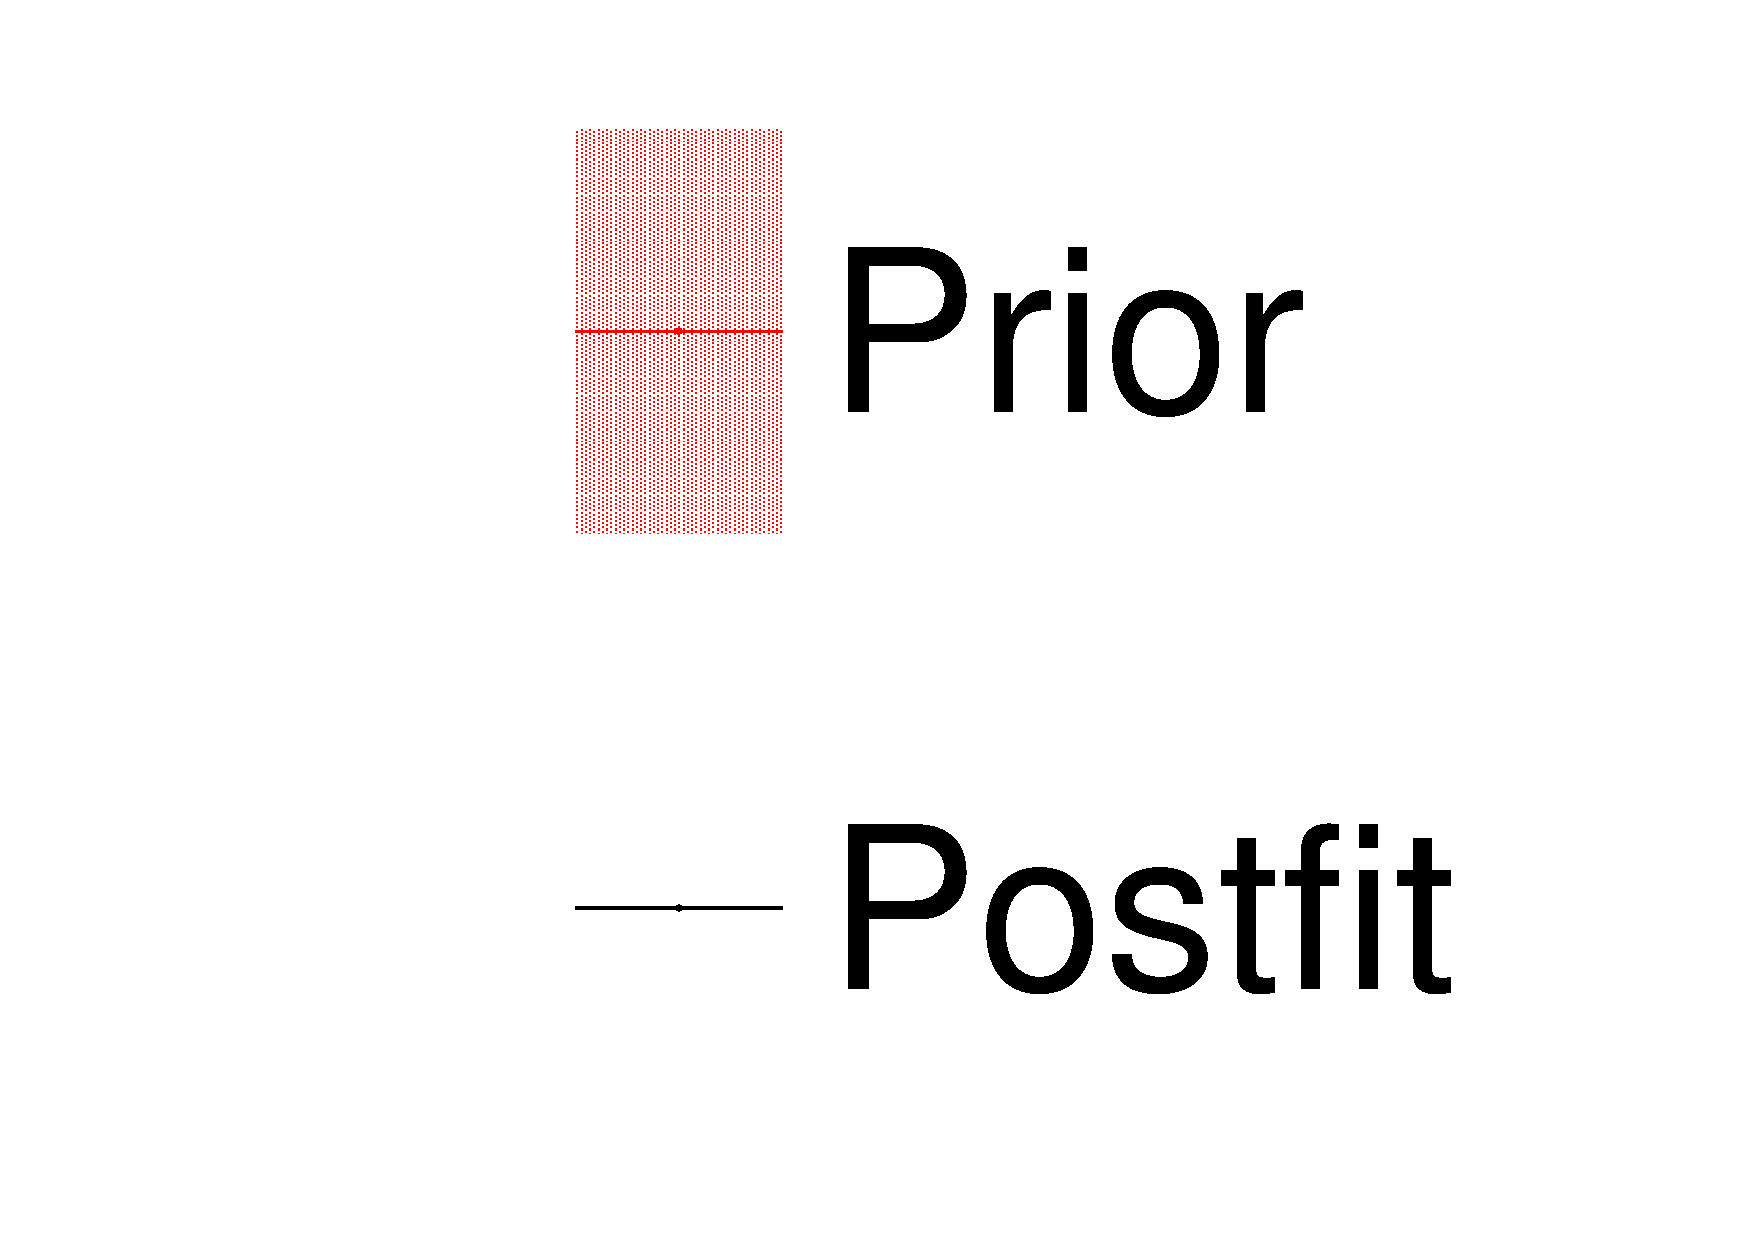
\includegraphics[width=0.24\linewidth]{figs/dat_leg}
\end{subfigure}
\begin{subfigure}{0.45\textwidth}
  \centering
  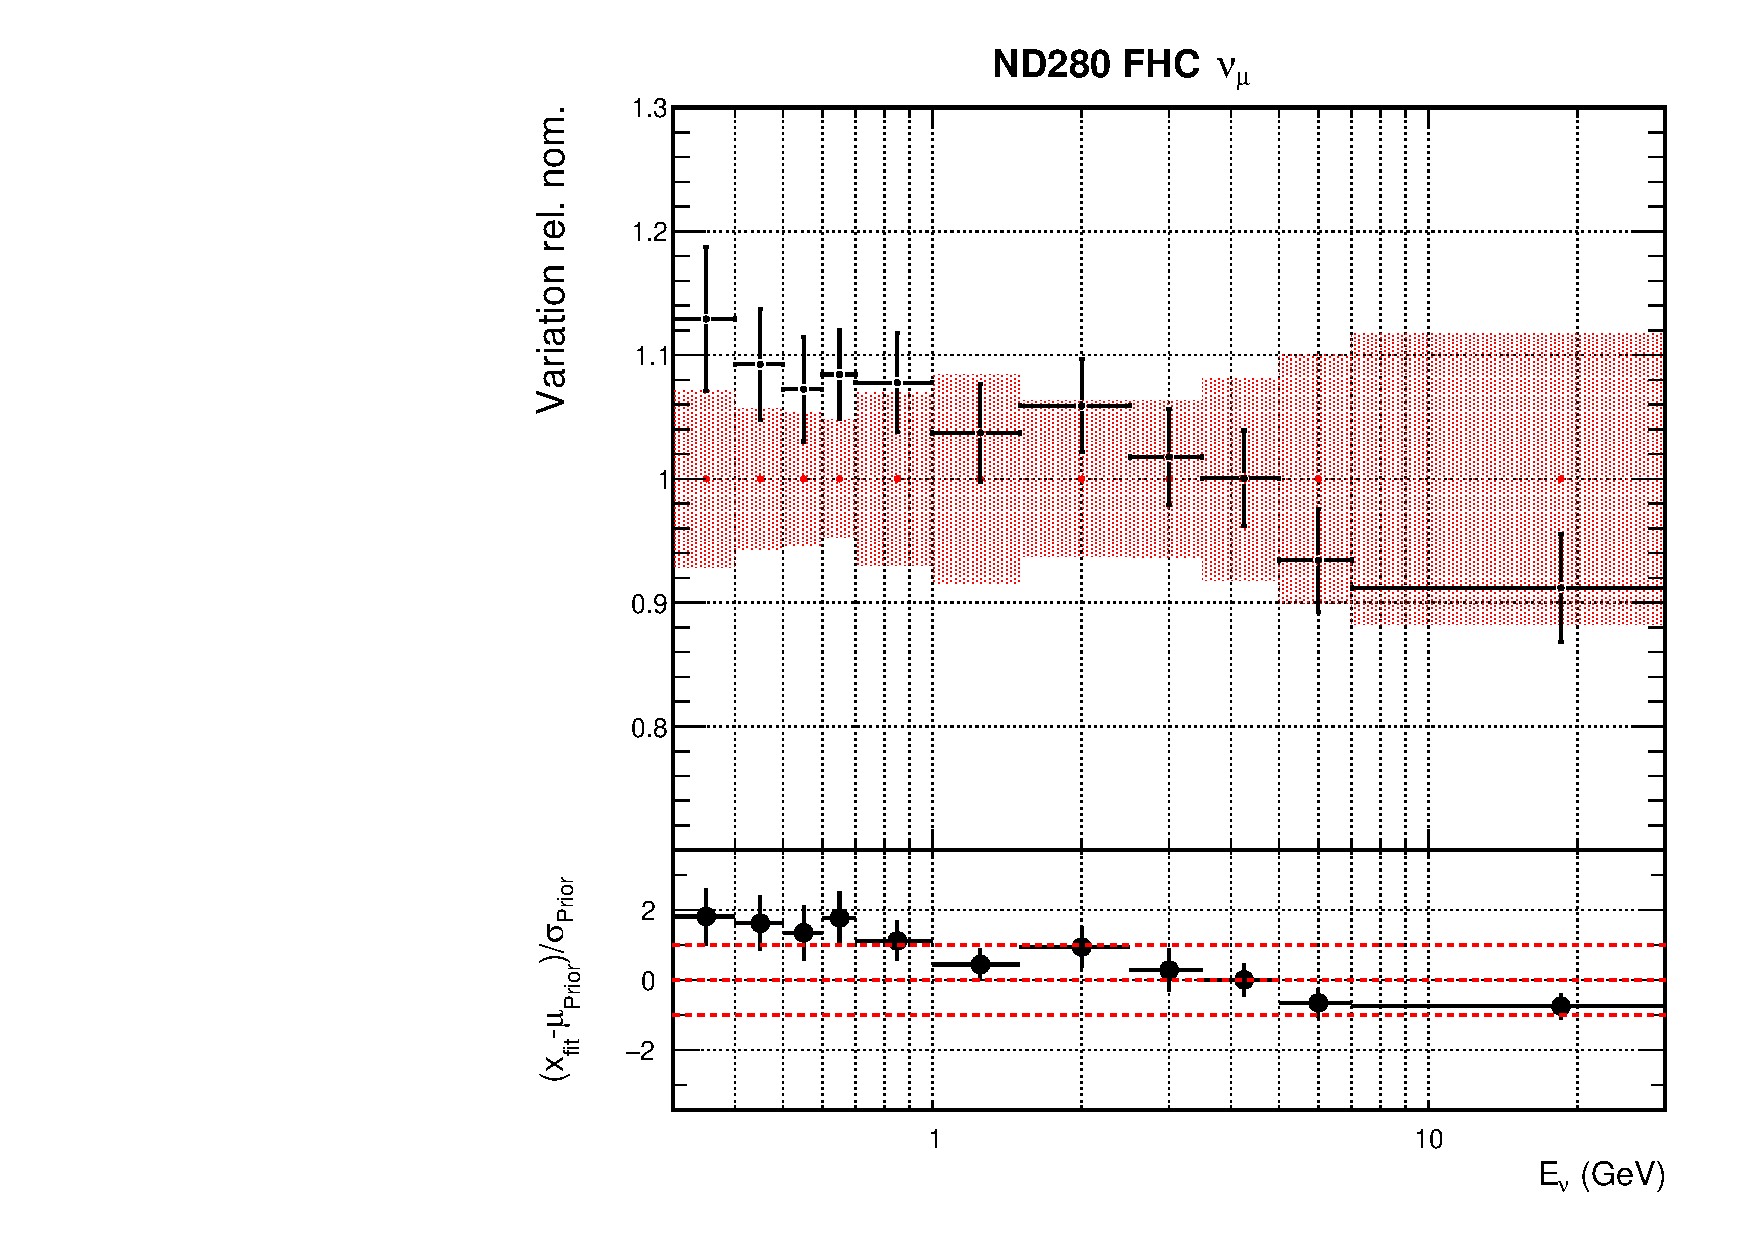
\includegraphics[width=0.75\linewidth]{figs/datflux0}
  \caption{ND FHC $\nu_{\mu}$}
\end{subfigure}
\begin{subfigure}{0.45\textwidth}
  \centering
  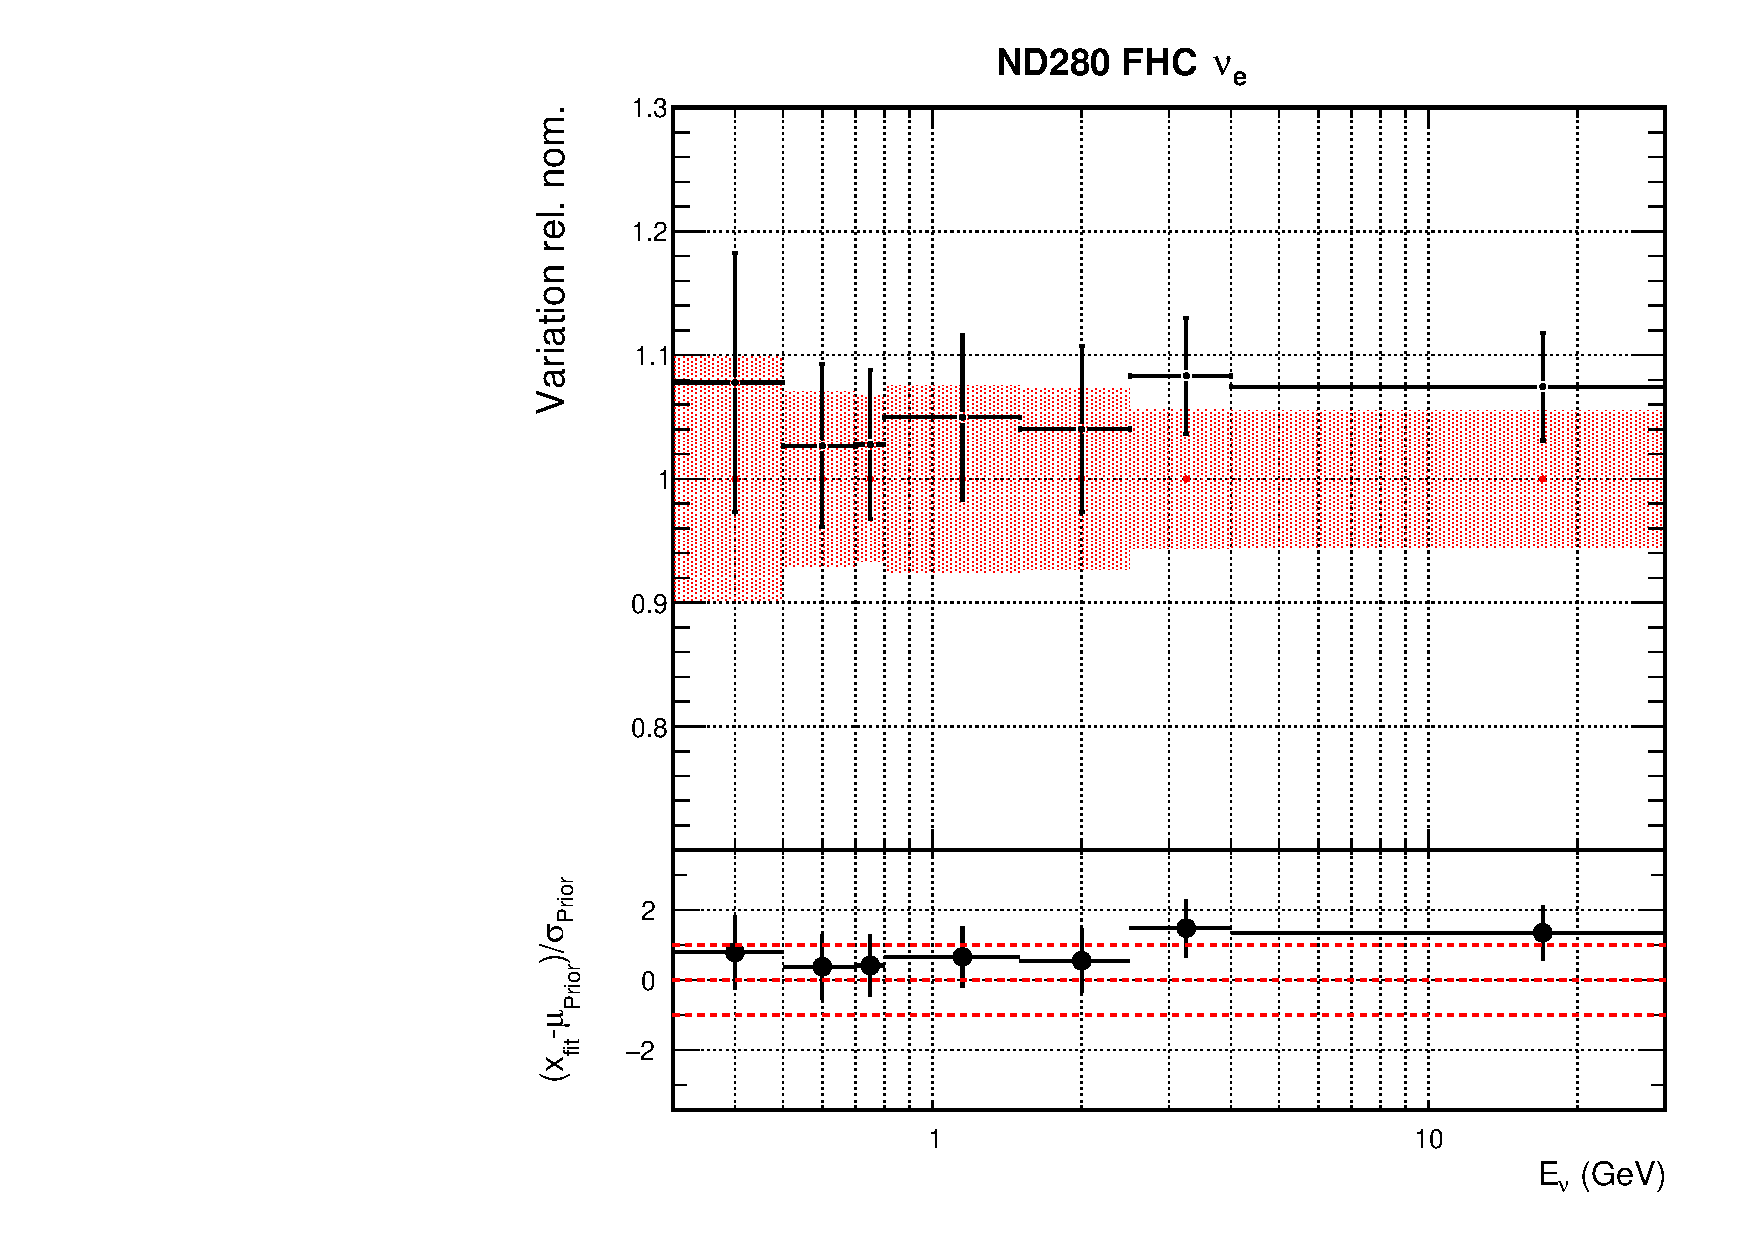
\includegraphics[width=0.75\linewidth]{figs/datflux1}
  \caption{ND FHC $\bar{\nu_{\mu}}$}
\end{subfigure}
\begin{subfigure}{0.45\textwidth}
  \centering
  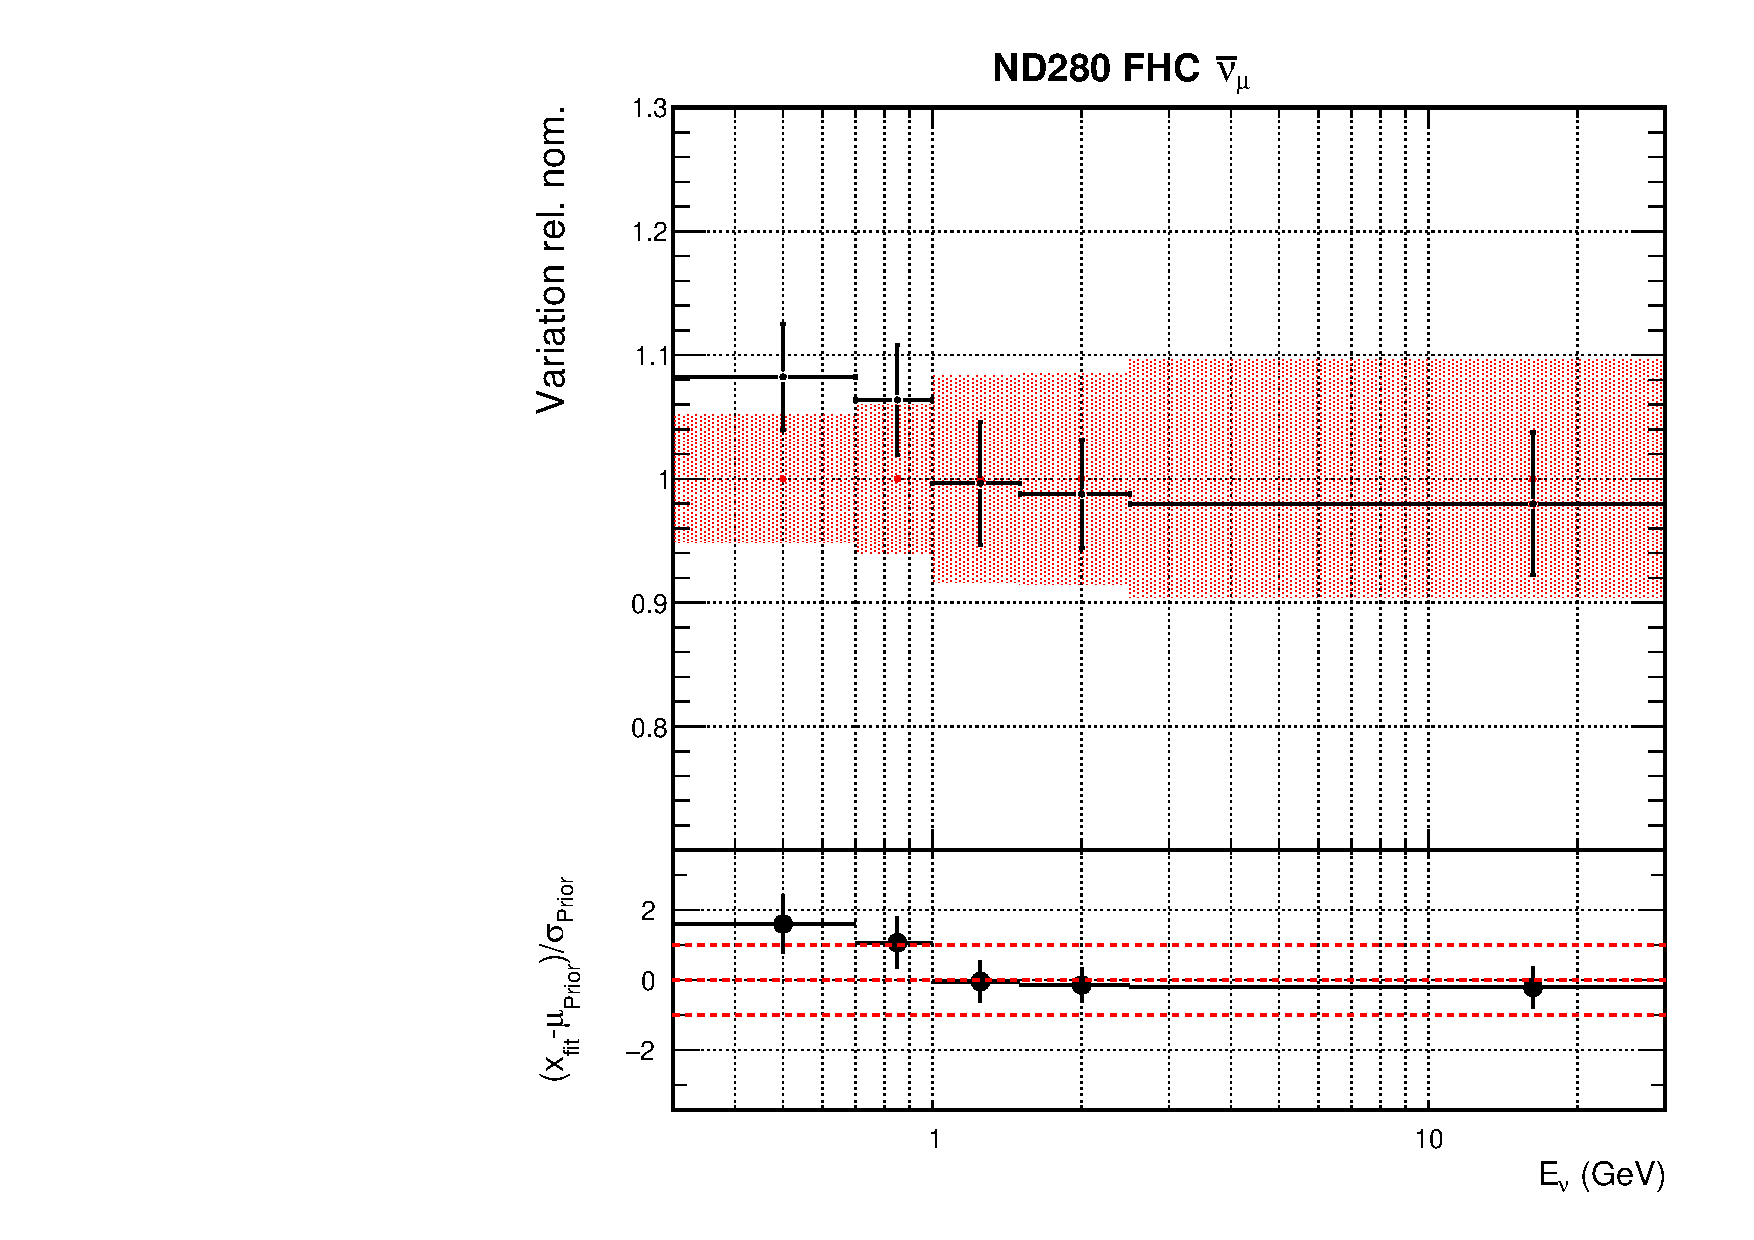
\includegraphics[width=0.75\linewidth]{figs/datflux2}
  \caption{ND FHC $\nu_{e}$}
\end{subfigure}
\begin{subfigure}{0.45\textwidth}
  \centering
  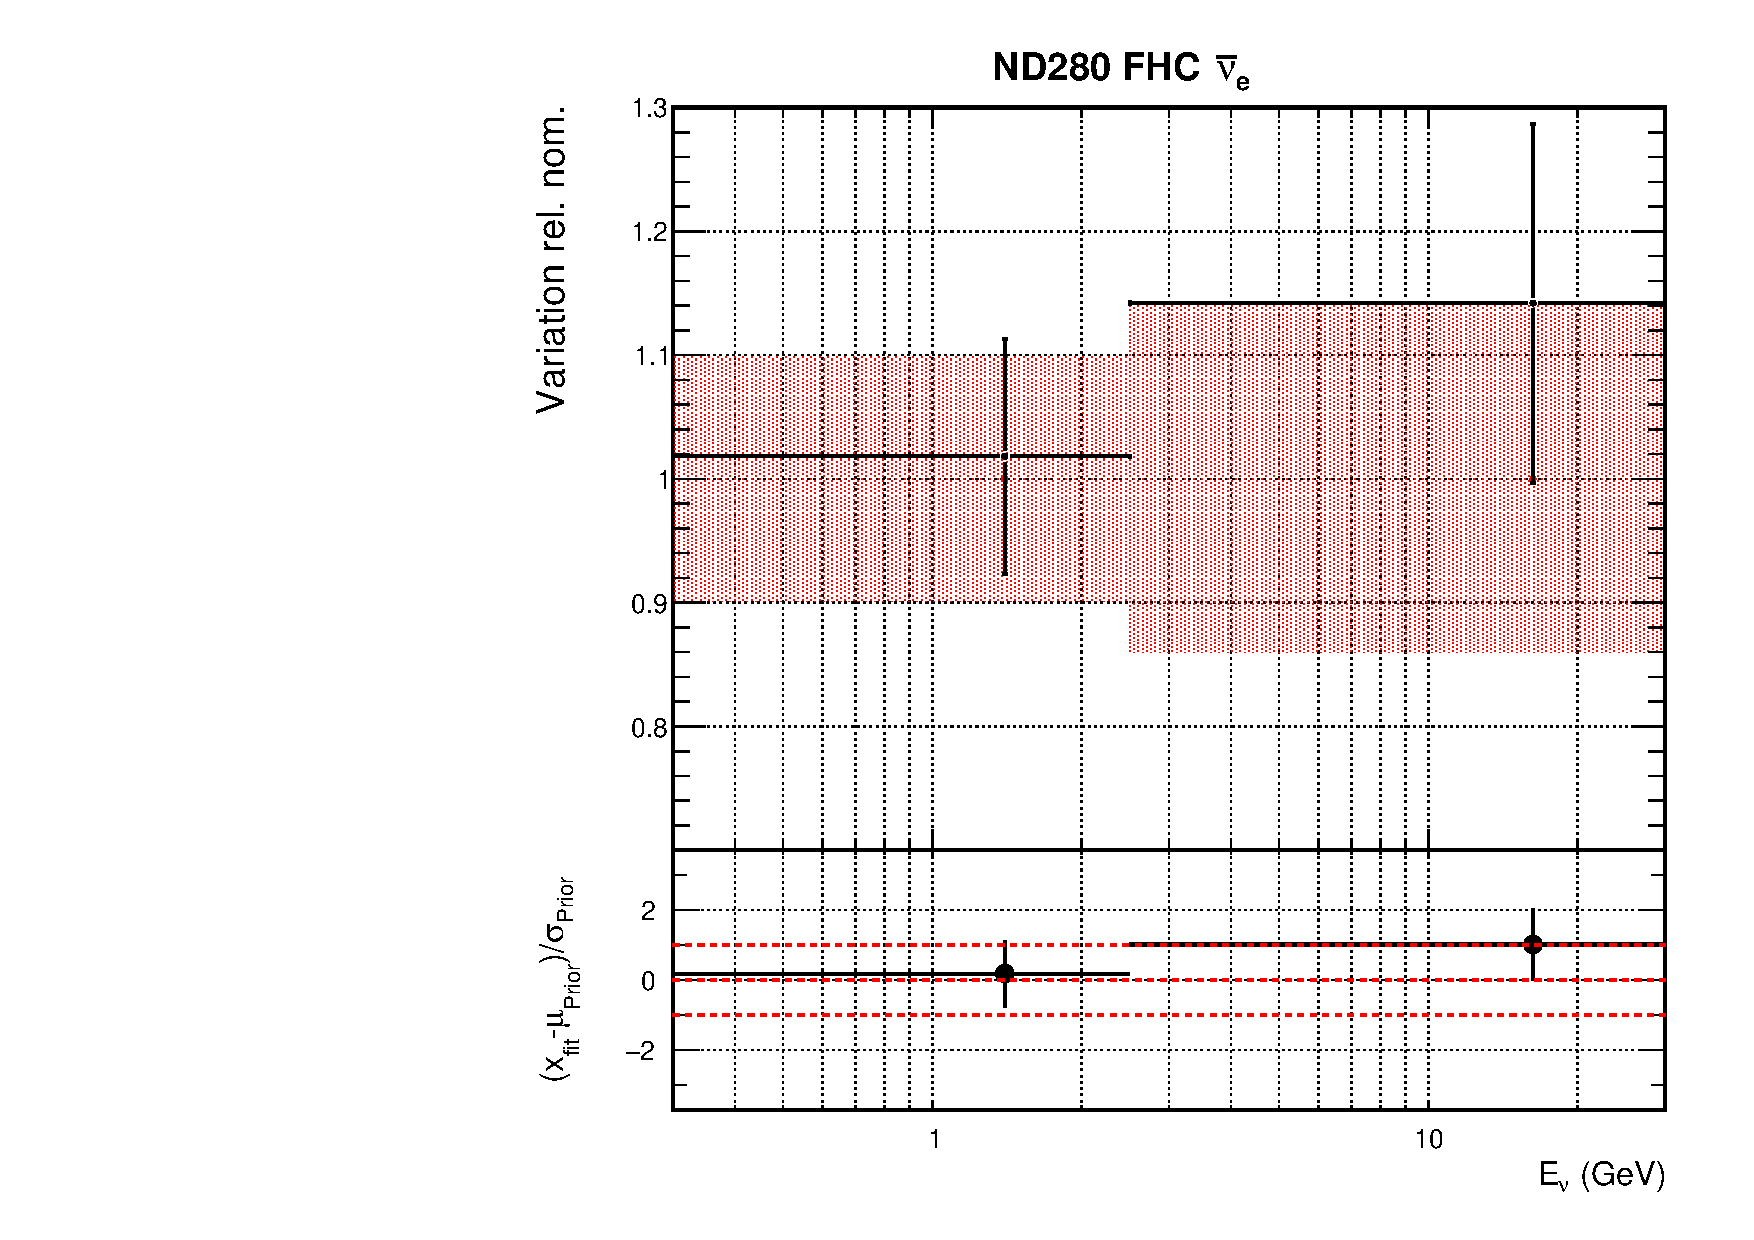
\includegraphics[width=0.75\linewidth]{figs/datflux3}
  \caption{ND FHC $\bar{\nu_{e}}$}
\end{subfigure}
\begin{subfigure}{0.45\textwidth}
  \centering
  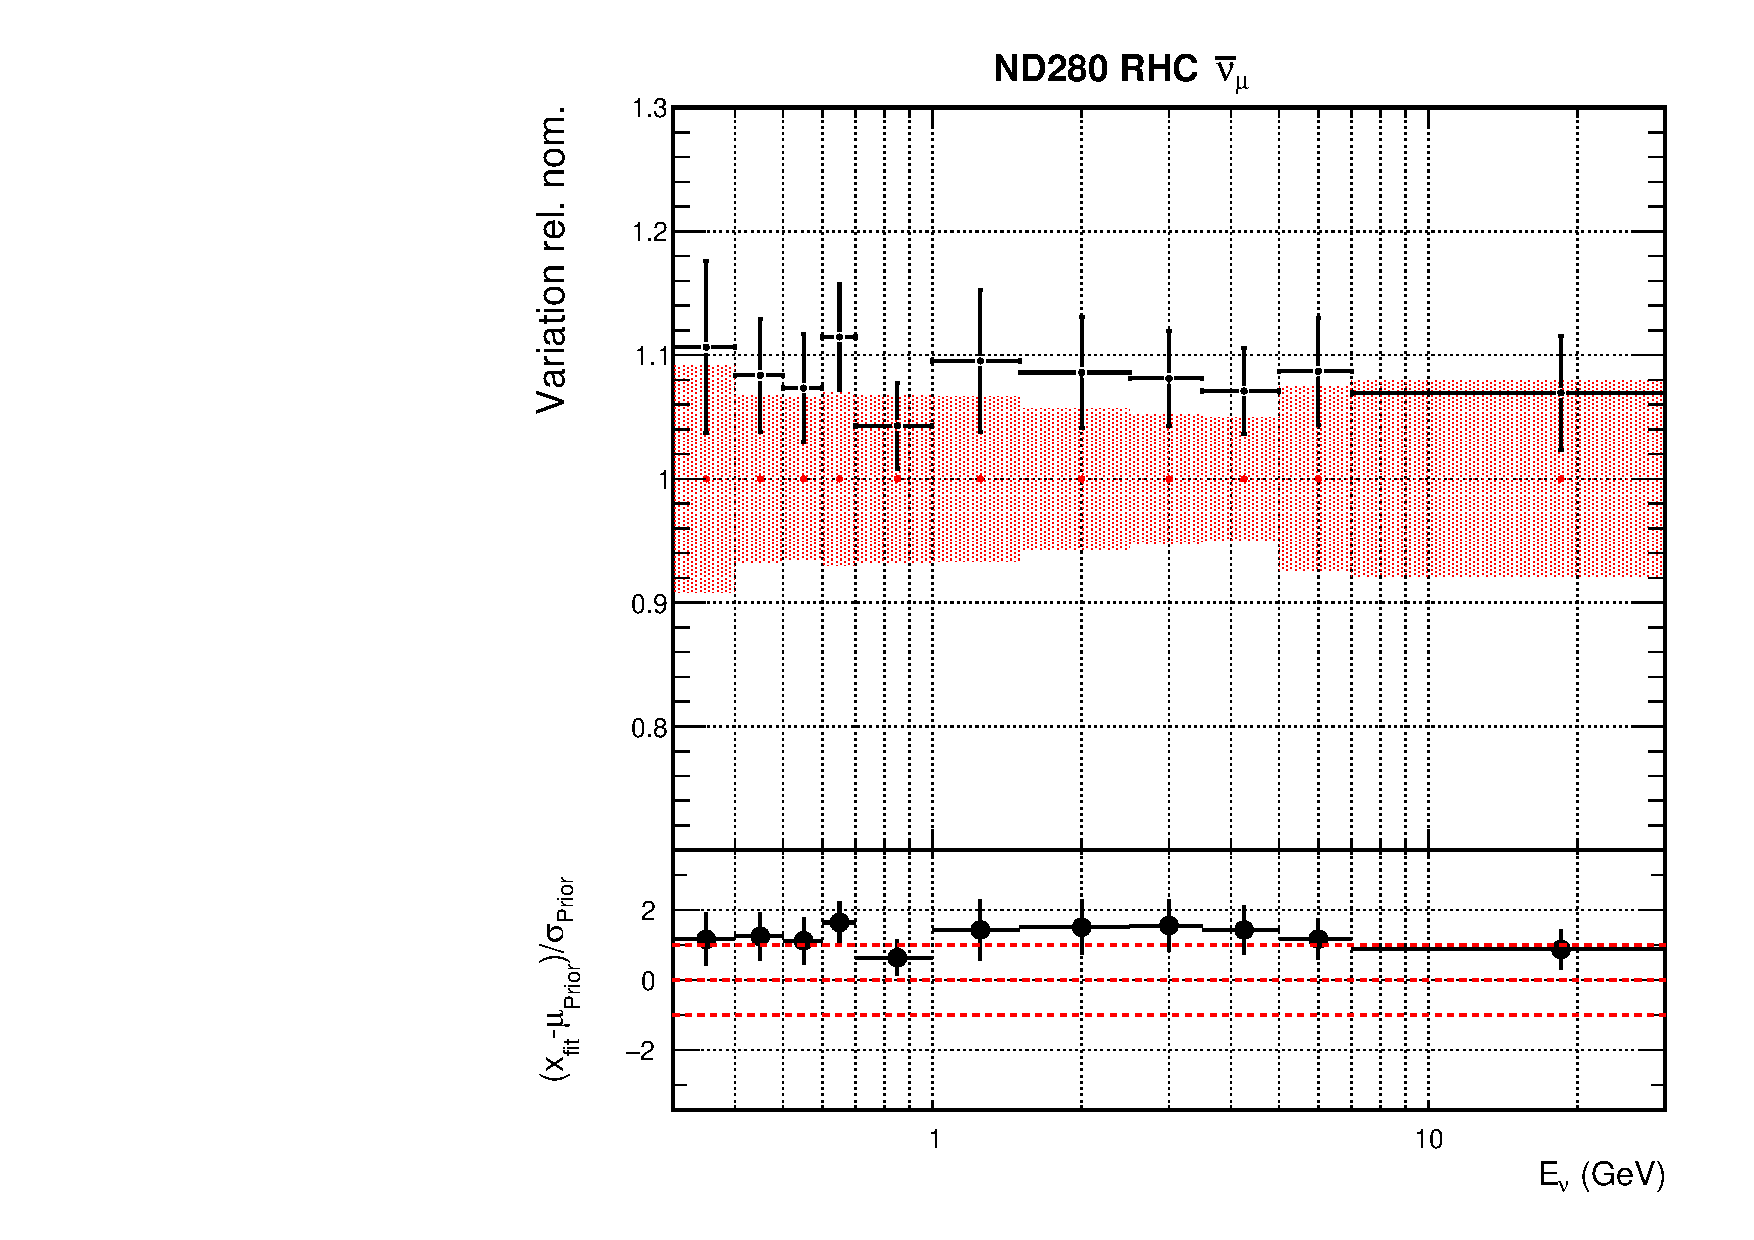
\includegraphics[width=0.75\linewidth]{figs/datflux4}
  \caption{ND RHC $\nu_{\mu}$}
\end{subfigure}
\begin{subfigure}{0.45\textwidth}
  \centering
  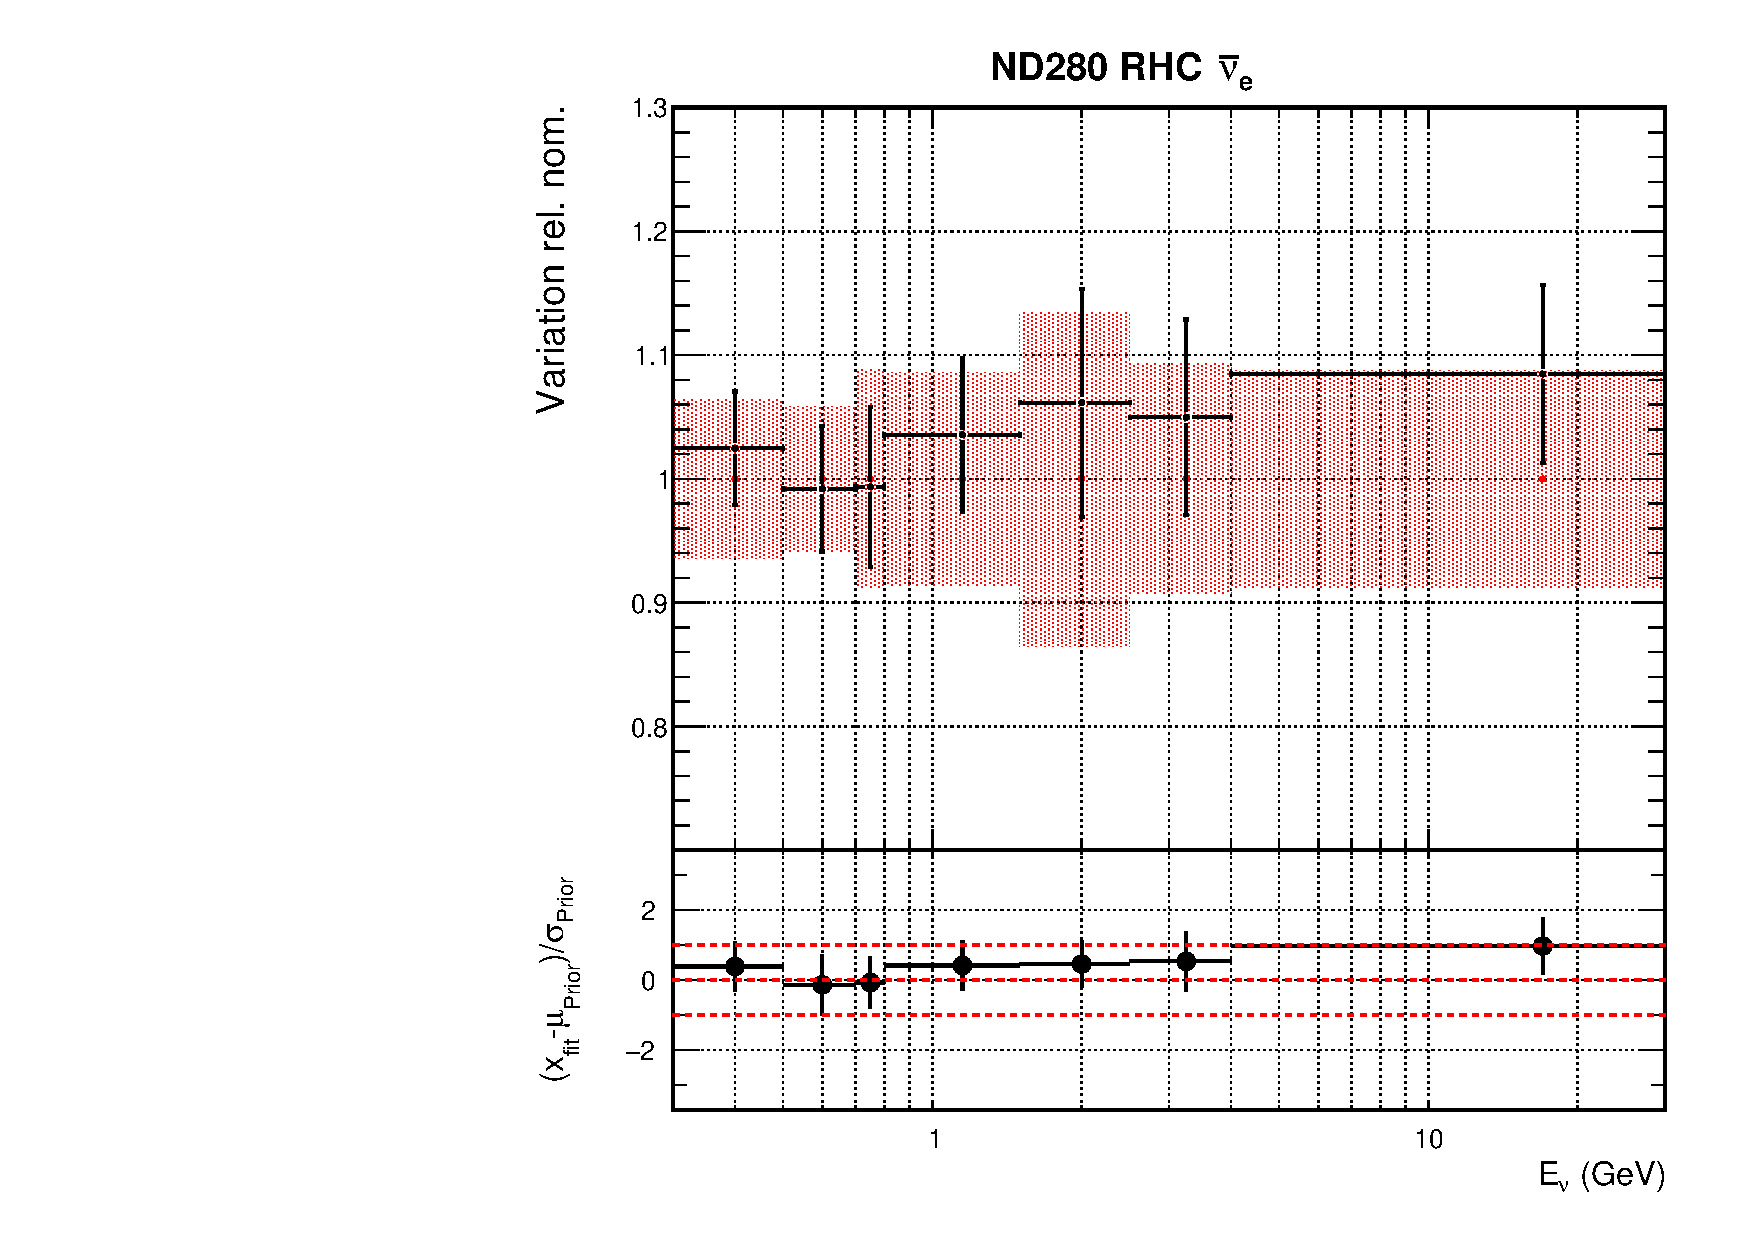
\includegraphics[width=0.75\linewidth]{figs/datflux5}
  \caption{ND RHC $\bar{\nu_{\mu}}$}
\end{subfigure}
\begin{subfigure}{0.45\textwidth}
  \centering
  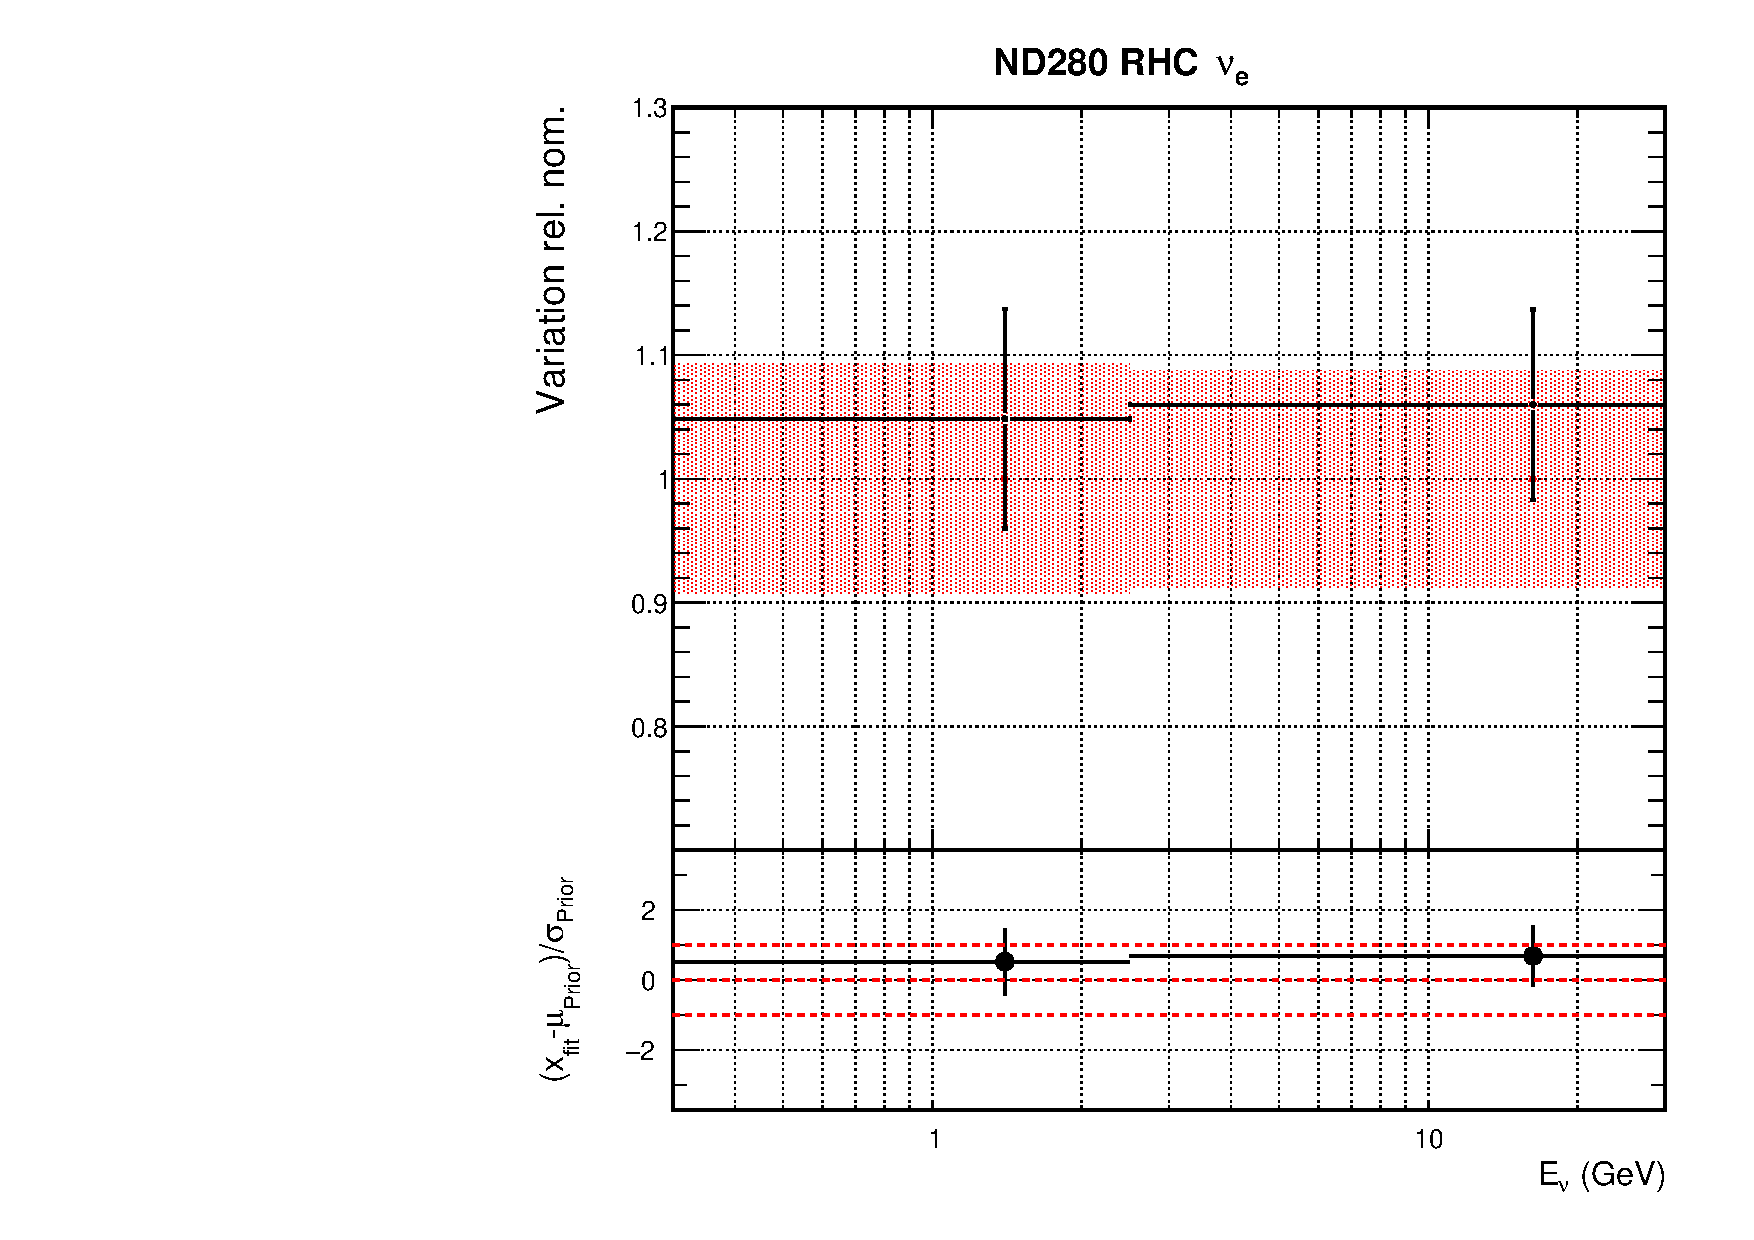
\includegraphics[width=0.75\linewidth]{figs/datflux6}
  \caption{ND RHC $\nu_{e}$}
\end{subfigure}
\begin{subfigure}{0.45\textwidth}
  \centering
  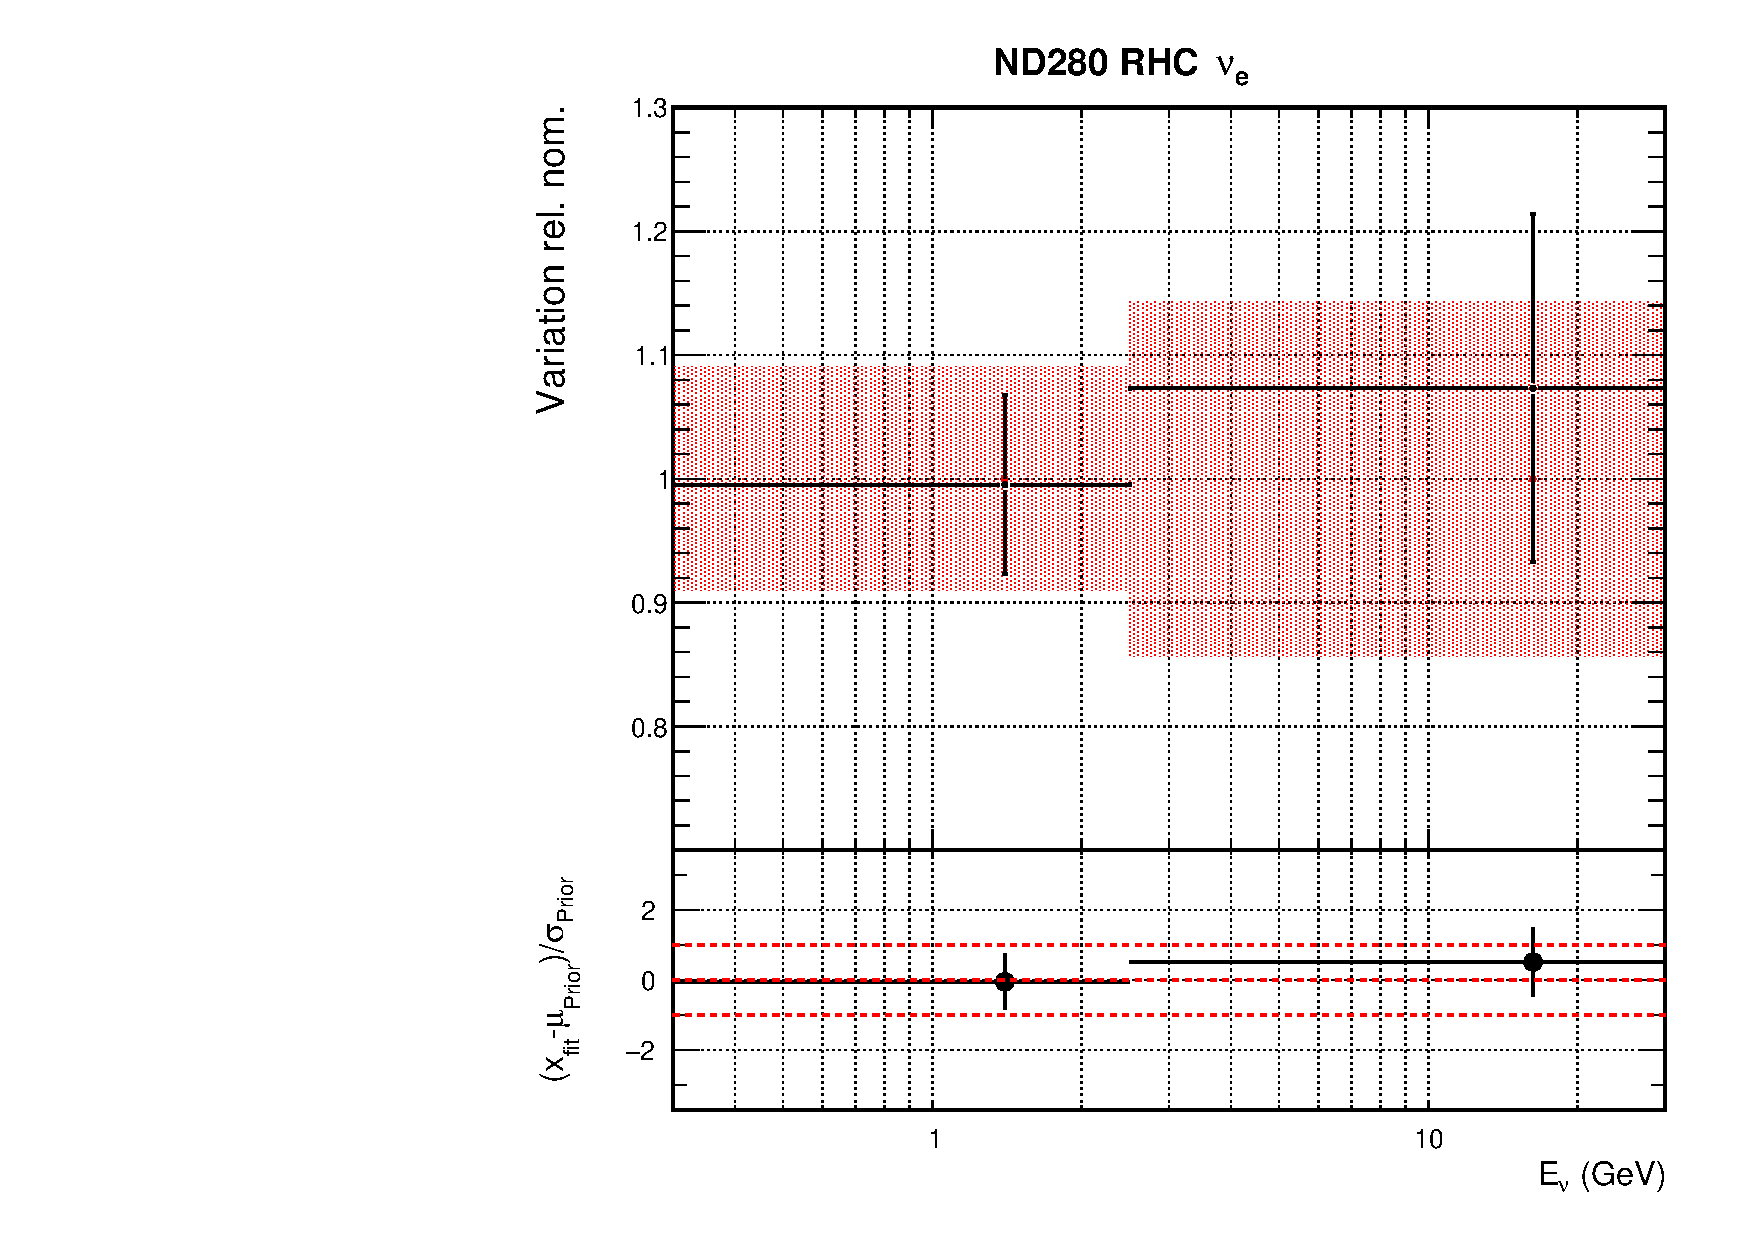
\includegraphics[width=0.75\linewidth]{figs/datflux7}
  \caption{ND RHC $\bar{\nu_e}$}
\end{subfigure}
\caption{ND280 flux parameters for the data fit.}
\label{fig:datfluxNDapp}
\end{figure}

\begin{figure}[!htbp]
\centering
\begin{subfigure}{0.8\textwidth}
  \centering
  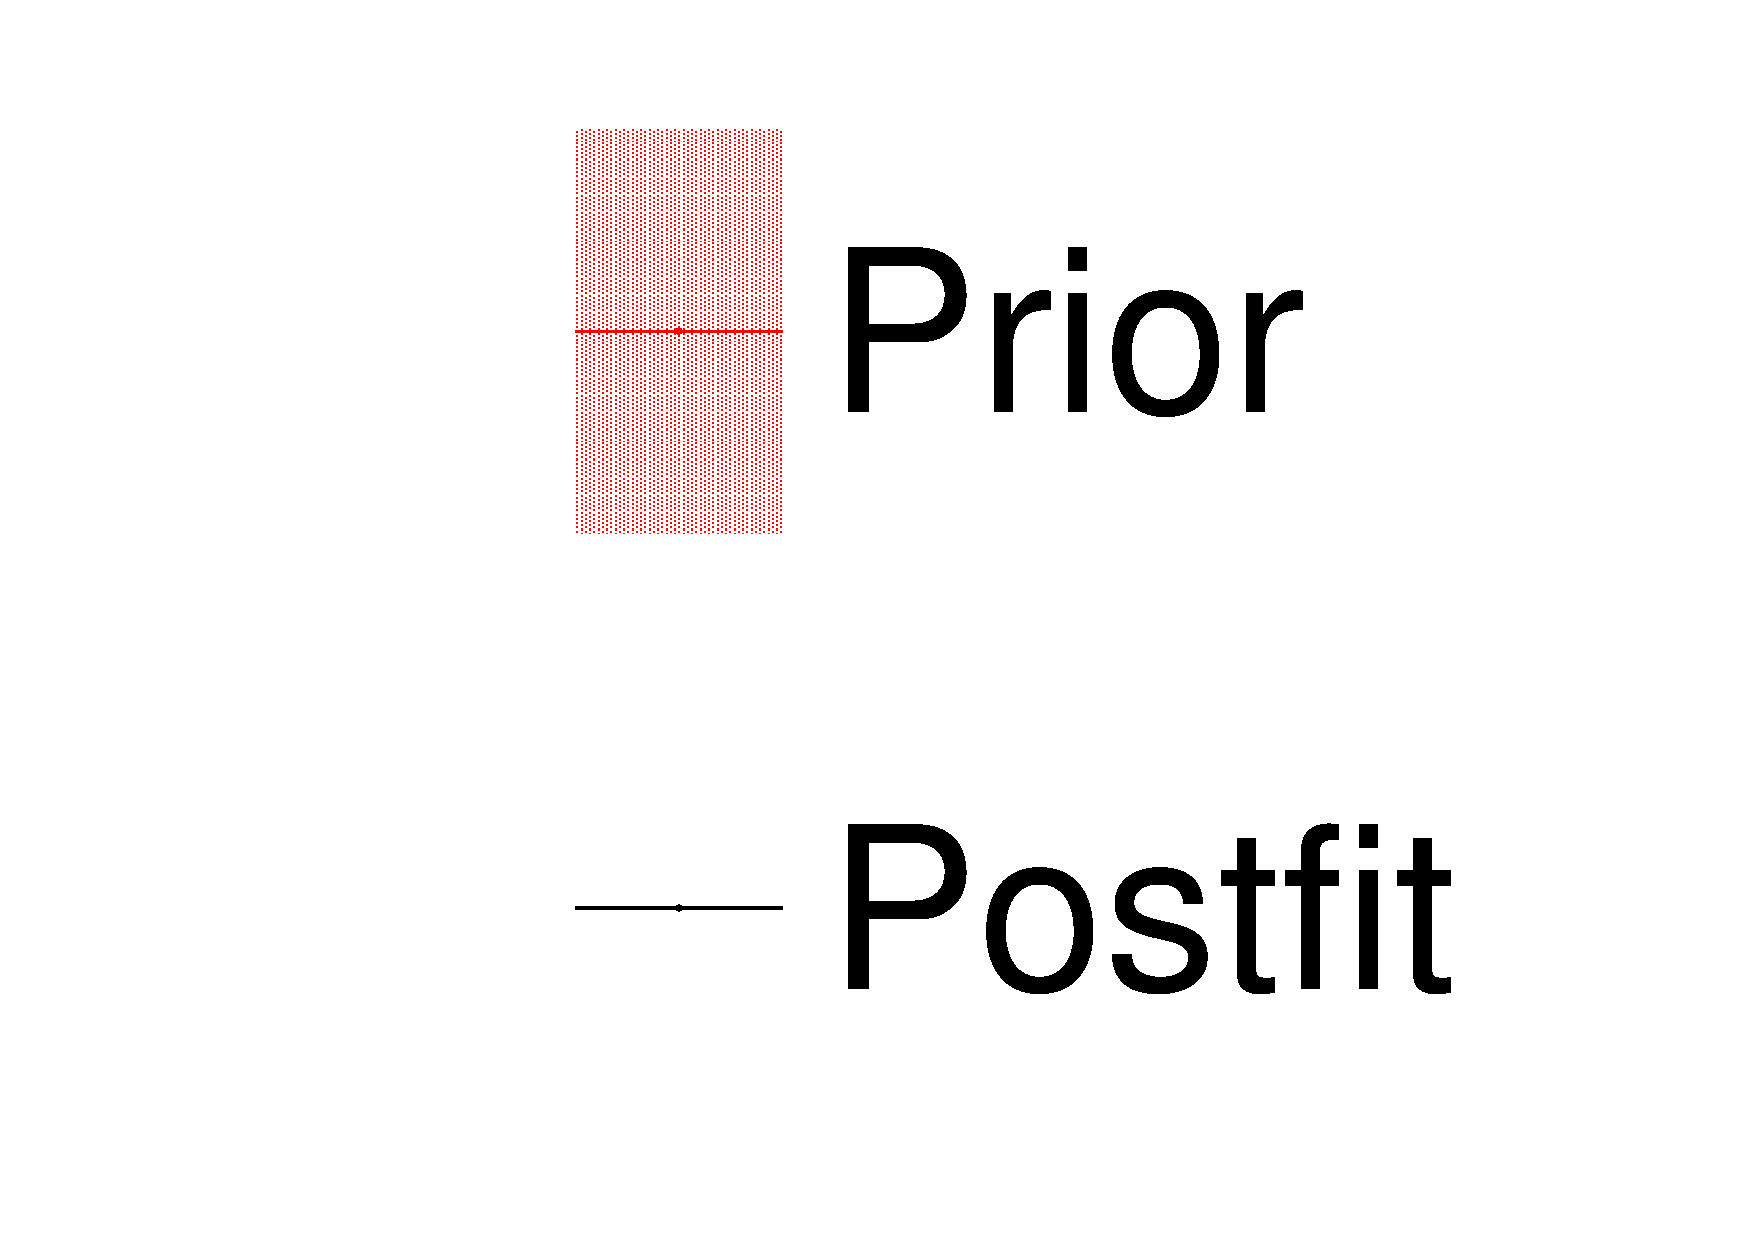
\includegraphics[width=0.24\linewidth]{figs/dat_leg}
\end{subfigure}
\begin{subfigure}{0.45\textwidth}
  \centering
  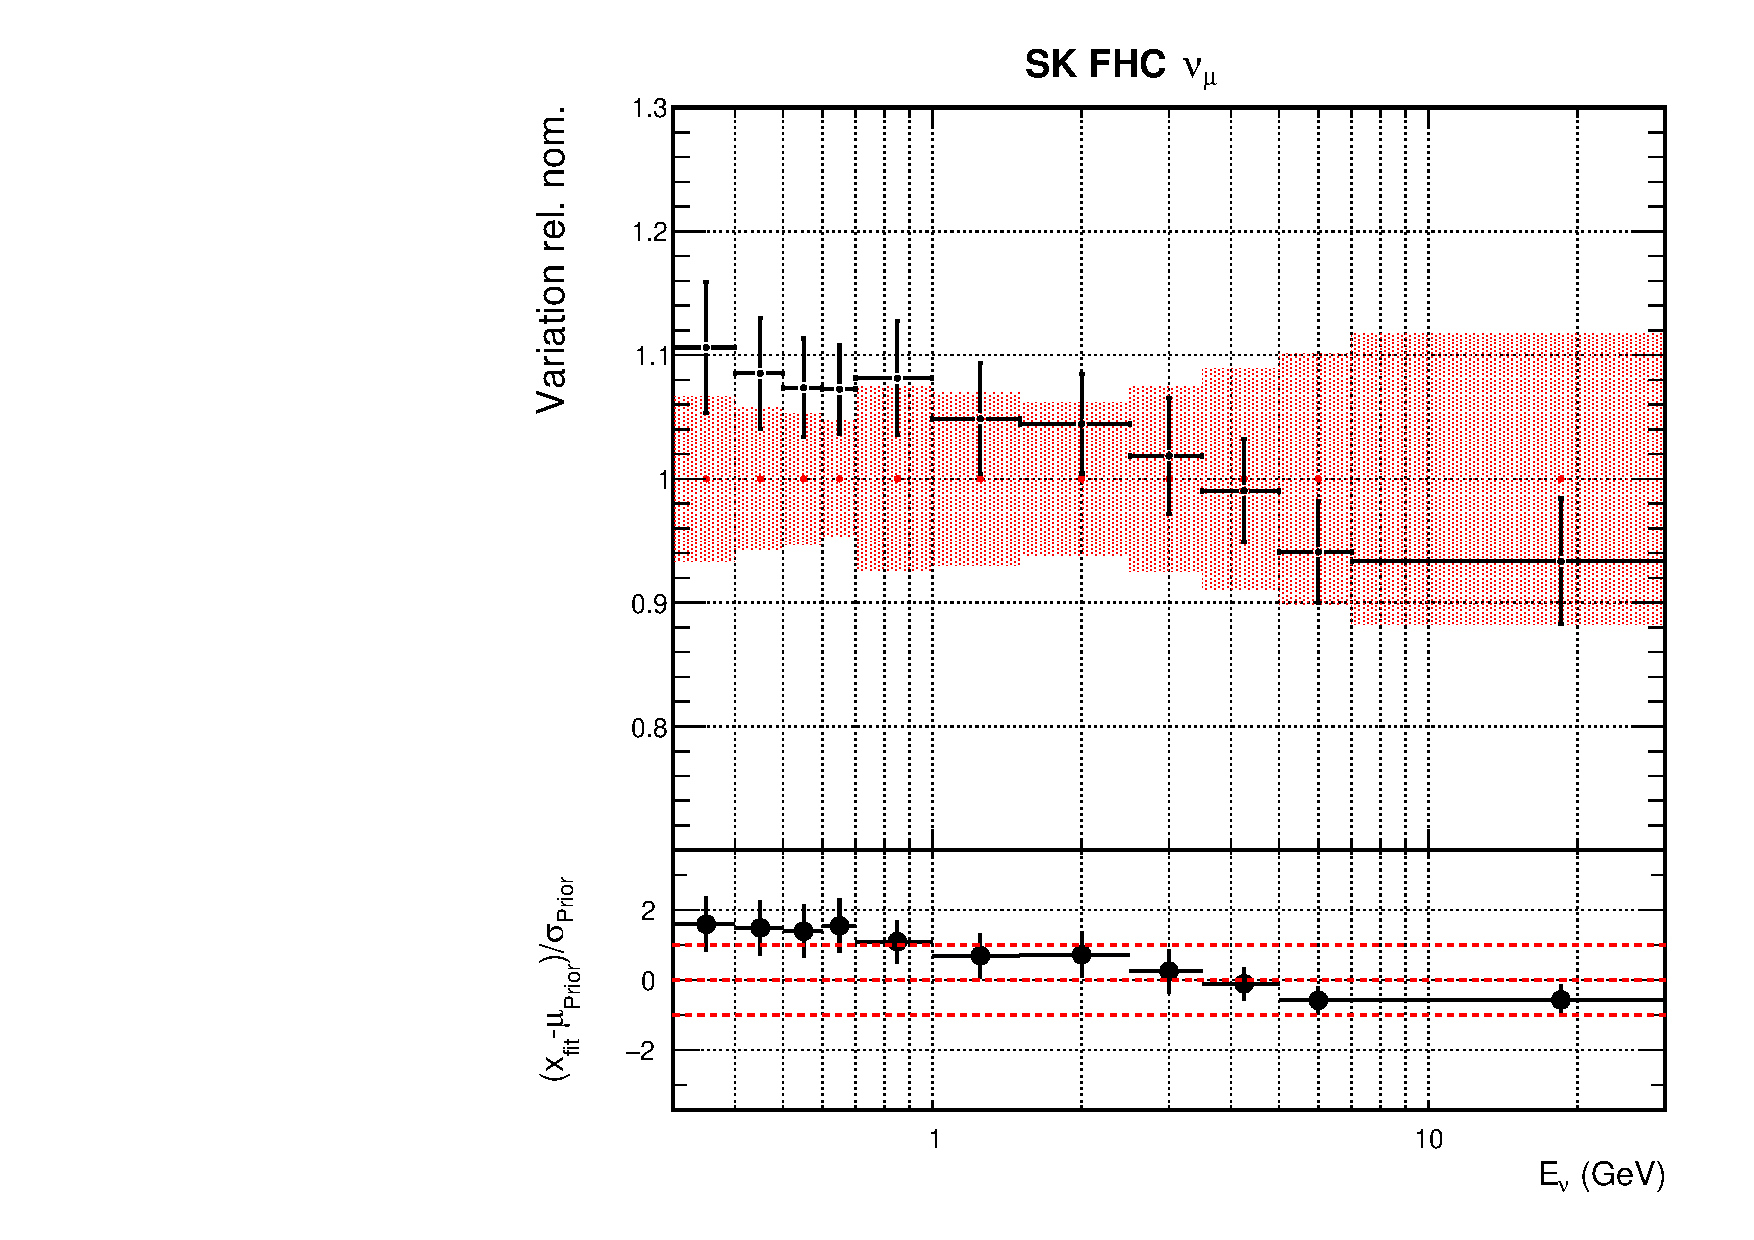
\includegraphics[width=0.75\linewidth]{figs/datflux8}
  \caption{\SK FHC $\nu_{\mu}$}
\end{subfigure}
\begin{subfigure}{0.45\textwidth}
  \centering
  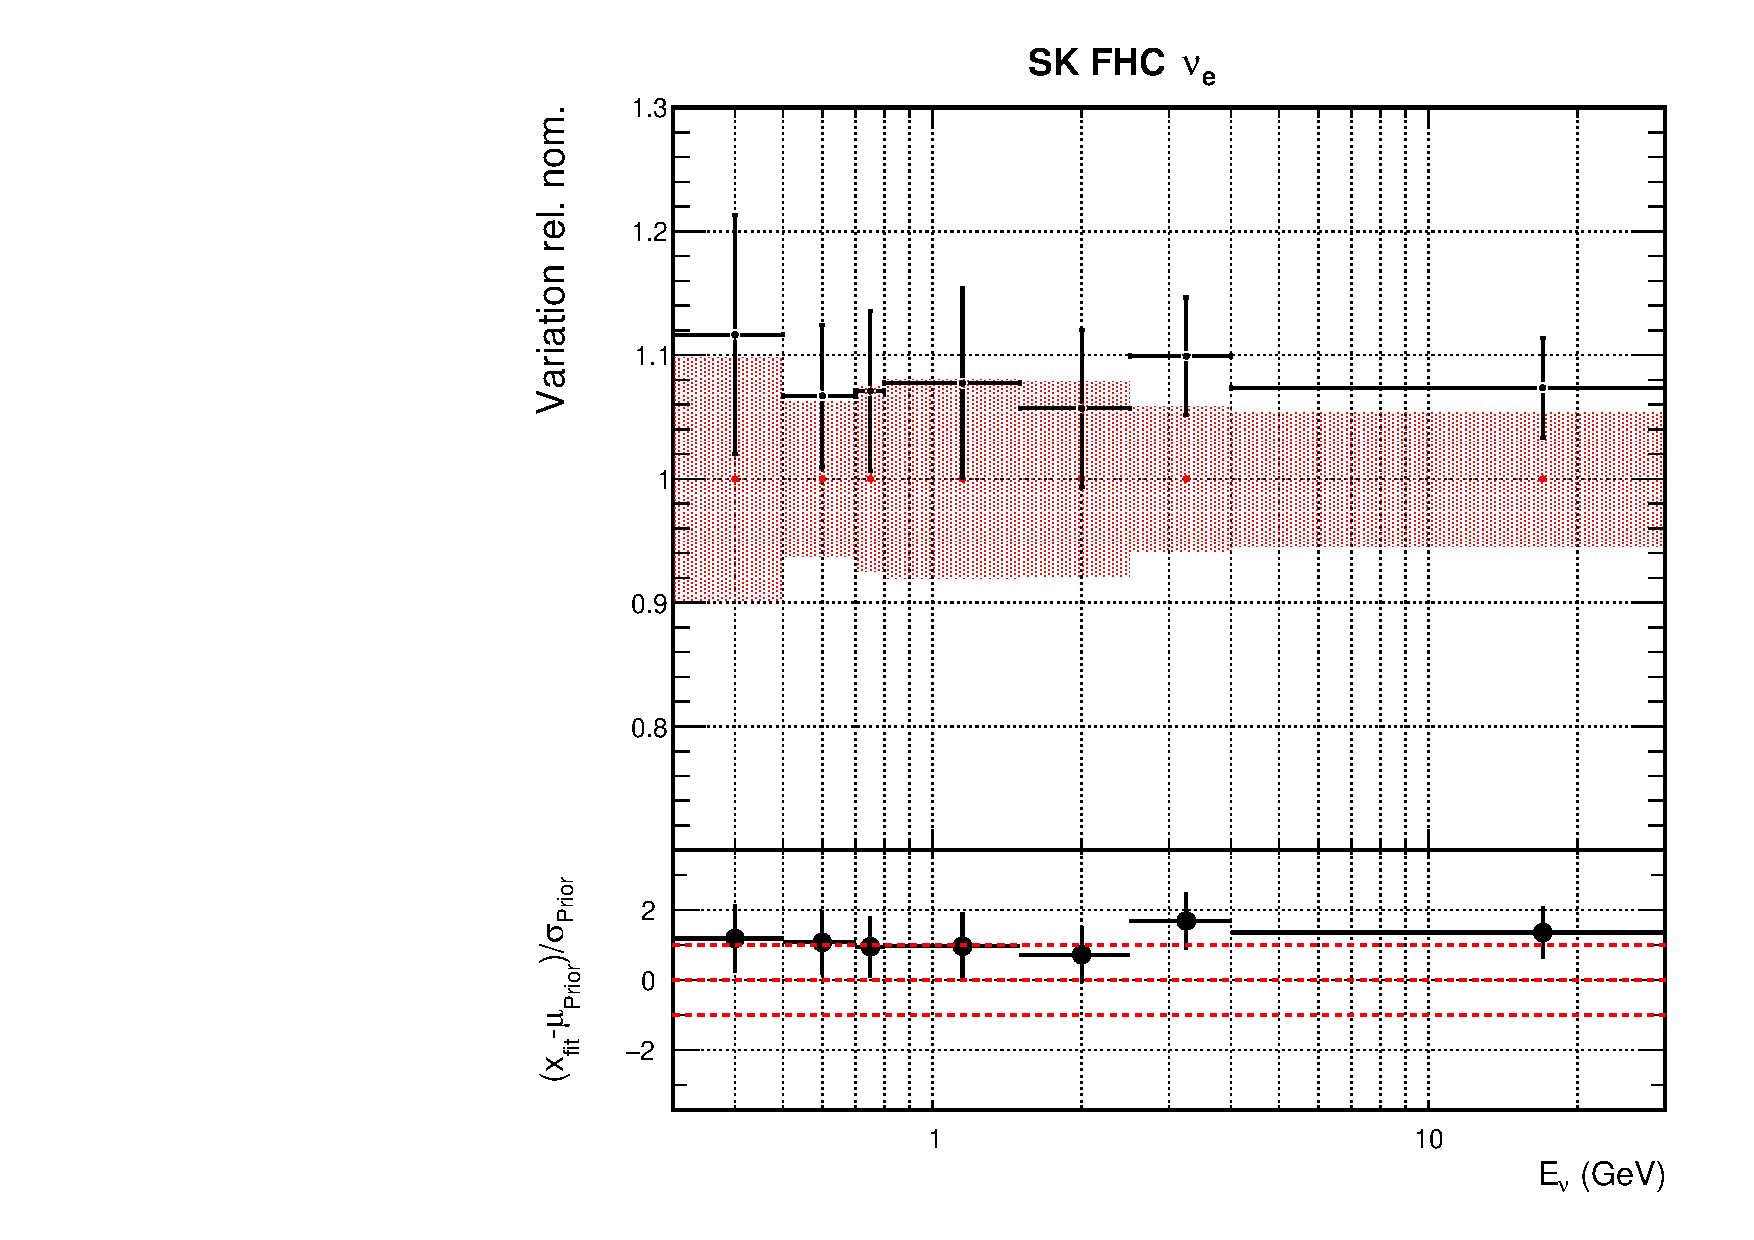
\includegraphics[width=0.75\linewidth]{figs/datflux9}
  \caption{\SK FHC $\bar{\nu_{\mu}}$}
\end{subfigure}
\begin{subfigure}{0.45\textwidth}
  \centering
  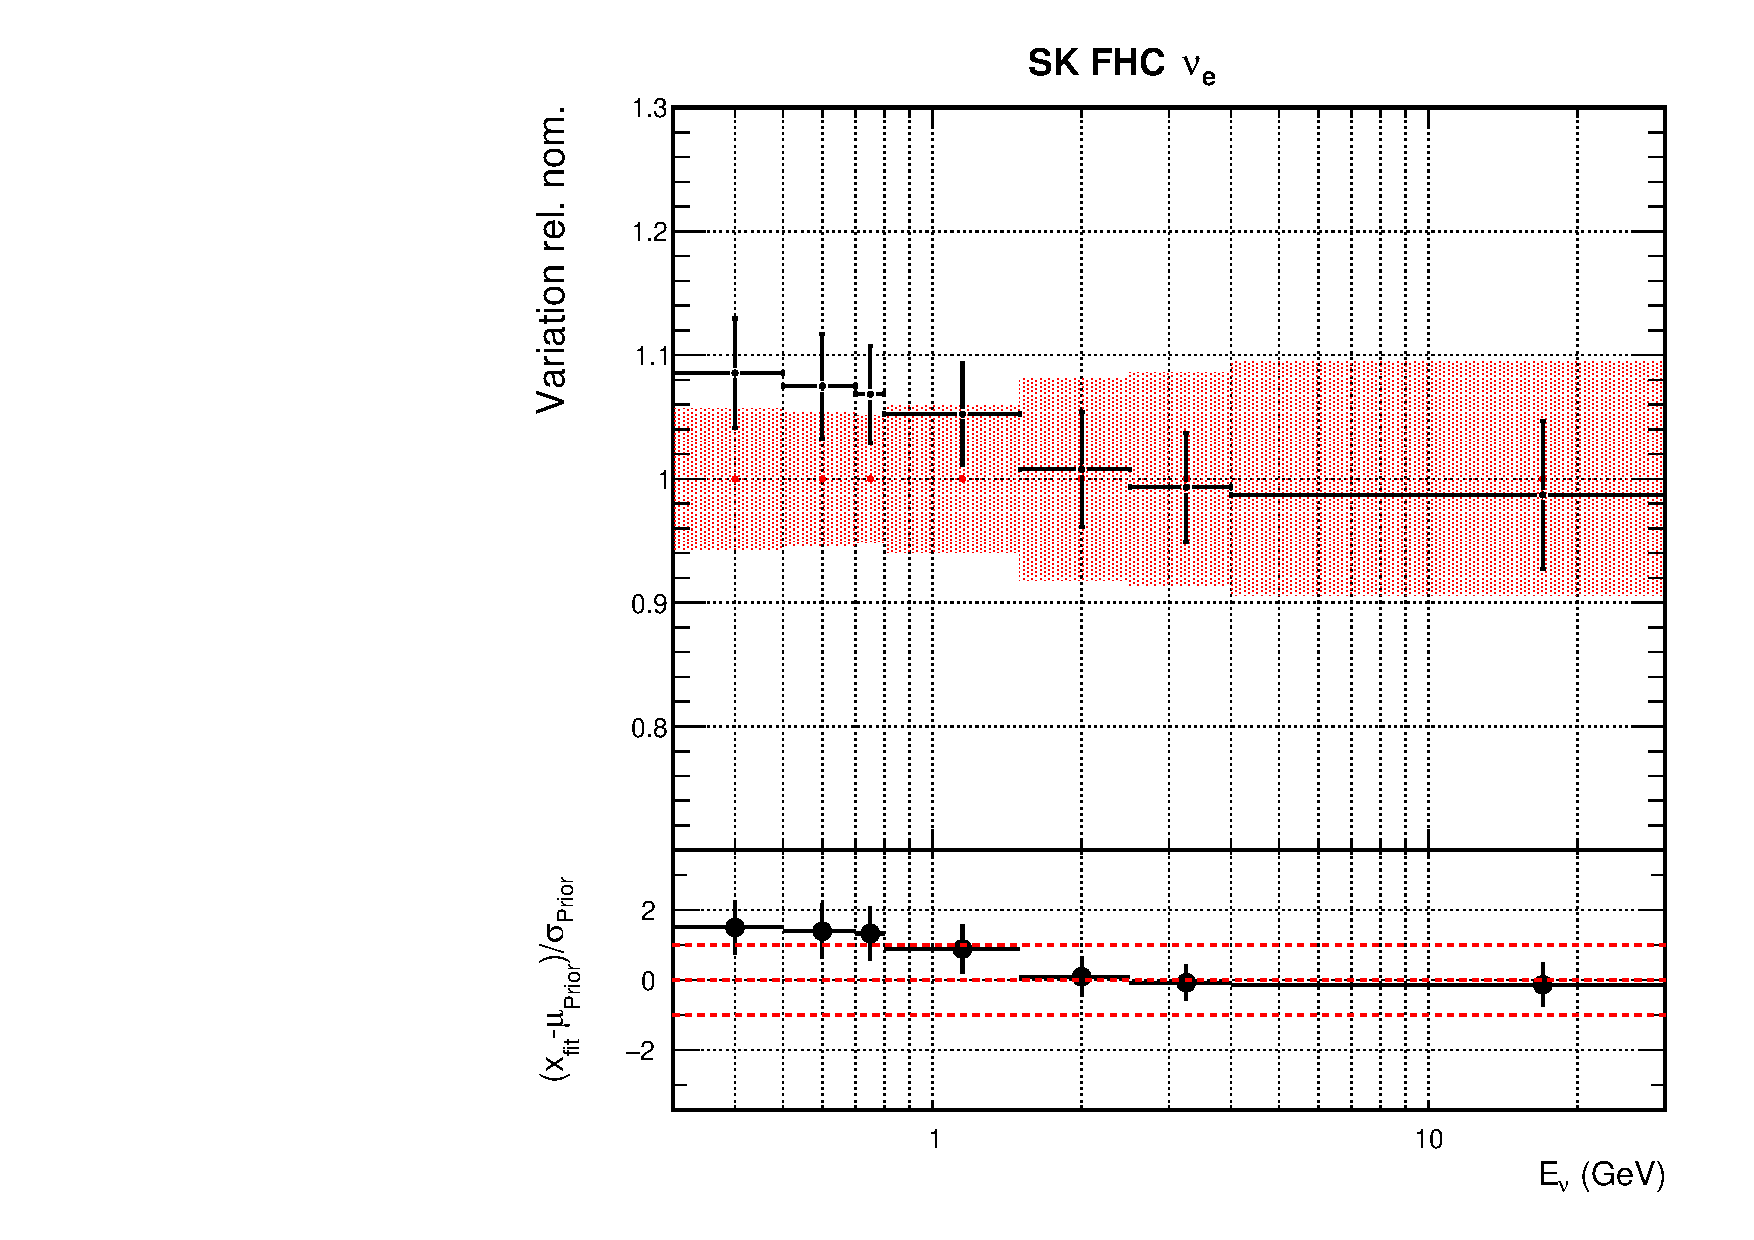
\includegraphics[width=0.75\linewidth]{figs/datflux10}
  \caption{\SK FHC $\nu_{e}$}
\end{subfigure}
\begin{subfigure}{0.45\textwidth}
  \centering
  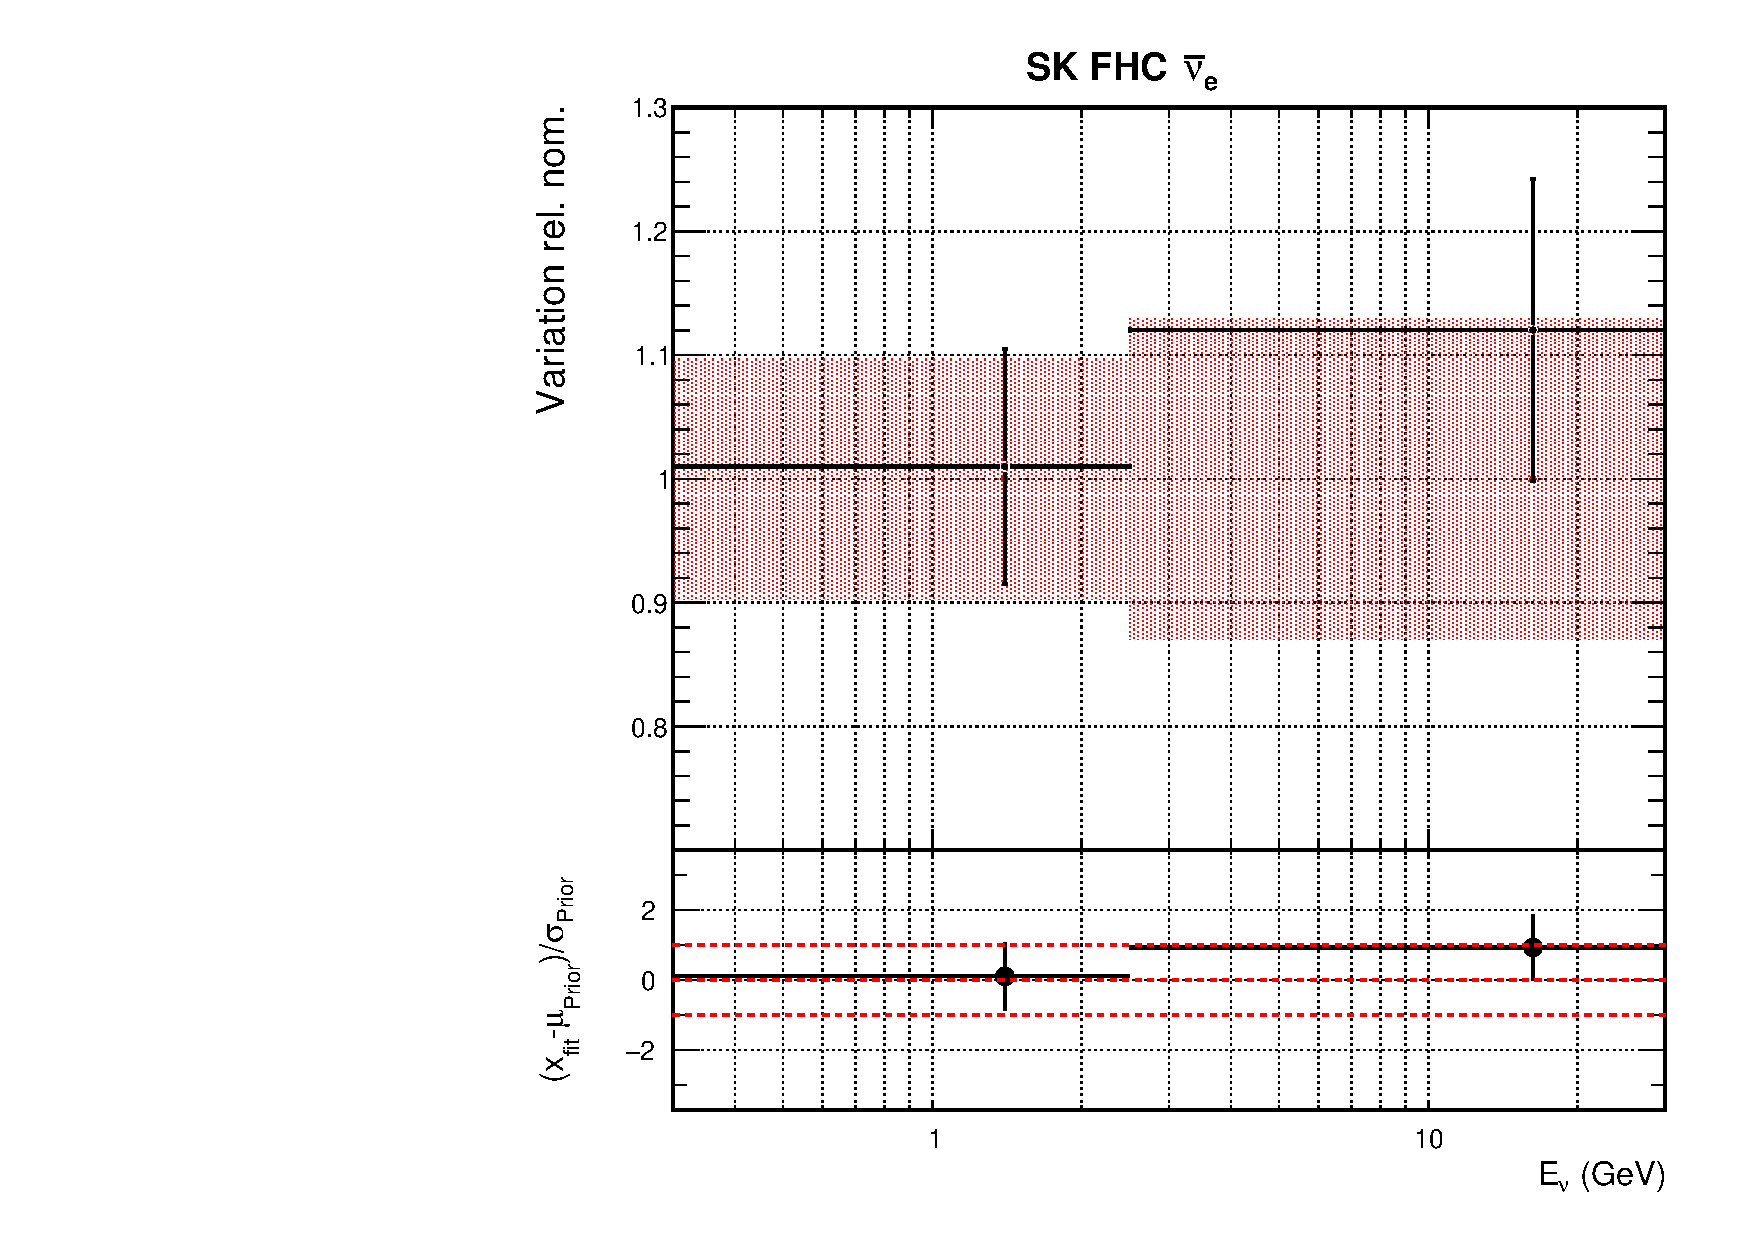
\includegraphics[width=0.75\linewidth]{figs/datflux11}
  \caption{\SK FHC $\bar{\nu_{e}}$}
\end{subfigure}
\begin{subfigure}{0.45\textwidth}
  \centering
  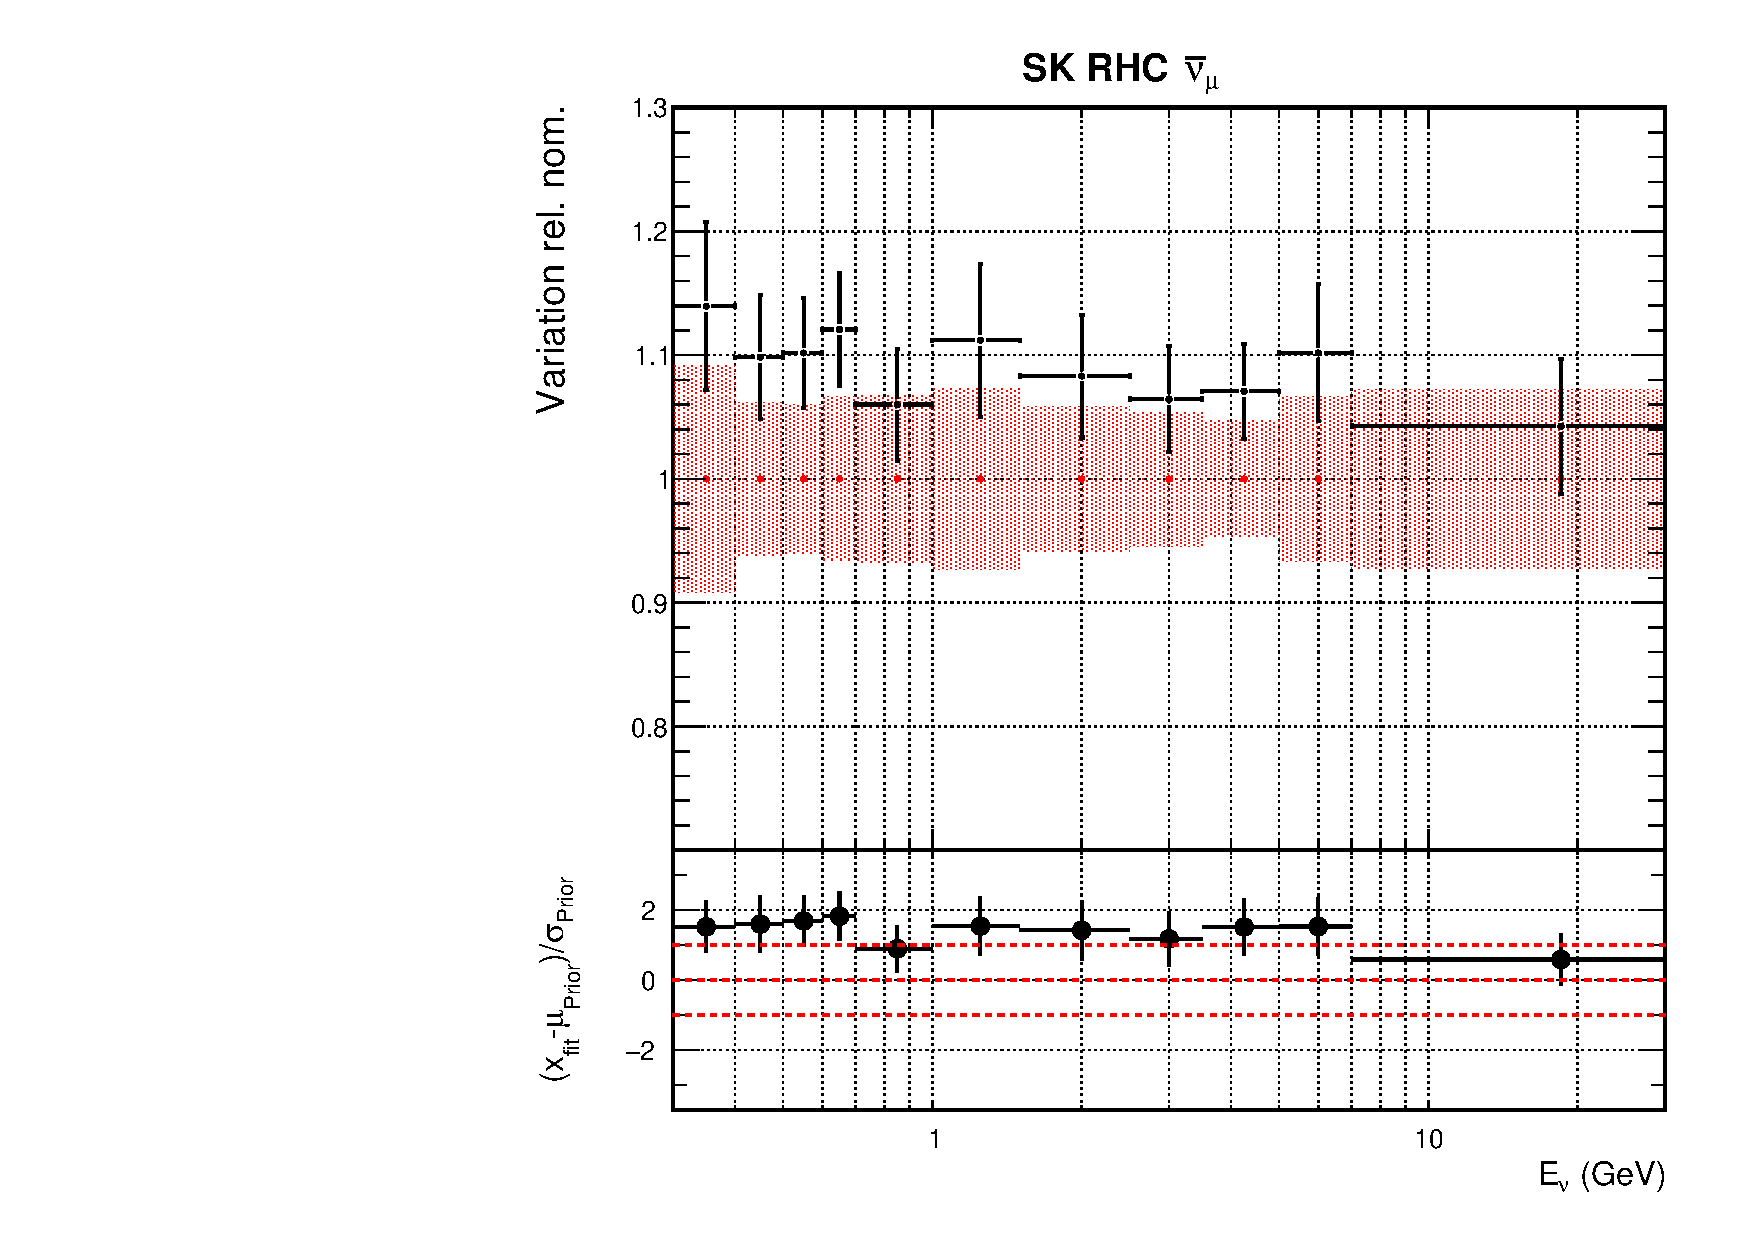
\includegraphics[width=0.75\linewidth]{figs/datflux12}
  \caption{\SK RHC $\nu_{\mu}$}
\end{subfigure}
\begin{subfigure}{0.45\textwidth}
  \centering
  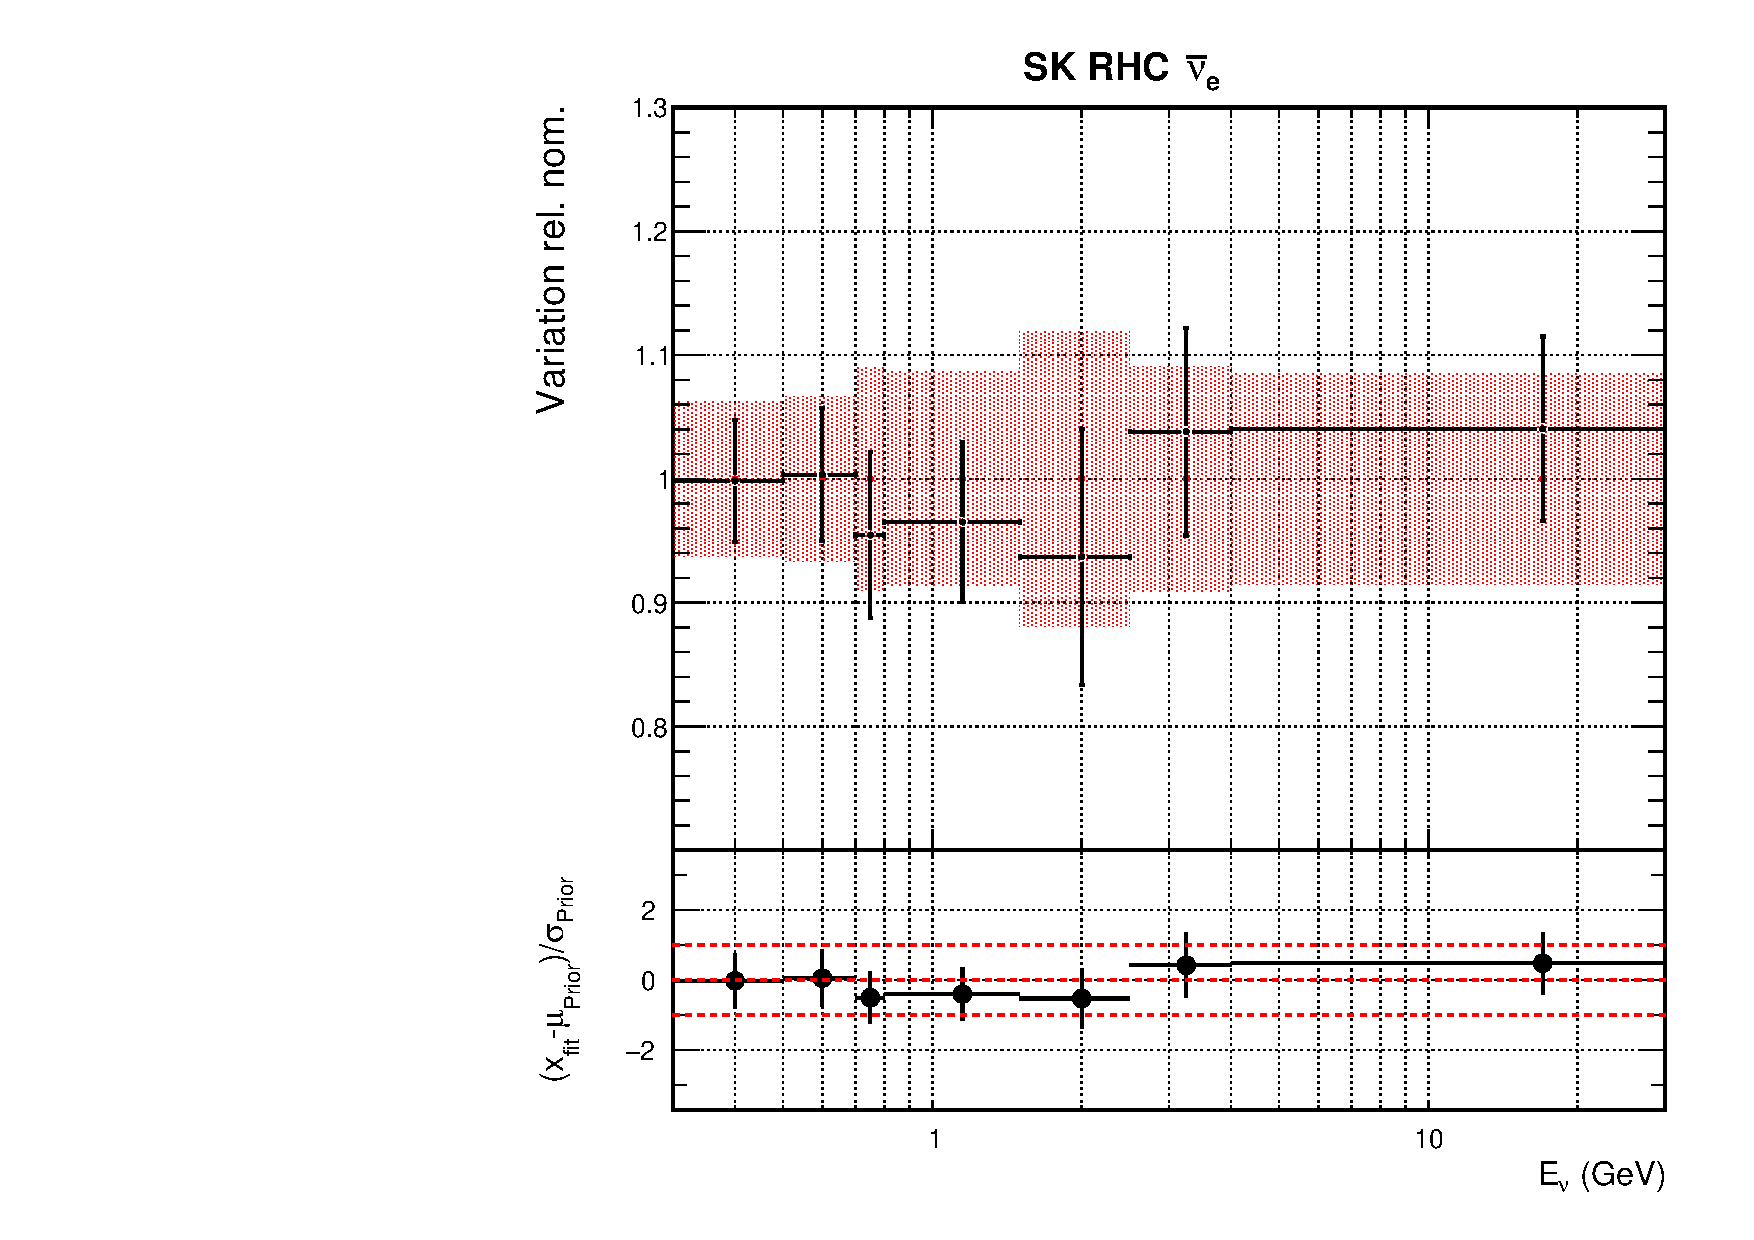
\includegraphics[width=0.75\linewidth]{figs/datflux13}
  \caption{\SK RHC $\bar{\nu_{\mu}}$}
\end{subfigure}
\begin{subfigure}{0.45\textwidth}
  \centering
  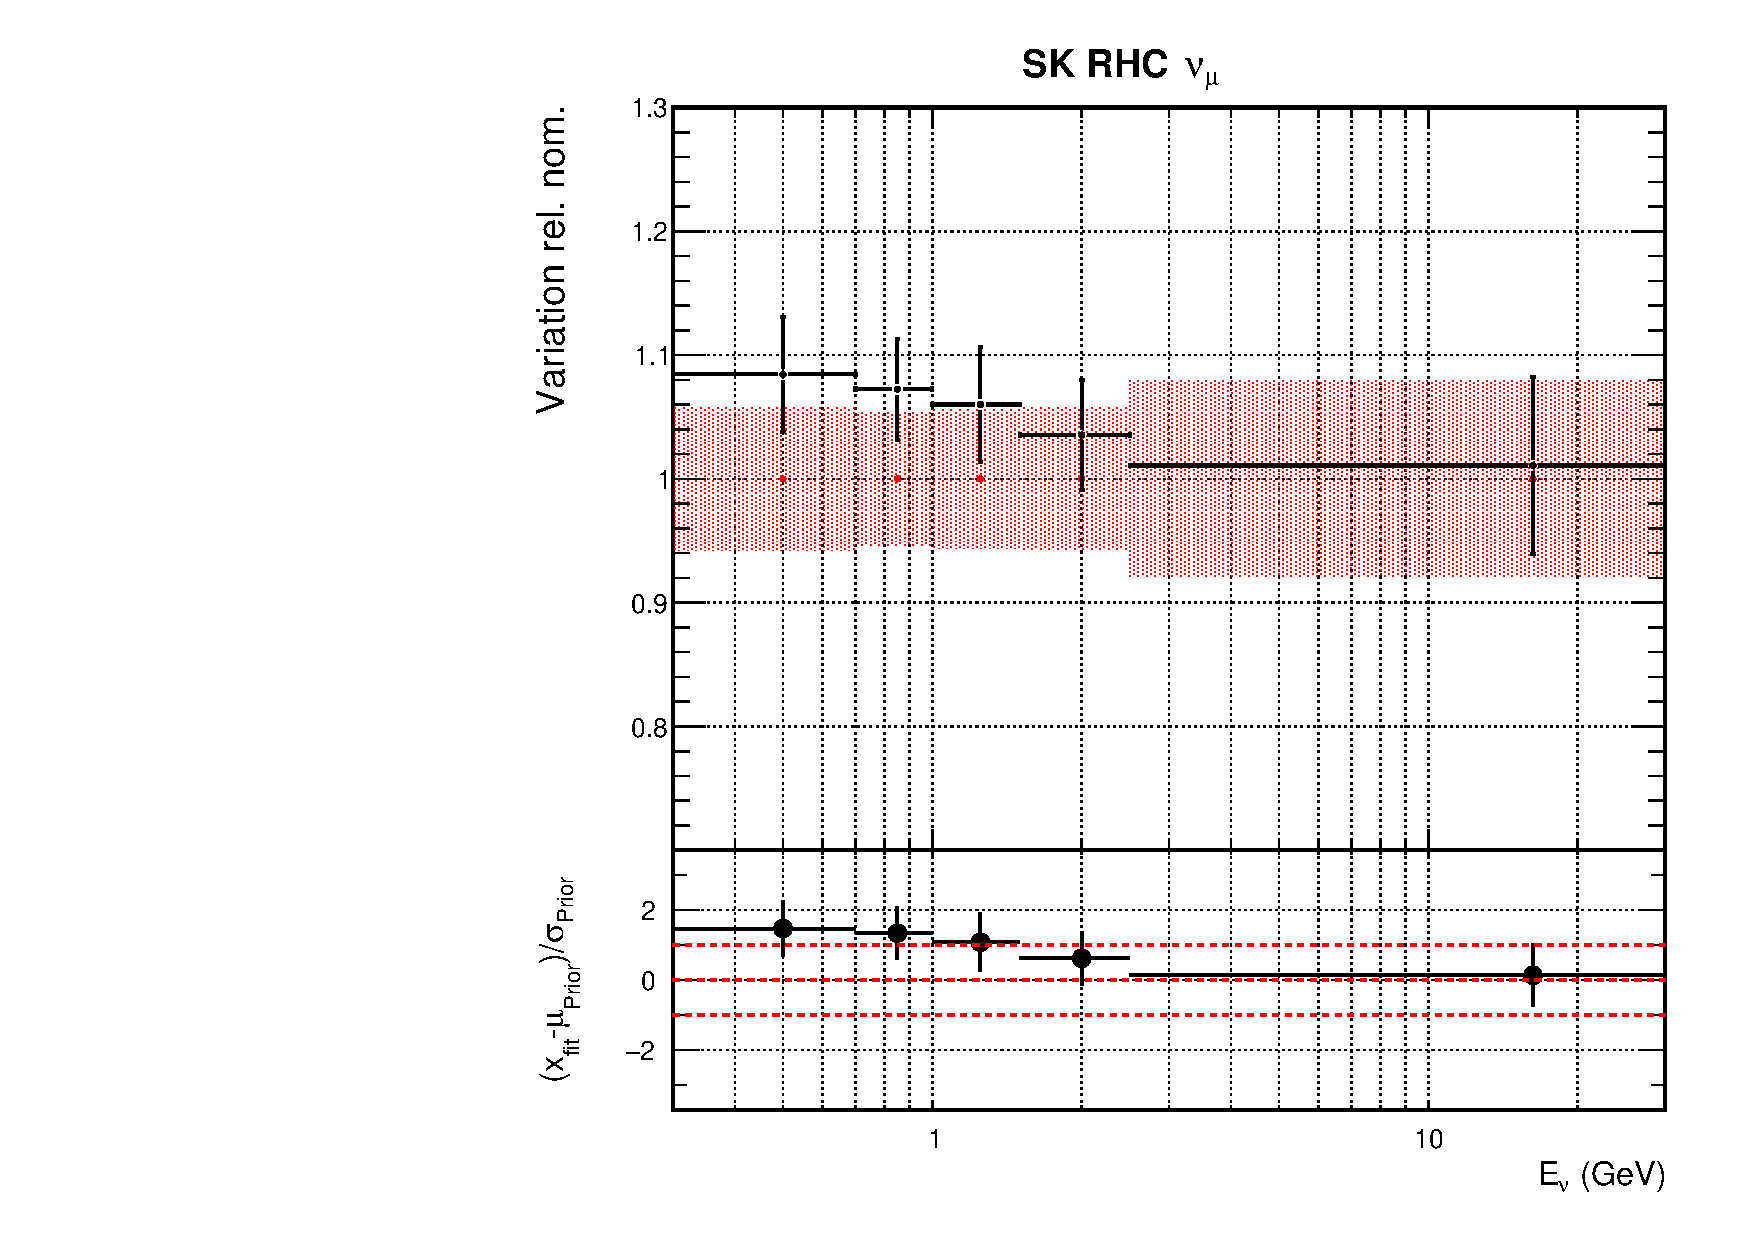
\includegraphics[width=0.75\linewidth]{figs/datflux14}
  \caption{\SK RHC $\nu_{e}$}
\end{subfigure}
\begin{subfigure}{0.45\textwidth}
  \centering
  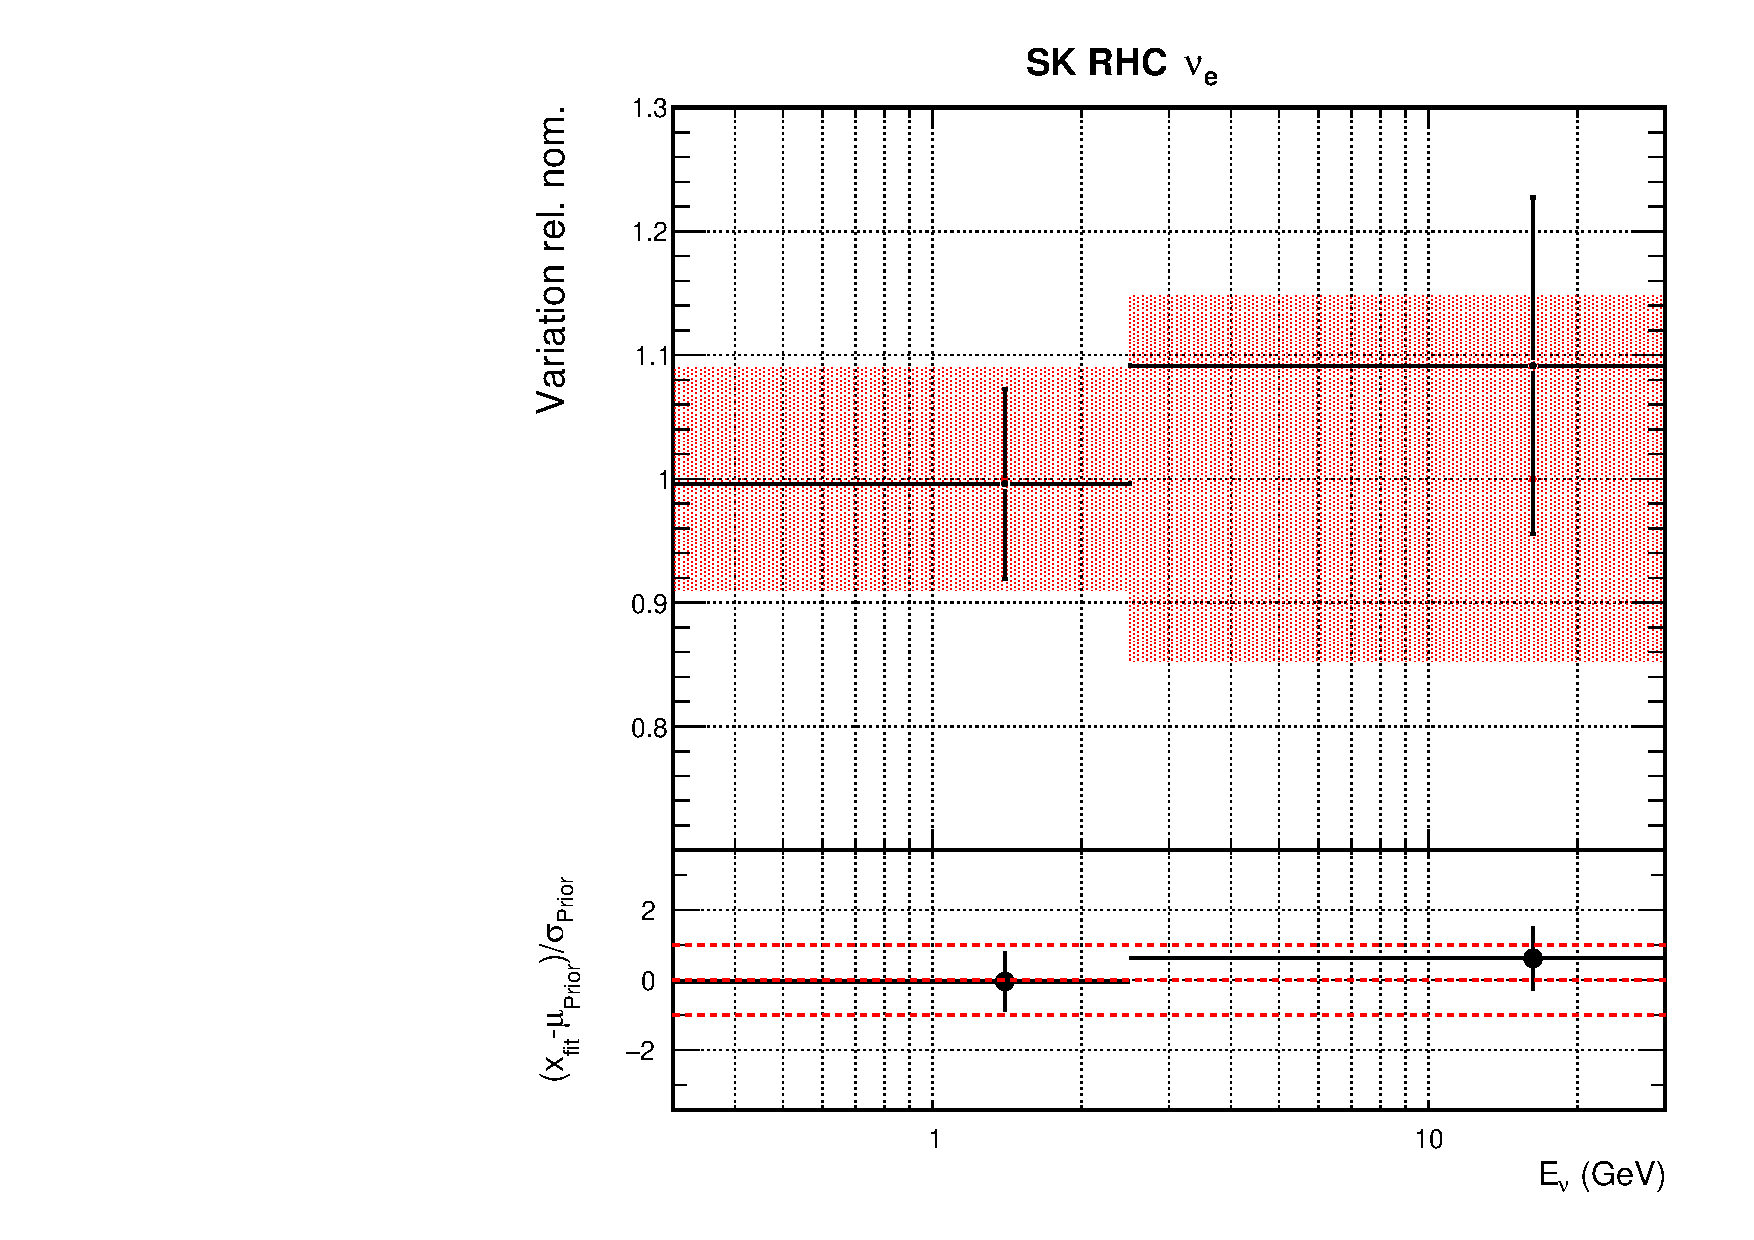
\includegraphics[width=0.75\linewidth]{figs/datflux15}
  \caption{\SK RHC $\bar{\nu_e}$}
\end{subfigure}
\caption{\SK flux parameters for the data fit.}
\label{fig:datfluxSKapp}
\end{figure}

\begin{figure}[!htbp]
\centering
\begin{subfigure}{0.95\textwidth}
  \centering
  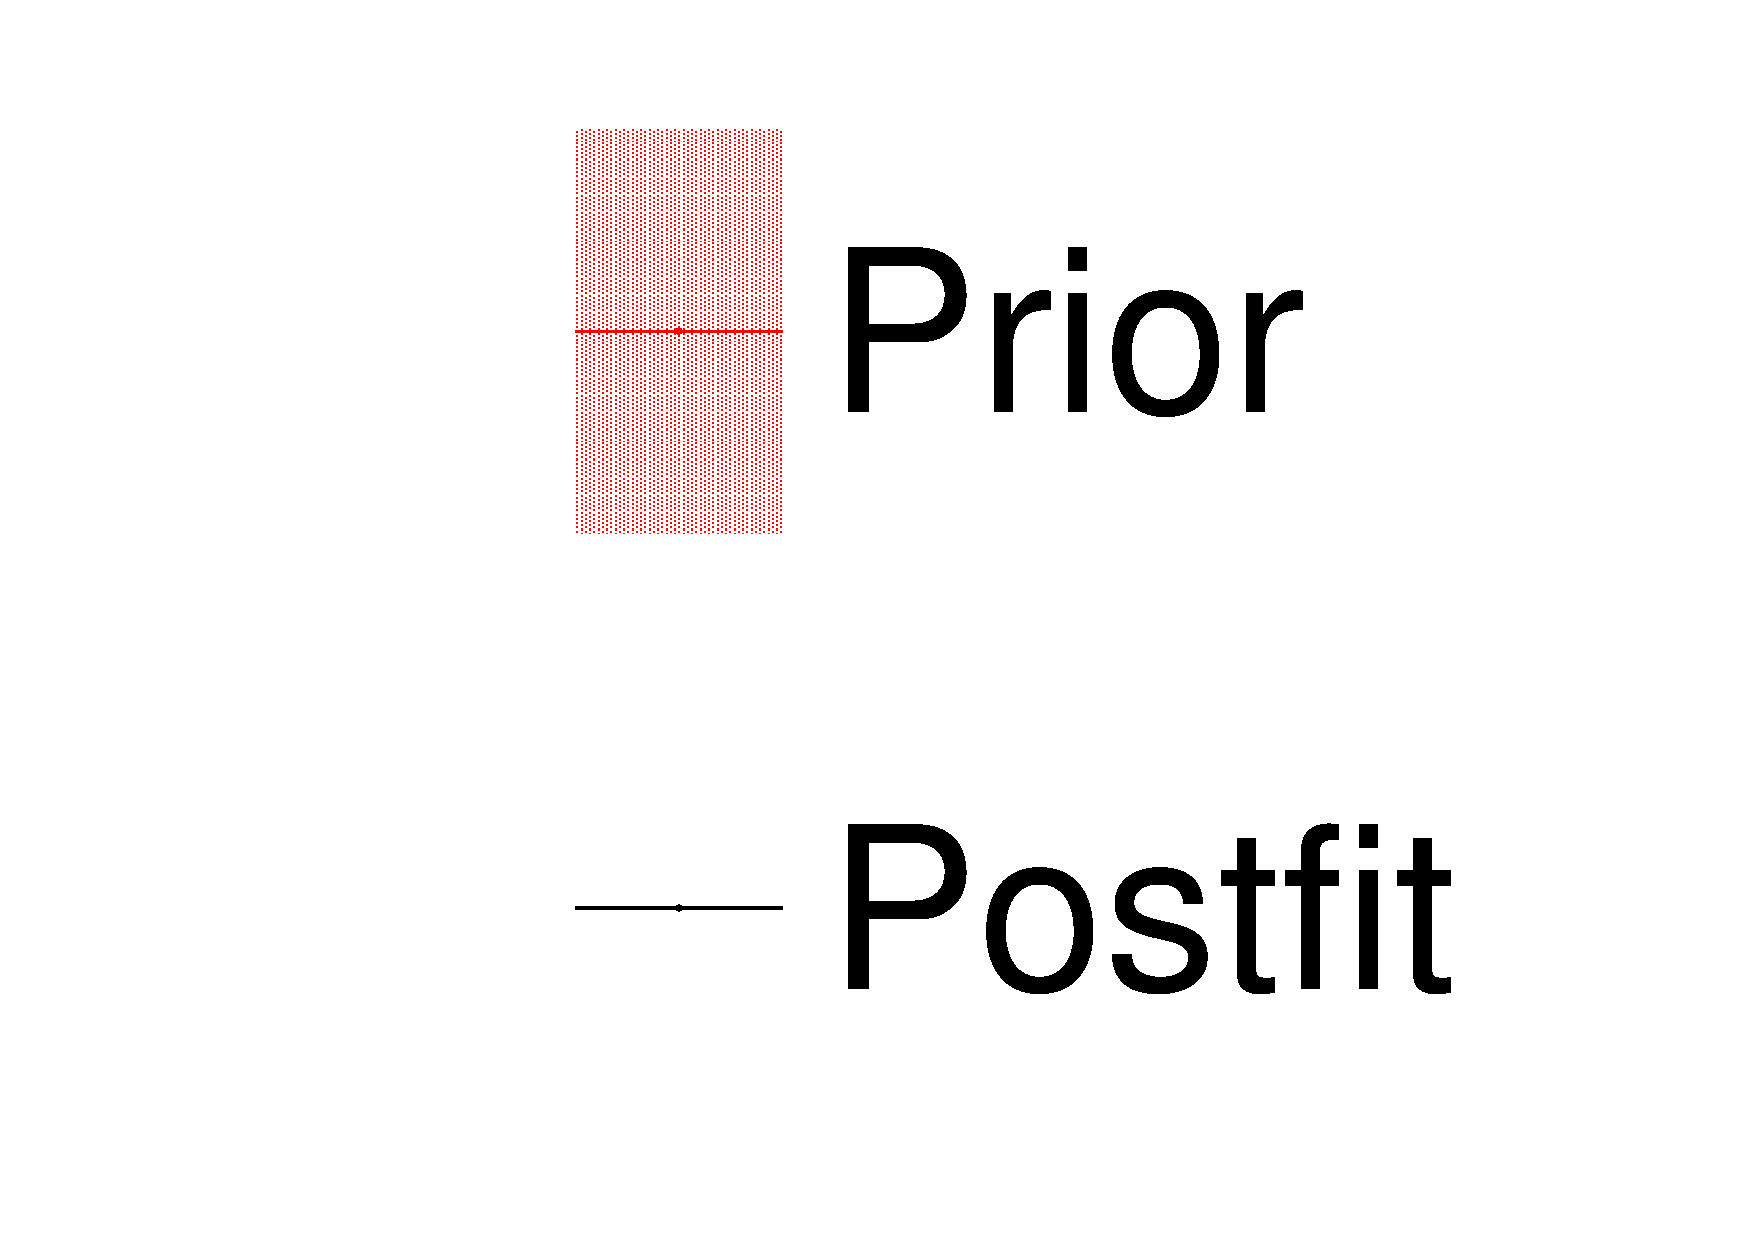
\includegraphics[width=0.25\linewidth]{figs/dat_leg}
\end{subfigure}
\begin{subfigure}{0.49\textwidth}
  \centering
  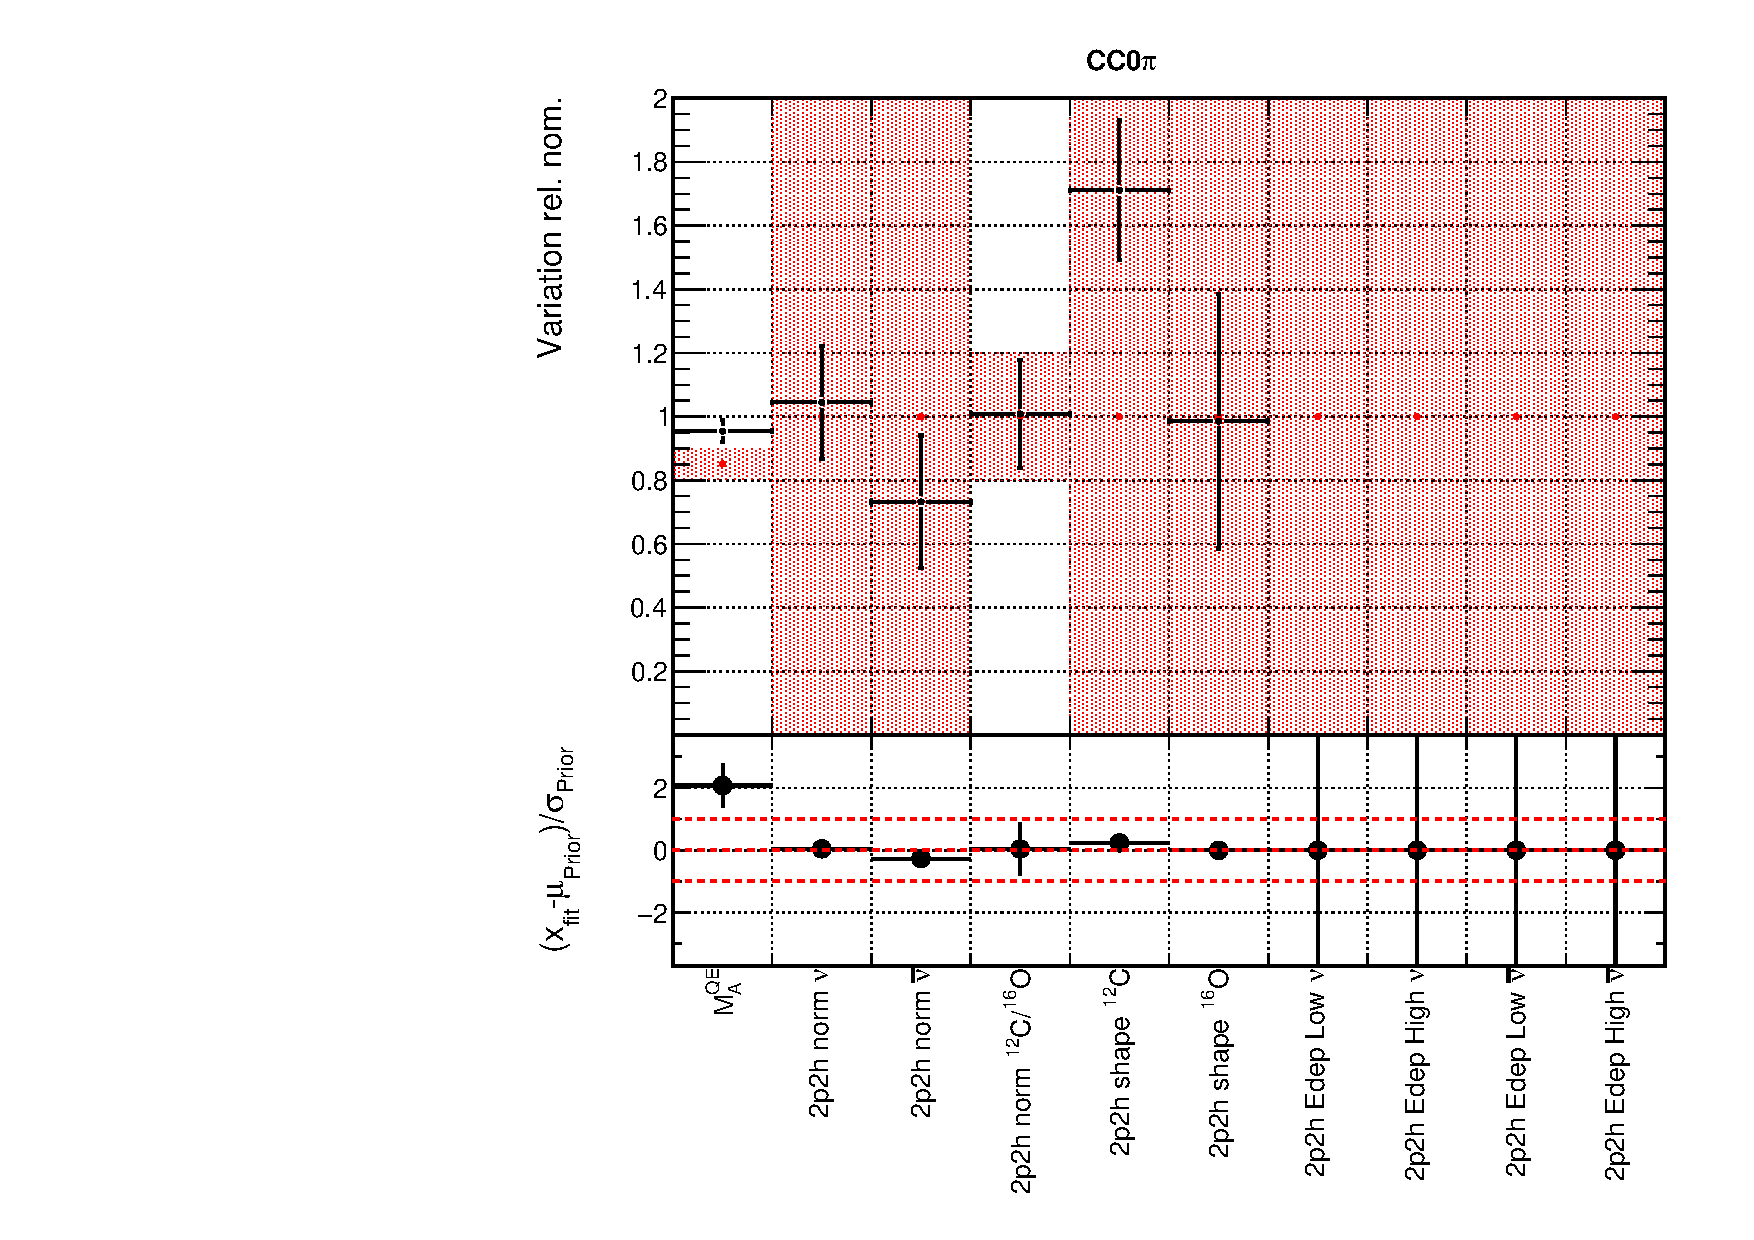
\includegraphics[width=0.9\linewidth]{figs/datxsec1}
  \caption{CC 0$\pi$}
\end{subfigure}
\begin{subfigure}{0.49\textwidth}
  \centering
  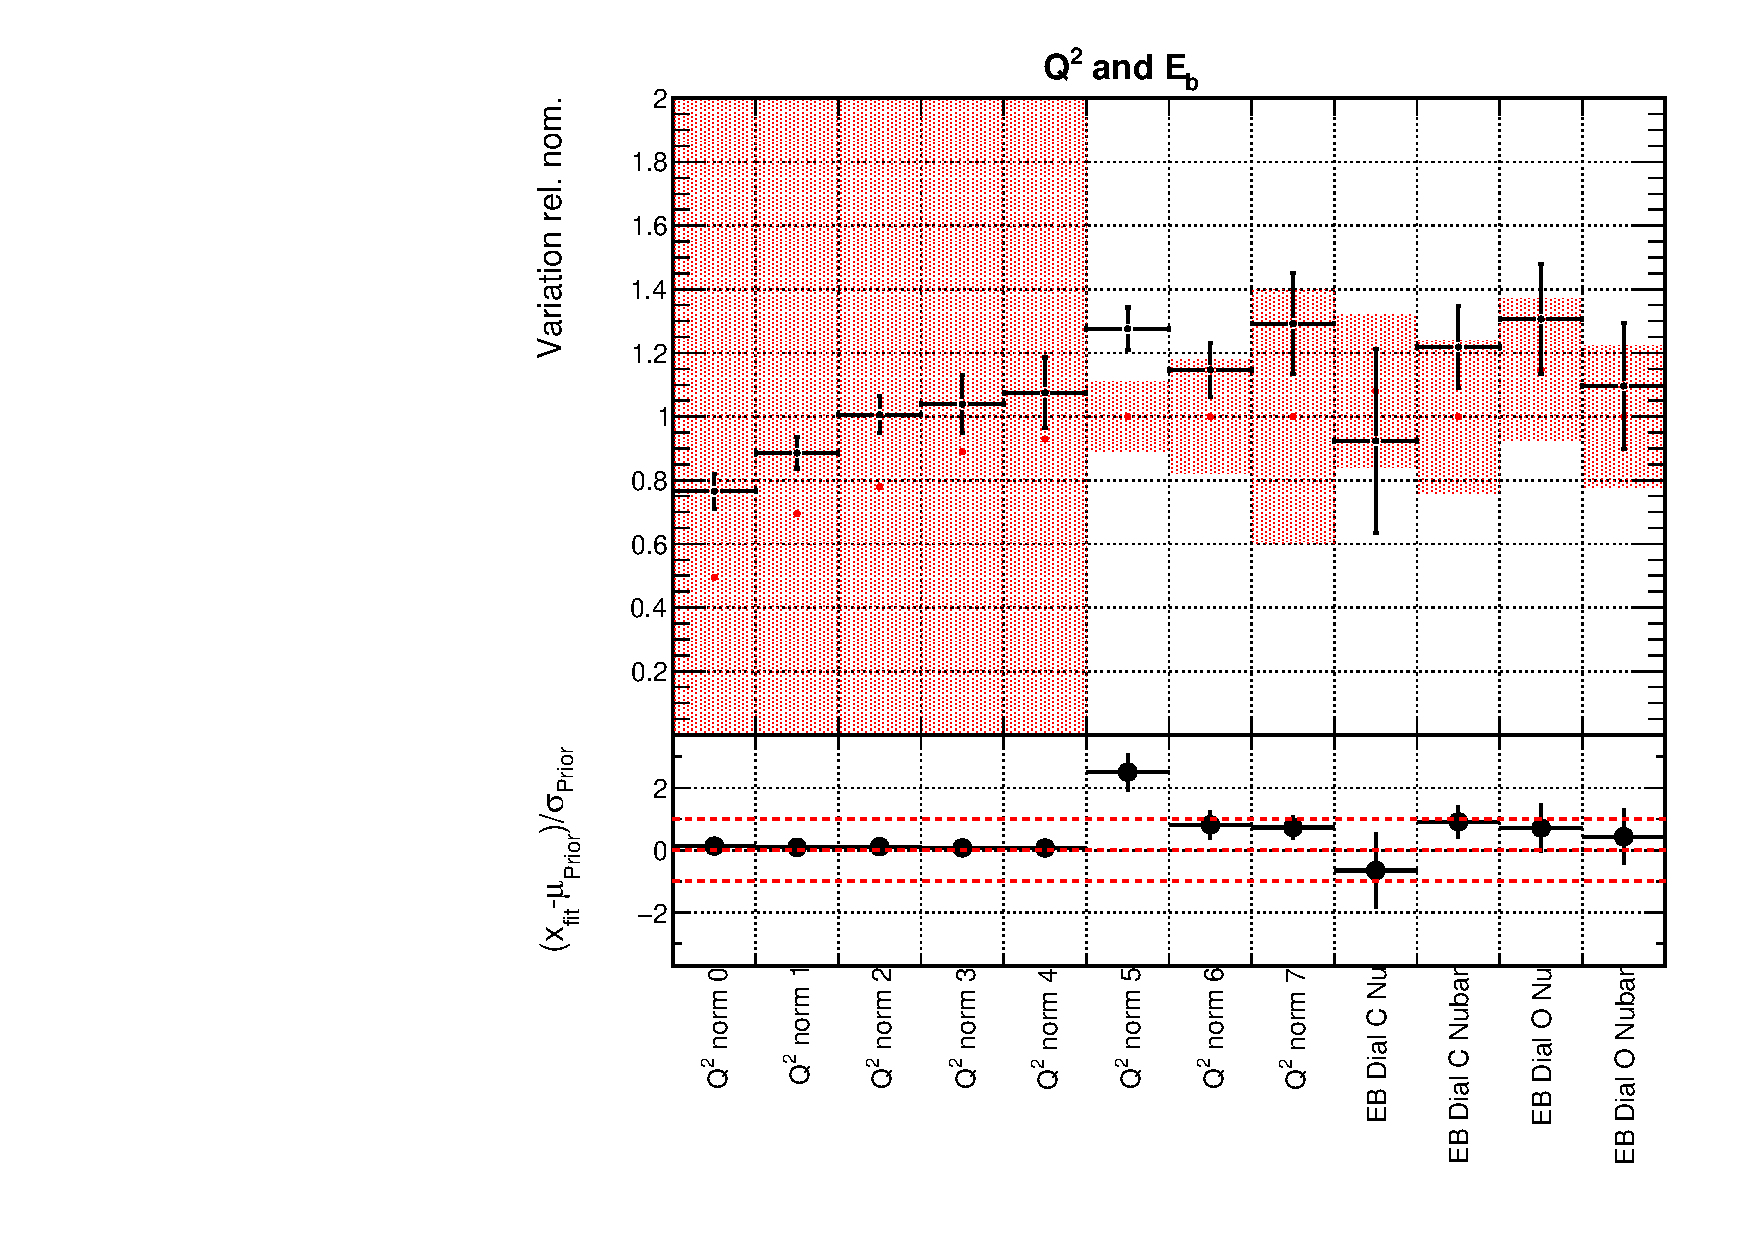
\includegraphics[width=0.9\linewidth]{figs/datxsec2}
  \caption{$Q^2$ and $E_{\mathrm{b}}$}
\end{subfigure}
\begin{subfigure}{0.49\textwidth}
  \centering
  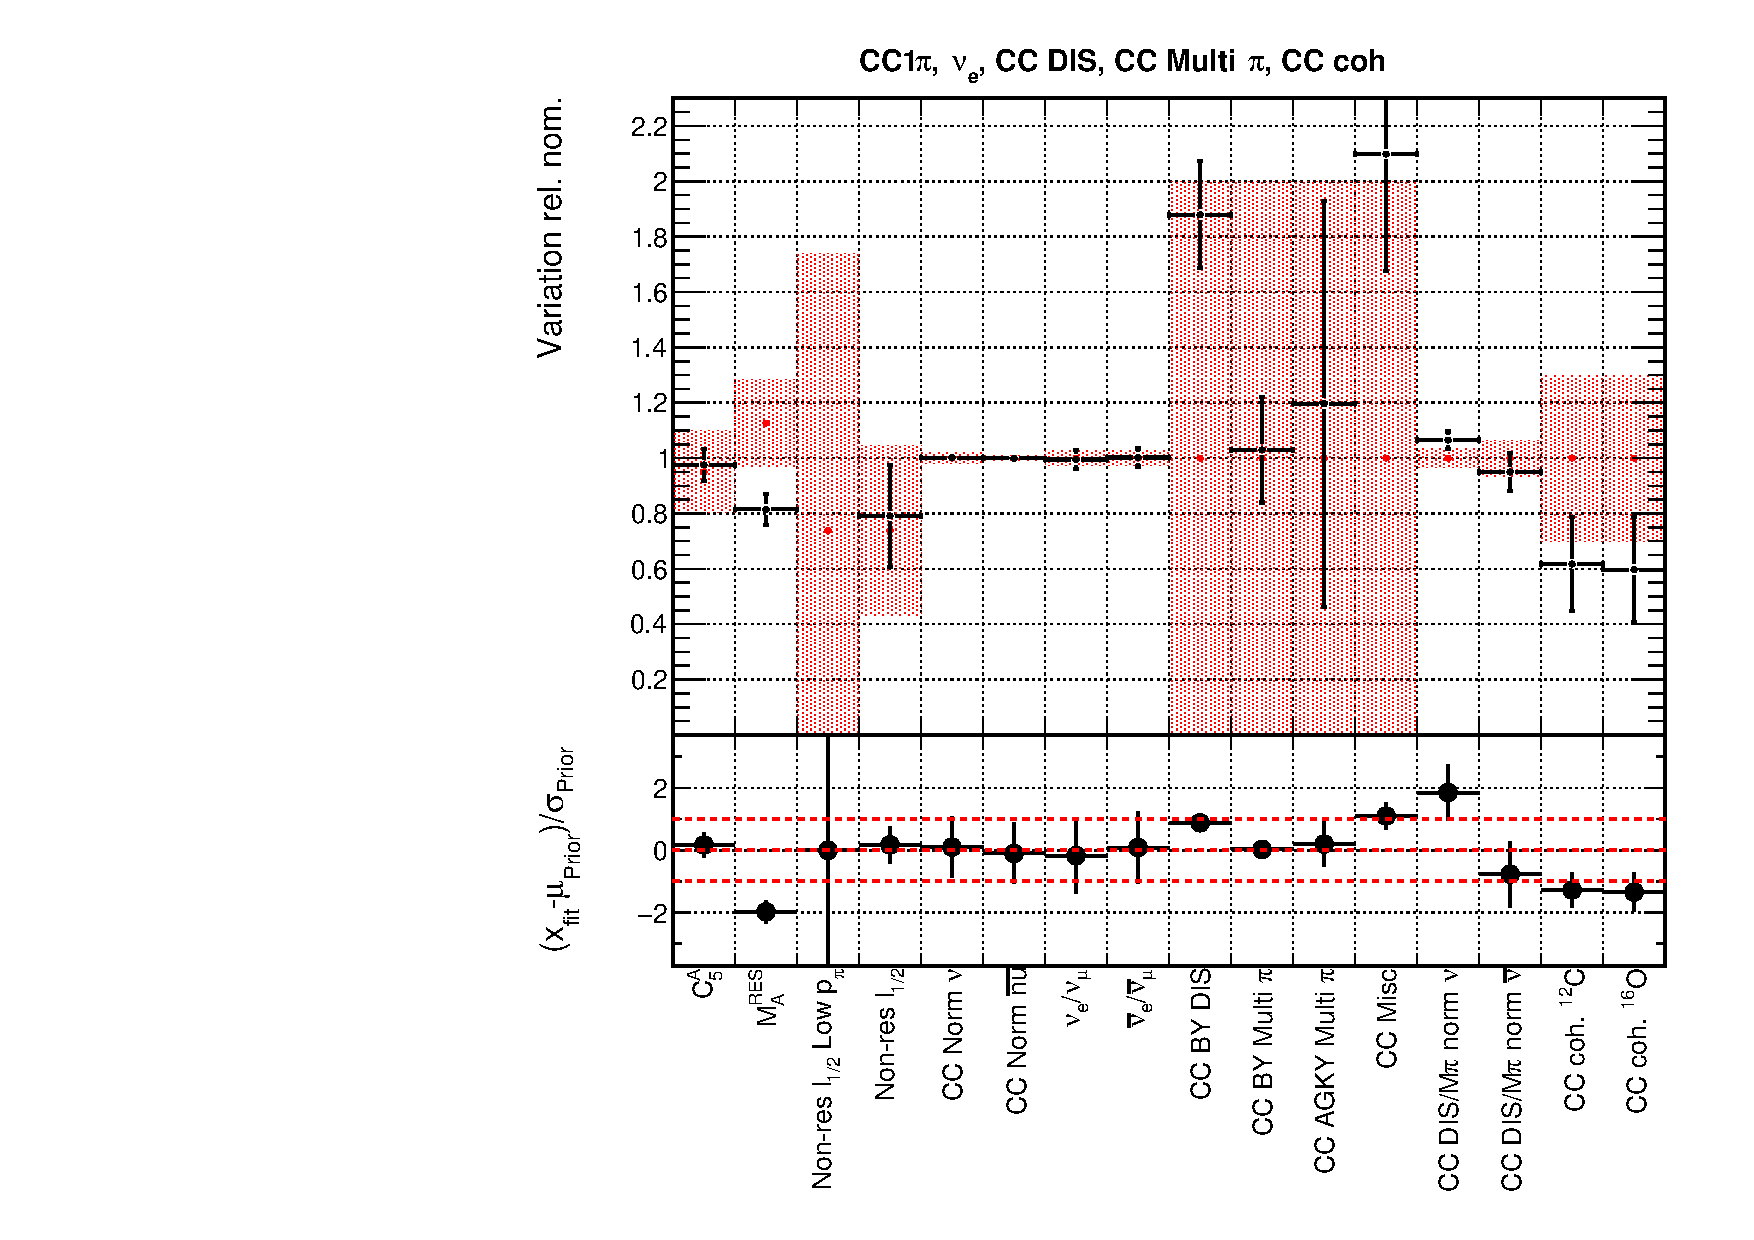
\includegraphics[width=0.9\linewidth]{figs/datxsec3}
  \caption{CC 1$\pi$, $\nu_e$, CC DIS, CC multi-$\pi$ and CC coh.}
\end{subfigure}
\begin{subfigure}{0.45\textwidth}
  \centering
  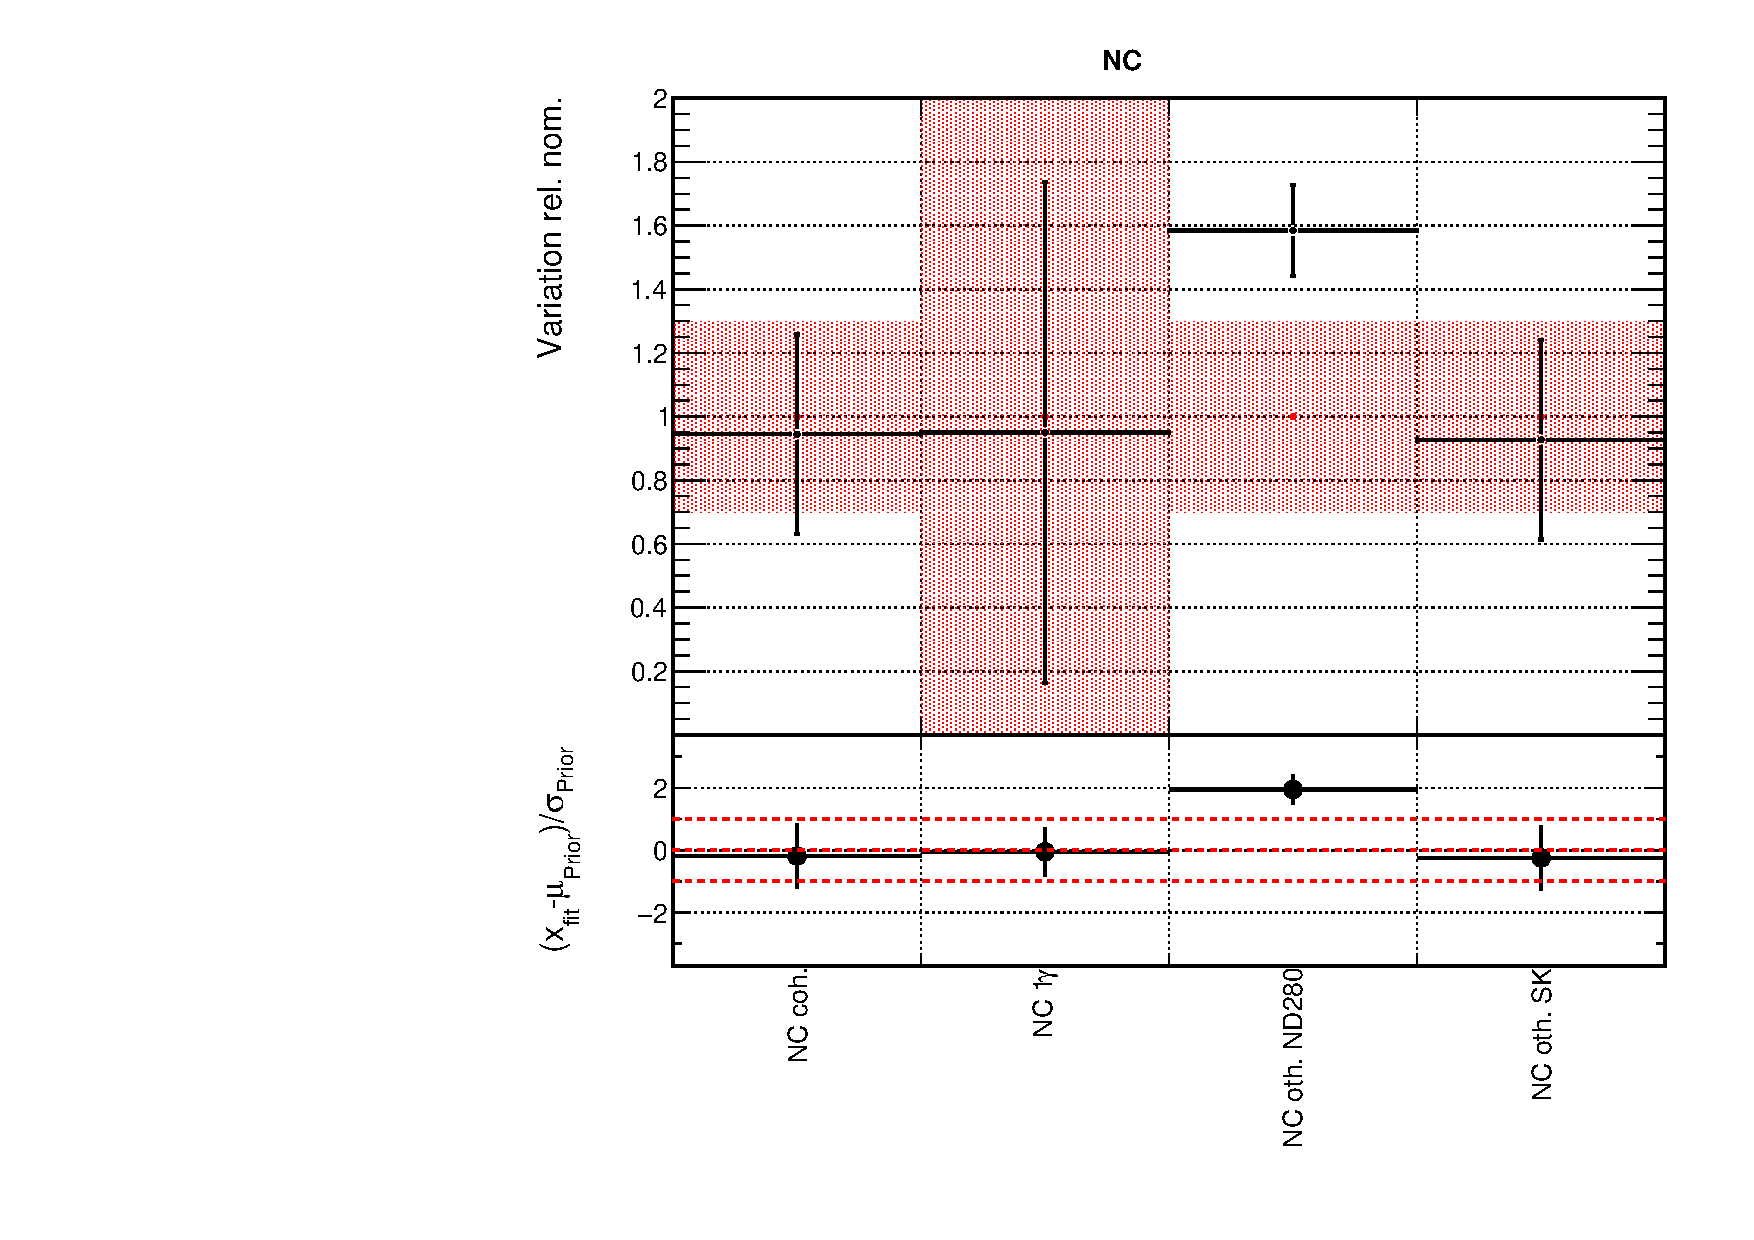
\includegraphics[width=0.9\linewidth]{figs/datxsec4}
  \caption{NC}
\end{subfigure}
\begin{subfigure}{0.49\textwidth}
  \centering
  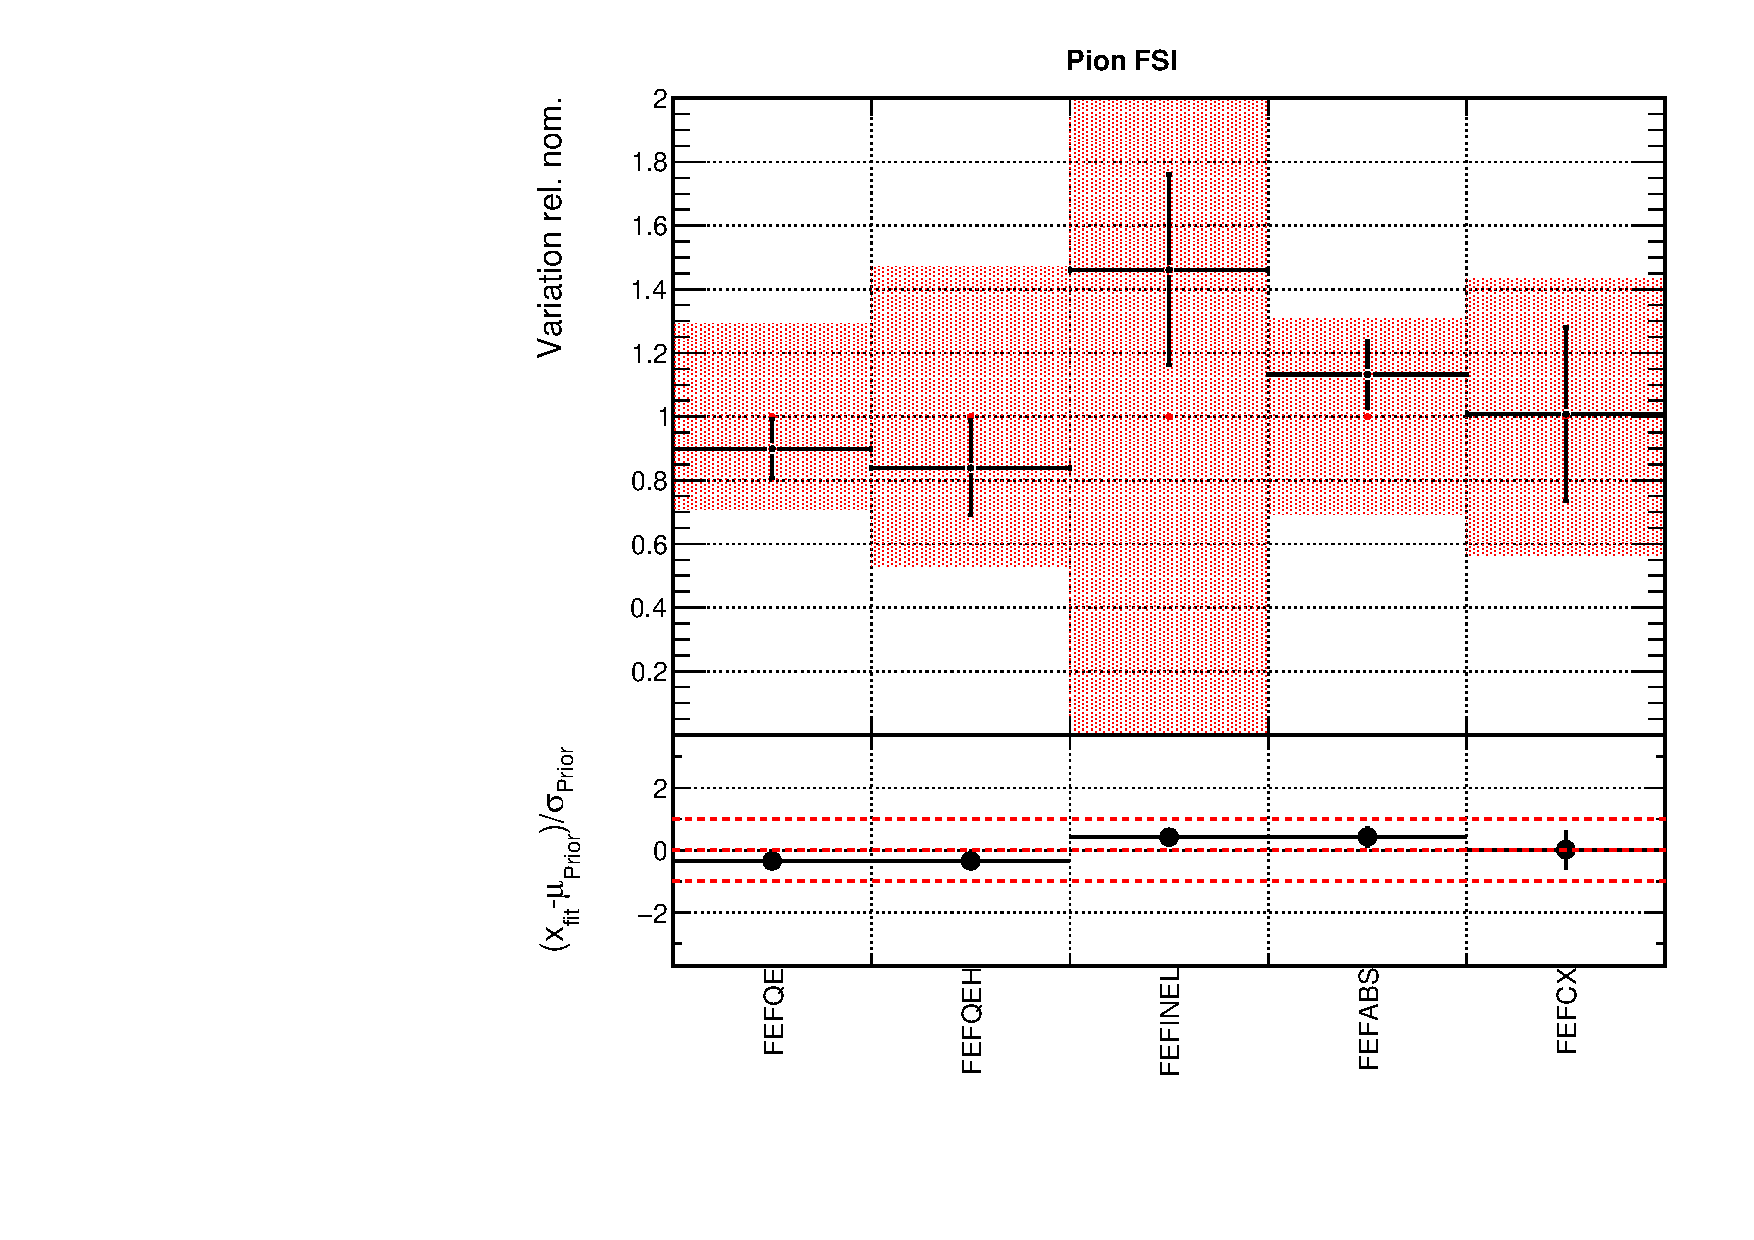
\includegraphics[width=0.9\linewidth]{figs/datxsec5}
  \caption{$\pi$ FSI}
\end{subfigure}
\caption{Interaction parameters for the data fit.}
\label{fig:datxsecapp}
\end{figure}

The results for the Asimov fits comparing different fit and detector binnings are shown in Figures \ref{fig:polyasmvsfluxNDapp}, \ref{fig:polyasmvsfluxSKapp} and \ref{fig:polyasmvsxsecapp}.

\begin{figure}[!htbp]
\centering
\begin{subfigure}{0.3\textwidth}
  \centering
  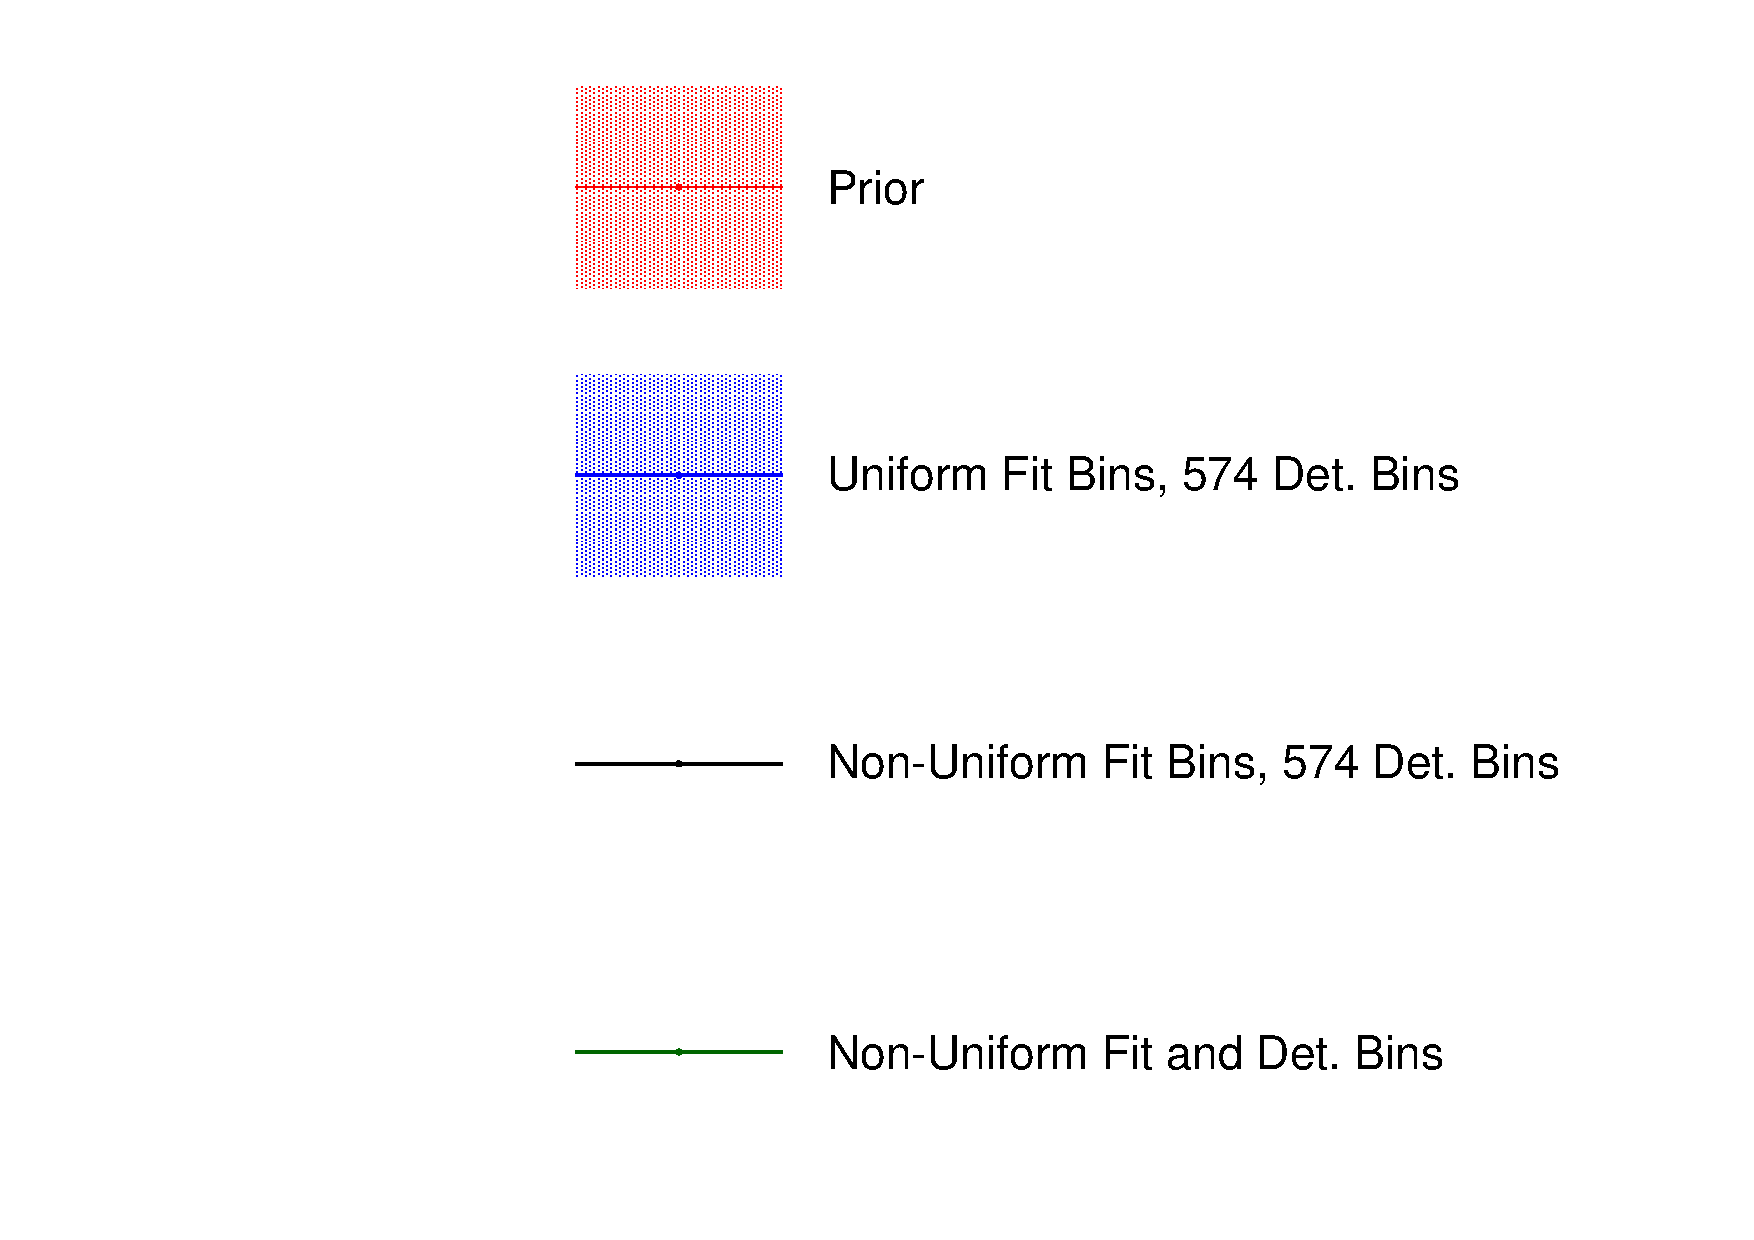
\includegraphics[width=1.0\linewidth,  trim={5mm  80mm 0mm 0mm}, clip]{figs/polyasmvs_leg}
\end{subfigure}
\begin{subfigure}{0.3\textwidth}
  \centering
  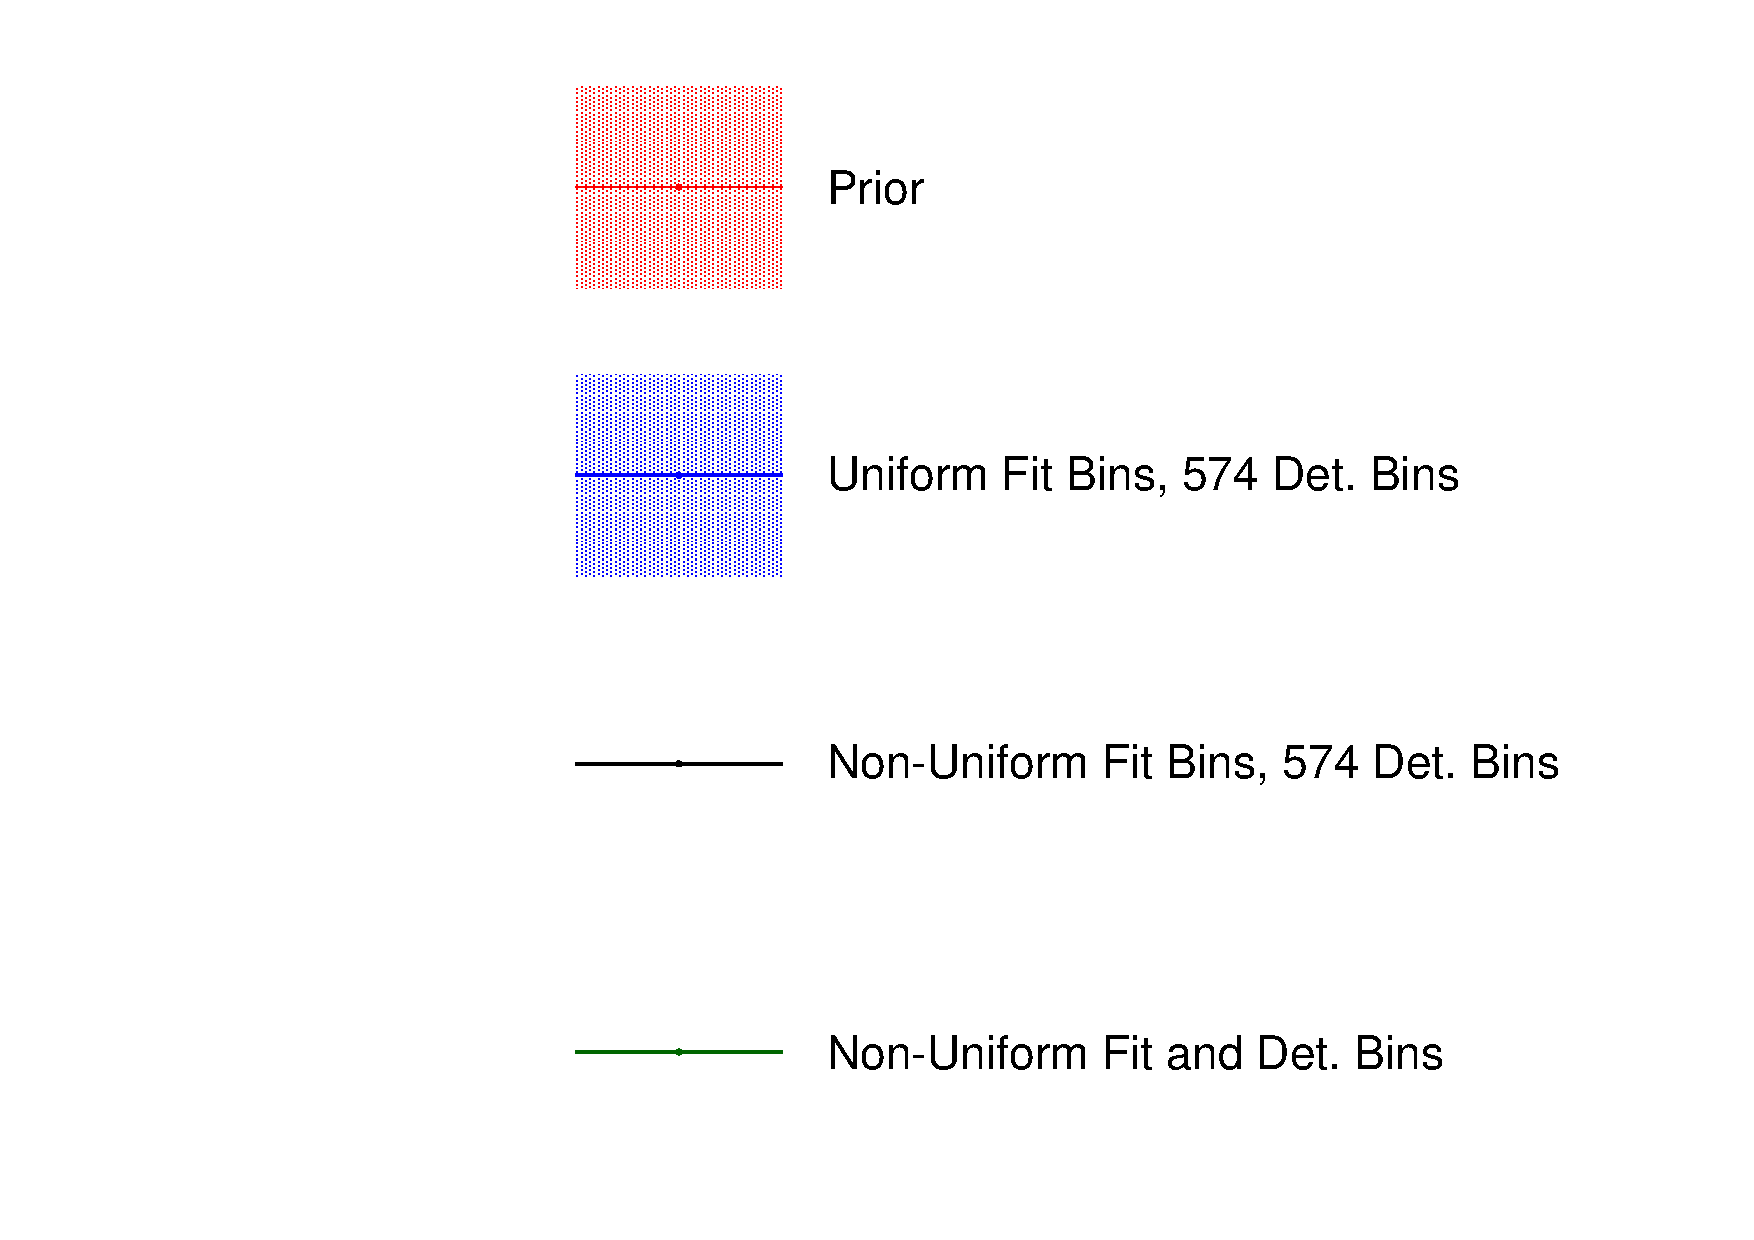
\includegraphics[width=1.0\linewidth,  trim={5mm  0mm 0mm 95mm}, clip]{figs/polyasmvs_leg}
\end{subfigure}
\begin{subfigure}{0.45\textwidth}
  \centering
  \includegraphics[width=0.75\linewidth]{figs/polyasmvsflux_0}
  \caption{ND FHC $\nu_{\mu}$}
\end{subfigure}
\begin{subfigure}{0.45\textwidth}
  \centering
  \includegraphics[width=0.75\linewidth]{figs/polyasmvsflux_1}
  \caption{ND FHC $\bar{\nu_{\mu}}$}
\end{subfigure}
\begin{subfigure}{0.45\textwidth}
  \centering
  \includegraphics[width=0.75\linewidth]{figs/polyasmvsflux_2}
  \caption{ND FHC $\nu_{e}$}
\end{subfigure}
\begin{subfigure}{0.45\textwidth}
  \centering
  \includegraphics[width=0.75\linewidth]{figs/polyasmvsflux_3}
  \caption{ND FHC $\bar{\nu_{e}}$}
\end{subfigure}
\begin{subfigure}{0.45\textwidth}
  \centering
  \includegraphics[width=0.75\linewidth]{figs/polyasmvsflux_4}
  \caption{ND RHC $\nu_{\mu}$}
\end{subfigure}
\begin{subfigure}{0.45\textwidth}
  \centering
  \includegraphics[width=0.75\linewidth]{figs/polyasmvsflux_5}
  \caption{ND RHC $\bar{\nu_{\mu}}$}
\end{subfigure}
\begin{subfigure}{0.45\textwidth}
  \centering
  \includegraphics[width=0.75\linewidth]{figs/polyasmvsflux_6}
  \caption{ND RHC $\nu_{e}$}
\end{subfigure}
\begin{subfigure}{0.45\textwidth}
  \centering
  \includegraphics[width=0.75\linewidth]{figs/polyasmvsflux_7}
  \caption{ND RHC $\bar{\nu_e}$}
\end{subfigure}
\caption{Comparison of ND280 flux parameters for the Asimov fits with different fit and detector binnings.}
\label{fig:polyasmvsfluxNDapp}
\end{figure}

\begin{figure}[!htbp]
\centering
\begin{subfigure}{0.3\textwidth}
  \centering
  \includegraphics[width=1.0\linewidth,  trim={5mm  80mm 0mm 0mm}, clip]{figs/polyasmvs_leg}
\end{subfigure}
\begin{subfigure}{0.3\textwidth}
  \centering
  \includegraphics[width=1.0\linewidth,  trim={5mm  0mm 0mm 95mm}, clip]{figs/polyasmvs_leg}
\end{subfigure}
\begin{subfigure}{0.45\textwidth}
  \centering
  \includegraphics[width=0.75\linewidth]{figs/polyasmvsflux_8}
  \caption{\SK FHC $\nu_{\mu}$}
\end{subfigure}
\begin{subfigure}{0.45\textwidth}
  \centering
  \includegraphics[width=0.75\linewidth]{figs/polyasmvsflux_9}
  \caption{\SK FHC $\bar{\nu_{\mu}}$}
\end{subfigure}
\begin{subfigure}{0.45\textwidth}
  \centering
  \includegraphics[width=0.75\linewidth]{figs/polyasmvsflux_10}
  \caption{\SK FHC $\nu_{e}$}
\end{subfigure}
\begin{subfigure}{0.45\textwidth}
  \centering
  \includegraphics[width=0.75\linewidth]{figs/polyasmvsflux_11}
  \caption{\SK FHC $\bar{\nu_{e}}$}
\end{subfigure}
\begin{subfigure}{0.45\textwidth}
  \centering
  \includegraphics[width=0.75\linewidth]{figs/polyasmvsflux_12}
  \caption{\SK RHC $\nu_{\mu}$}
\end{subfigure}
\begin{subfigure}{0.45\textwidth}
  \centering
  \includegraphics[width=0.75\linewidth]{figs/polyasmvsflux_13}
  \caption{\SK RHC $\bar{\nu_{\mu}}$}
\end{subfigure}
\begin{subfigure}{0.45\textwidth}
  \centering
  \includegraphics[width=0.75\linewidth]{figs/polyasmvsflux_14}
  \caption{\SK RHC $\nu_{e}$}
\end{subfigure}
\begin{subfigure}{0.45\textwidth}
  \centering
  \includegraphics[width=0.75\linewidth]{figs/polyasmvsflux_15}
  \caption{\SK RHC $\bar{\nu_e}$}
\end{subfigure}
\caption{Comparison of \SK flux parameters for the Asimov fits with different fit and detector binnings.}
\label{fig:polyasmvsfluxSKapp}
\end{figure}

\begin{figure}[!htbp]
\centering
\begin{subfigure}{0.3\textwidth}
  \centering
  \includegraphics[width=1.0\linewidth,  trim={5mm  80mm 0mm 0mm}, clip]{figs/polyasmvs_leg}
\end{subfigure}
\begin{subfigure}{0.3\textwidth}
  \centering
  \includegraphics[width=1.0\linewidth,  trim={5mm  0mm 0mm 95mm}, clip]{figs/polyasmvs_leg}
\end{subfigure}
\begin{subfigure}{0.49\textwidth}
  \centering
  \includegraphics[width=0.9\linewidth]{figs/polyasmvsxsec_1}
  \caption{CC 0$\pi$}
\end{subfigure}
\begin{subfigure}{0.49\textwidth}
  \centering
  \includegraphics[width=0.9\linewidth]{figs/polyasmvsxsec_2}
  \caption{$Q^2$ and $E_{\mathrm{b}}$}
\end{subfigure}
\begin{subfigure}{0.49\textwidth}
  \centering
  \includegraphics[width=0.9\linewidth]{figs/polyasmvsxsec_3}
  \caption{CC 1$\pi$, $\nu_e$, CC DIS, CC multi-$\pi$ and CC Coh.}
\end{subfigure}
\begin{subfigure}{0.49\textwidth}
  \centering
  \includegraphics[width=0.9\linewidth]{figs/polyasmvsxsec_4}
  \caption{NC}
\end{subfigure}
\begin{subfigure}{0.49\textwidth}
  \centering
  \includegraphics[width=0.9\linewidth]{figs/polyasmvsxsec_5}
  \caption{$\pi$ FSI}
\end{subfigure}
\caption{Comparison of interaction parameters for the Asimov fits with different fit and detector binnings.}
\label{fig:polyasmvsxsecapp}
\end{figure}

The results for the data fits comparing different fit and detector binnings are shown in Figures \ref{fig:polydatafluxNDapp}, \ref{fig:polydatafluxSKapp} and \ref{fig:polydataxsecapp}.

\begin{figure}[!htbp]
\centering
\begin{subfigure}{0.3\textwidth}
  \centering
  \includegraphics[width=1.0\linewidth,  trim={5mm  80mm 0mm 0mm}, clip]{figs/polyasmvs_leg}
\end{subfigure}
\begin{subfigure}{0.3\textwidth}
  \centering
  \includegraphics[width=1.0\linewidth,  trim={5mm  0mm 0mm 95mm}, clip]{figs/polyasmvs_leg}
\end{subfigure}
\begin{subfigure}{0.45\textwidth}
  \centering
  \includegraphics[width=0.75\linewidth]{figs/polydataflux_0}
  \caption{ND FHC $\nu_{\mu}$}
\end{subfigure}
\begin{subfigure}{0.45\textwidth}
  \centering
  \includegraphics[width=0.75\linewidth]{figs/polydataflux_1}
  \caption{ND FHC $\bar{\nu_{\mu}}$}
\end{subfigure}
\begin{subfigure}{0.45\textwidth}
  \centering
  \includegraphics[width=0.75\linewidth]{figs/polydataflux_2}
  \caption{ND FHC $\nu_e$}
\end{subfigure}
\begin{subfigure}{0.45\textwidth}
  \centering
  \includegraphics[width=0.75\linewidth]{figs/polydataflux_3}
  \caption{ND FHC $\bar{\nu_{e}}$}
\end{subfigure}
\begin{subfigure}{0.45\textwidth}
  \centering
  \includegraphics[width=0.75\linewidth]{figs/polydataflux_4}
  \caption{ND RHC $\nu_{\mu}$}
\end{subfigure}
\begin{subfigure}{0.45\textwidth}
  \centering
  \includegraphics[width=0.75\linewidth]{figs/polydataflux_5}
  \caption{ND RHC $\bar{\nu_{\mu}}$}
\end{subfigure}
\begin{subfigure}{0.45\textwidth}
  \centering
  \includegraphics[width=0.75\linewidth]{figs/polydataflux_6}
  \caption{ND RHC $\nu_{e}$}
\end{subfigure}
\begin{subfigure}{0.45\textwidth}
  \centering
  \includegraphics[width=0.75\linewidth]{figs/polydataflux_7}
  \caption{ND RHC $\bar{\nu_{e}}$}
\end{subfigure}
\caption{Comparison of ND280 flux parameters for the data fits with different fit and detector binnings.}
\label{fig:polydatafluxNDapp}
\end{figure}

\begin{figure}[!htbp]
\centering
\begin{subfigure}{0.3\textwidth}
  \centering
  \includegraphics[width=1.0\linewidth,  trim={5mm  80mm 0mm 0mm}, clip]{figs/polyasmvs_leg}
\end{subfigure}
\begin{subfigure}{0.3\textwidth}
  \centering
  \includegraphics[width=1.0\linewidth,  trim={5mm  0mm 0mm 95mm}, clip]{figs/polyasmvs_leg}
\end{subfigure}
\begin{subfigure}{0.45\textwidth}
  \centering
  \includegraphics[width=0.75\linewidth]{figs/polydataflux_8}
  \caption{\SK FHC $\nu_{\mu}$}
\end{subfigure}
\begin{subfigure}{0.45\textwidth}
  \centering
  \includegraphics[width=0.75\linewidth]{figs/polydataflux_9}
  \caption{\SK FHC $\bar{\nu_{\mu}}$}
\end{subfigure}
\begin{subfigure}{0.45\textwidth}
  \centering
  \includegraphics[width=0.75\linewidth]{figs/polydataflux_10}
  \caption{\SK FHC $\nu_e$}
\end{subfigure}
\begin{subfigure}{0.45\textwidth}
  \centering
  \includegraphics[width=0.75\linewidth]{figs/polydataflux_11}
  \caption{\SK FHC $\bar{\nu_{e}}$}
\end{subfigure}
\begin{subfigure}{0.45\textwidth}
  \centering
  \includegraphics[width=0.75\linewidth]{figs/polydataflux_12}
  \caption{\SK RHC $\nu_{\mu}$}
\end{subfigure}
\begin{subfigure}{0.45\textwidth}
  \centering
  \includegraphics[width=0.75\linewidth]{figs/polydataflux_13}
  \caption{\SK RHC $\bar{\nu_{\mu}}$}
\end{subfigure}
\begin{subfigure}{0.45\textwidth}
  \centering
  \includegraphics[width=0.75\linewidth]{figs/polydataflux_14}
  \caption{\SK RHC $\nu_{e}$}
\end{subfigure}
\begin{subfigure}{0.45\textwidth}
  \centering
  \includegraphics[width=0.75\linewidth]{figs/polydataflux_15}
  \caption{\SK RHC $\bar{\nu_e}$}
\end{subfigure}
\caption{Comparison of \SK flux parameters for the data fits with different fit and detector binnings.}
\label{fig:polydatafluxSKapp}
\end{figure}

\begin{figure}[!htbp]
\centering
\begin{subfigure}{0.3\textwidth}
  \centering
  \includegraphics[width=1.0\linewidth,  trim={5mm  80mm 0mm 0mm}, clip]{figs/polyasmvs_leg}
\end{subfigure}
\begin{subfigure}{0.3\textwidth}
  \centering
  \includegraphics[width=1.0\linewidth,  trim={5mm  0mm 0mm 95mm}, clip]{figs/polyasmvs_leg}
\end{subfigure}
\begin{subfigure}{0.49\textwidth}
  \centering
  \includegraphics[width=0.9\linewidth]{figs/polydataxsec_1}
  \caption{CC 0$\pi$}
\end{subfigure}
\begin{subfigure}{0.49\textwidth}
  \centering
  \includegraphics[width=0.9\linewidth]{figs/polydataxsec_2}
  \caption{$Q^2$ and $E_{\mathrm{b}}$}
\end{subfigure}
\begin{subfigure}{0.49\textwidth}
  \centering
  \includegraphics[width=0.9\linewidth]{figs/polydataxsec_3}
  \caption{CC 1$\pi$, $\nu_e$, CC DIS, CC multi-$\pi$ and CC Coh.}
\end{subfigure}
\begin{subfigure}{0.49\textwidth}
  \centering
  \includegraphics[width=0.9\linewidth]{figs/polydataxsec_4}
  \caption{NC}
\end{subfigure}
\begin{subfigure}{0.49\textwidth}
  \centering
  \includegraphics[width=0.9\linewidth]{figs/polydataxsec_5}
  \caption{$\pi$ FSI}
\end{subfigure}
\caption{Comparison of interaction parameters for the data fits with different fit and detector binnings.}
\label{fig:polydataxsecapp}
\end{figure}

The joint near and far, and near detector only fits are compared in Figures \ref{fig:jointfluxNDapp}, \ref{fig:jointfluxSKapp} and \ref{fig:jointxsecapp}.

\begin{figure}[!htbp]
\centering
\begin{subfigure}{0.8\textwidth}
  \centering
  \includegraphics[width=0.24\linewidth]{figs/joint_leg}
\end{subfigure}
\begin{subfigure}{0.45\textwidth}
  \centering
  \includegraphics[width=0.75\linewidth]{figs/jointflux0}
  \caption{ND FHC $\nu_{\mu}$}
\end{subfigure}
\begin{subfigure}{0.45\textwidth}
  \centering
  \includegraphics[width=0.75\linewidth]{figs/jointflux1}
  \caption{ND FHC $\bar{\nu_{\mu}}$}
\end{subfigure}
\begin{subfigure}{0.45\textwidth}
  \centering
  \includegraphics[width=0.75\linewidth]{figs/jointflux2}
  \caption{ND FHC $\nu_{e}$}
\end{subfigure}
\begin{subfigure}{0.45\textwidth}
  \centering
  \includegraphics[width=0.75\linewidth]{figs/jointflux3}
  \caption{ND FHC $\bar{\nu_{e}}$}
\end{subfigure}
\begin{subfigure}{0.45\textwidth}
  \centering
  \includegraphics[width=0.75\linewidth]{figs/jointflux4}
  \caption{ND RHC $\nu_{\mu}$}
\end{subfigure}
\begin{subfigure}{0.45\textwidth}
  \centering
  \includegraphics[width=0.75\linewidth]{figs/jointflux5}
  \caption{ND RHC $\bar{\nu_{\mu}}$}
\end{subfigure}
\begin{subfigure}{0.45\textwidth}
  \centering
  \includegraphics[width=0.75\linewidth]{figs/jointflux6}
  \caption{ND RHC $\nu_{e}$}
\end{subfigure}
\begin{subfigure}{0.45\textwidth}
  \centering
  \includegraphics[width=0.75\linewidth]{figs/jointflux7}
  \caption{ND RHC $\bar{\nu_e}$}
\end{subfigure}
\caption{ND280 flux parameters for the joint and near detector only fits.}
\label{fig:jointfluxNDapp}
\end{figure}

\begin{figure}[!htbp]
\centering
\begin{subfigure}{0.8\textwidth}
  \centering
  \includegraphics[width=0.24\linewidth]{figs/joint_leg}
\end{subfigure}
\begin{subfigure}{0.45\textwidth}
  \centering
  \includegraphics[width=0.75\linewidth]{figs/jointflux8}
  \caption{\SK FHC $\nu_{\mu}$}
\end{subfigure}
\begin{subfigure}{0.45\textwidth}
  \centering
  \includegraphics[width=0.75\linewidth]{figs/jointflux9}
  \caption{\SK FHC $\bar{\nu_{\mu}}$}
\end{subfigure}
\begin{subfigure}{0.45\textwidth}
  \centering
  \includegraphics[width=0.75\linewidth]{figs/jointflux10}
  \caption{\SK FHC $\nu_{e}$}
\end{subfigure}
\begin{subfigure}{0.45\textwidth}
  \centering
  \includegraphics[width=0.75\linewidth]{figs/jointflux11}
  \caption{\SK FHC $\bar{\nu_{e}}$}
\end{subfigure}
\begin{subfigure}{0.45\textwidth}
  \centering
  \includegraphics[width=0.75\linewidth]{figs/jointflux12}
  \caption{\SK RHC $\nu_{\mu}$}
\end{subfigure}
\begin{subfigure}{0.45\textwidth}
  \centering
  \includegraphics[width=0.75\linewidth]{figs/jointflux13}
  \caption{\SK RHC $\bar{\nu_{\mu}}$}
\end{subfigure}
\begin{subfigure}{0.45\textwidth}
  \centering
  \includegraphics[width=0.75\linewidth]{figs/jointflux14}
  \caption{\SK RHC $\nu_{e}$}
\end{subfigure}
\begin{subfigure}{0.45\textwidth}
  \centering
  \includegraphics[width=0.75\linewidth]{figs/jointflux15}
  \caption{\SK RHC $\bar{\nu_e}$}
\end{subfigure}
\caption{\SK flux parameters for the joint and near detector only fits.}
\label{fig:jointfluxSK}
\end{figure}

\begin{figure}[!htbp]
\centering
\begin{subfigure}{0.8\textwidth}
  \centering
  \includegraphics[width=0.24\linewidth]{figs/joint_leg}
\end{subfigure}
\begin{subfigure}{0.49\textwidth}
  \centering
  \includegraphics[width=0.9\linewidth]{figs/jointxsec1}
  \caption{CC 0$\pi$}
\end{subfigure}
\begin{subfigure}{0.49\textwidth}
  \centering
  \includegraphics[width=0.9\linewidth]{figs/jointxsec2}
  \caption{$Q^2$ and $E_{\mathrm{b}}$}
\end{subfigure}
\begin{subfigure}{0.49\textwidth}
  \centering
  \includegraphics[width=0.9\linewidth]{figs/jointxsec3}
  \caption{CC 1$\pi$, $\nu_e$, CC DIS, CC multi-$\pi$ and CC coh.}
\end{subfigure}
\begin{subfigure}{0.45\textwidth}
  \centering
  \includegraphics[width=0.9\linewidth]{figs/jointxsec4}
  \caption{NC}
\end{subfigure}
\begin{subfigure}{0.49\textwidth}
  \centering
  \includegraphics[width=0.9\linewidth]{figs/jointxsec5}
  \caption{$\pi$ FSI}
\end{subfigure}
\caption{Interaction parameters for the joint and near detector only fits.}
\label{fig:jointxsecapp}
\end{figure}

\newpage 
